\chapterimage{chap1.jpg}
\chapter{预备知识}
\begin{introduction}
	\item 函数定义和性质
	\item 基本不等式
	\item 柯西不等式
	\item 三角函数和反三角函数
	\item 特殊函数
\end{introduction}
\section{函数}
\begin{definition}[函数]
	1. 函数定义:
	
	$X,Y$ 是给定的两个集合, 若对于任意 $x\in X$, 存在法则 $f$, 使得唯一的 $y = f(x)$ 满足 $y\in Y$, 则称 $f$ 为从 $X$ 到 $Y$ 的一个函数, 记为 $f:X\to Y$, 其中 $X$ 称为定义域, $f(x)(x\in X)$ 称为值域
	
	2. 函数的三要素: 定义域、对应法则和值域
\end{definition}

\begin{definition}[函数的基本性质]
	\begin{enumerate}
		\item 单射: 若对于任意 $x_{1},x_{2}\in X$, 若 $x_{1}\neq x_{2}$, 则 $f(x_{1})\neq f(x_{2})$
		\item 满射: 若对于任意 $y\in Y$, 存在 $x\in X$, 使得 $f(x)=y$
		\item 双射: 若 $f$ 既是单射又是满射
	\end{enumerate}
\end{definition}

\begin{definition}[函数基本运算]
	\begin{enumerate}
		\item 基本四则运算
		\item 复合运算
		\item 反函数运算
	\end{enumerate}
\end{definition}

\begin{property}[函数四大性质]
	\begin{itemize}
		\item 有界性
		\item 奇偶性: $\begin{cases} \text{奇函数: }f(-x) = -f(-x) \\ \text{偶函数: }f(-x) = f(x) \end{cases}$
		\item 周期性: $f(x+T) = f(x)$
		\item 单调性: $\forall x_{1},x_{2}\in I (x_{1}\neq x_{2}),\dfrac{f(x_{1})-f(x_{2})}{x_{1}-x_{2}}>(<)0$, $f(x)$ 单调递增(减)
	\end{itemize}
\end{property}

\begin{corollary}[奇偶性推论]
	任意一个定义在 $[-l,l]$ 上的函数 $f(x)$ 均可以写成一个奇函数和一个偶函数的和 $f(x)=h(x)+g(x)$, 其中 $h(x)=\dfrac{f(x)+f(-x)}{2}$ 是偶函数, $g(x)=\dfrac{f(x)-f(-x)}{2}$ 是奇函数
\end{corollary}

\begin{corollary}[周期性、中心对称性、轴对称性]
	
	(1). $f(x)$有对称中心$(a,c)$,且关于直线$x=b$轴对称,我们可以推出$f(x)$的一个周期$T=4|b-a|$.
	
	(2). $f(x)$有两个对称中心$(a,c)$和$(b,c)$,我们可以推出$f(x)$的一个周期$T=2|b-a|$.
	
	(3). $f(x)$有两个对称轴直线$x=a$和直线$x=b$,我们可以推出$f(x)$的一个周期$T=2|b-a|$.

\end{corollary}
\begin{anymark}[证明]
	(1).
	$$\begin{cases} f(2a-x)+f(x)=2c  \\ f(2b-x) = f(x)\end{cases}\to \begin{cases} f(2a-x) + f(2b-x) =2c\\ f(2a-2b+x) +f(x) =2c  \end{cases}\to f(x) = f(x+4a-4b)$$

	(2).
	$$\begin{cases} f(2a-x) = f(2b-x)  \\ f(2a-2b+x) = f(x) \end{cases}\to f(x) = f(x+2a-2b)$$

	(3).
	$$\begin{cases} f(2a-x) = f(x)  \\ f(2b-x) = f(x)\end{cases}\to \begin{cases} f(2a-x) = f(2b-x) \\ f(2a-2b+x) = f(x)   \end{cases}\to f(x) = f(x+2a-2b)$$
\end{anymark}

\subsection{初等函数}
\begin{definition}[初等函数]
	初等函数是指可以用有限次基本初等函数和有限次代数运算得到的函数, 六种基本初等函数:
	\begin{enumerate}
		\item 常数函数: $y=C$
		\item 幂函数: $y=x^{\alpha},\alpha\in \mathbb{R}^{*}$
		\item 指数函数: $y=a^{x},a>0,a\neq 1$
		\item 对数函数: $y=\log_{a}x,a>0,a\neq 1$
		\item 三角函数: $y=\sin x, y=\cos x, y=\tan x, y=\cot x, y=\sec x, y=\csc x$
		\item 反三角函数: $y=\arcsin x, y=\arccos x, y=\arctan x, y=\cot^{-1}(x), y=\sec^{-1}(x), y=\csc^{-1}(x)$
	\end{enumerate}
\end{definition}

\subsection{三角函数和反三角函数}
\begin{theorem}[积化和差\& 和差化积\& 倍角公式]
	积化和差公式:
	$$\sin\alpha\sin\beta=\dfrac{1}{2}[\cos(\alpha-\beta)-\cos(\alpha+\beta)]$$
	$$\cos\alpha\cos\beta=\dfrac{1}{2}[\cos(\alpha-\beta)+\cos(\alpha+\beta)]$$
	$$\sin\alpha\cos\beta=\dfrac{1}{2}[\sin(\alpha+\beta)+\sin(\alpha-\beta)]$$
	$$\cos\alpha\sin\beta=\dfrac{1}{2}[\sin(\alpha+\beta)-\sin(\alpha-\beta)]$$
	和差化积公式:
	$$\sin\alpha+\sin\beta=2\sin\dfrac{\alpha+\beta}{2}\cos\dfrac{\alpha-\beta}{2}$$
	$$\sin\alpha-\sin\beta=2\cos\dfrac{\alpha+\beta}{2}\sin\dfrac{\alpha-\beta}{2}$$
	$$\cos\alpha+\cos\beta=2\cos\dfrac{\alpha+\beta}{2}\cos\dfrac{\alpha-\beta}{2}$$
	$$\cos\alpha-\cos\beta=-2\sin\dfrac{\alpha+\beta}{2}\sin\dfrac{\alpha-\beta}{2}$$
	倍角公式:
	$$\sin 2\alpha = 2\sin\alpha\cos\alpha$$
	$$\cos 2\alpha = \cos^{2}\alpha-\sin^{2}\alpha = 2\cos^{2}\alpha-1 = 1-2\sin^{2}\alpha$$
	$$\tan 2\alpha = \dfrac{2\tan\alpha}{1-\tan^{2}\alpha}$$
	$$\sin 2\alpha = \dfrac{2\tan \alpha}{1+\tan^{2}\alpha}\qquad \qquad \cos 2\alpha = \dfrac{1-\tan^{2}\alpha}{1+\tan^{2}\alpha}$$
	$$\sin 3\alpha = 3\sin \alpha -4\sin^{3}\alpha\qquad\qquad \cos 3\alpha = 4\cos^{3}\alpha -3\cos \alpha$$
\end{theorem}
\begin{definition}[反三角函数]
	\begin{enumerate}
		\item $\arcsin x$ 的定义域为 $[-1,1]$, 值域为 $[-\dfrac{\pi}{2},\dfrac{\pi}{2}]$
		\item $\arccos x$ 的定义域为 $[-1,1]$, 值域为 $[0,\pi]$
		\item $\arctan x$ 的定义域为 $(-\infty,+\infty)$, 值域为 $(-\dfrac{\pi}{2},\dfrac{\pi}{2})$
	\end{enumerate}
\end{definition}
\begin{figure}[H]
	\centering  %图片全局居中
	\subfigure[$\arcsin(x)\ \&\ \sin (x)$]{
	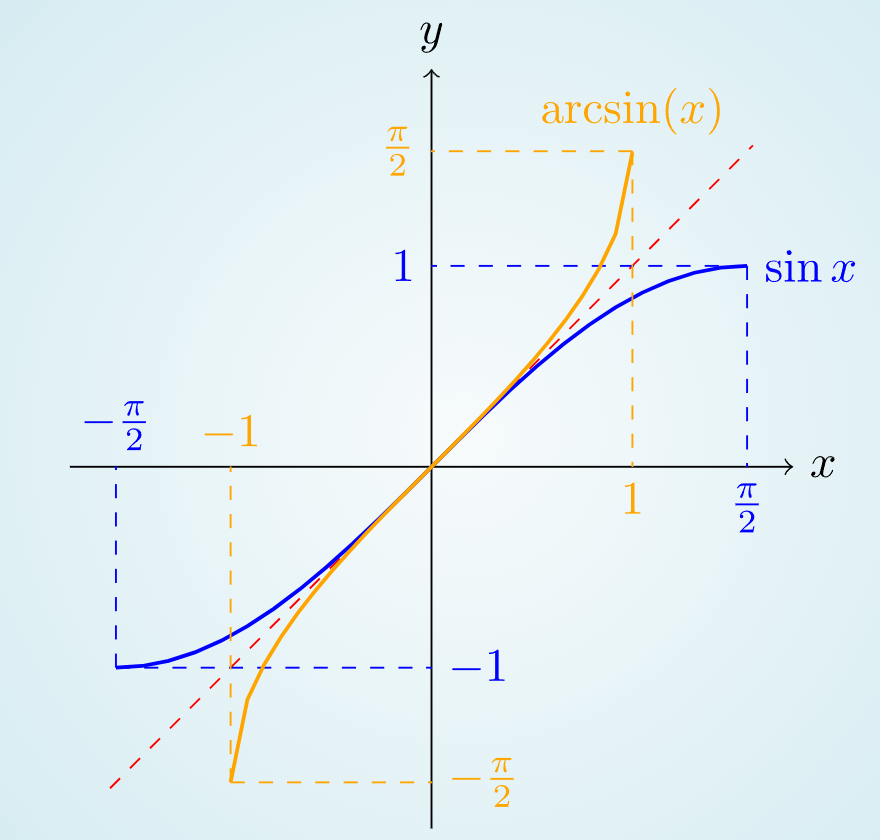
\includegraphics[width=0.4\textwidth]{"figure/Note/arcsinx.png"}}
	\subfigure[$\arccos(x)\ \&\ \cos (x)$]{
	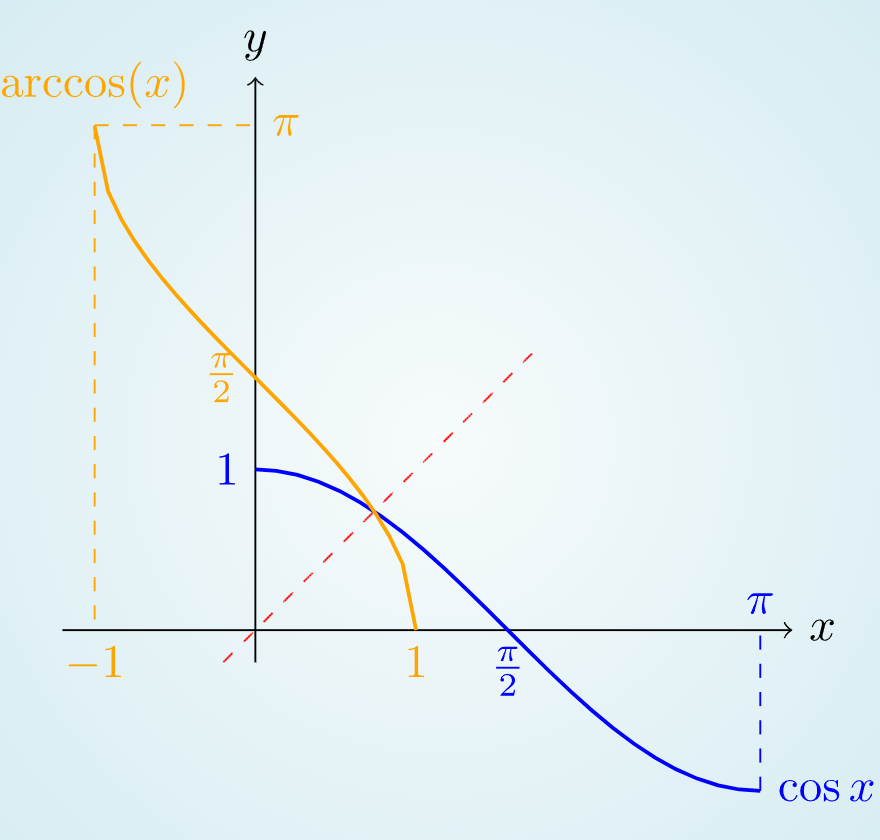
\includegraphics[width=0.4\textwidth]{"figure/Note/arccosx.png"}}
	\subfigure[$\arctan(x)\ \&\ \tan (x)$]{
	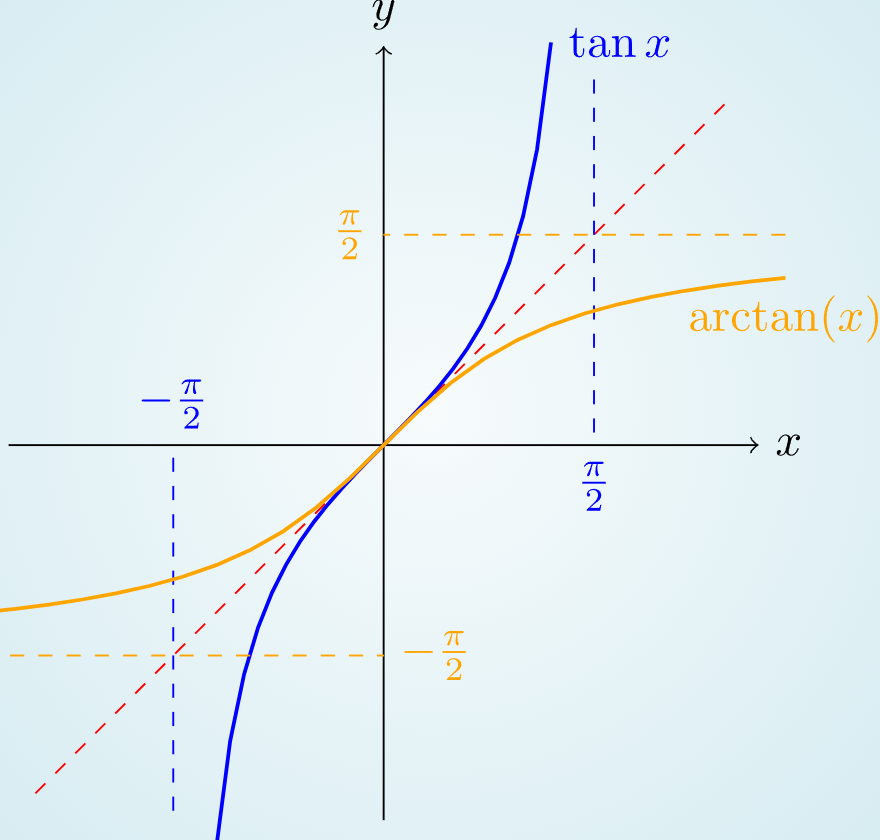
\includegraphics[width=0.4\textwidth]{"figure/Note/arctanx.png"}}
	\caption{反三角函数图像}
\end{figure}
\subsection{特殊函数}
\begin{definition}[特殊函数]
	\begin{enumerate}
		\item 阶乘函数: $$n!=n(n-1)(n-2)\cdots 2\cdot 1, (2n)!! = 2^{n}\cdot n!, 0! = 1$$
		\item 二项式系数: $$\binom{n}{k}=\dfrac{n!}{k!(n-k)!}, (a+b)^{n} = \sum\limits_{i = 0}^{n}\binom{n}{i}a^{i}b^{n-i}$$
		\item 绝对值函数: $$|x|=\begin{cases} x & x\geq 0 \\ -x & x<0 \end{cases}$$
		\item 符号函数: $$sgn(x)=\begin{cases} 1 & x>0 \\ 0 & x=0 \\ -1 & x<0 \end{cases}$$%
		\item 取整函数: $$f(x) = [x], x-1< [x] \leq x, \lim\limits_{x\to 0^{+}} = 0, \lim\limits_{x\to 0^{-}} =-1$$
		\item 分段函数: $$f(x)=\begin{cases} f_{1}(x) & x\in D_{1} \\ f_{2}(x) & x\in D_{2} \\ \cdots \end{cases}$$
		\item 黎曼函数:$$f(x)=\begin{cases} \dfrac{1}{q} & p,q\in \mathbb{Q}, x = \dfrac{p}{q}\in(0,1) \\ 0 & x\notin \mathbb{Q}, x=0,1 \end{cases}$$
		\item 狄利克雷函数: $$f(x)=\begin{cases} 1 & x\in \mathbb{Q} \\ 0 & x\notin \mathbb{Q} \end{cases}$$
	\end{enumerate}
\end{definition}


\begin{theorem}[平均值不等式 $a_{i} > 0$]
	平方平均值:
	$$Q_{n}=\sqrt{\dfrac{\sum\limits_{k=1}^{n}a_{k}^{2}}{n}}$$
	算术平均值:
	$$A_{n}=\dfrac{\sum\limits_{i=1}^{n}a_{i}}{n}$$
	几何平均值:
	$$G_{n}=\sqrt[n]{\prod\limits_{i=1}^{n}a_{i}}$$
	调和平均值:
	$$H_{n}=\dfrac{n}{\sum\limits_{i=1}^{k}\dfrac{1}{a_{i}}}$$
	平均值不等式:
	$$Q_{n}\geq A_{n}\geq G_{n}\geq H_{n}, \text{当且仅当} a_{1} = a_{2} = \cdots = a_{n} \text{等号成立}$$
\end{theorem}

\begin{theorem}[柯西不等式]
	二维形式:
	
	$$(a^{2}+b^{2})(c^{2}+d^{2})\geq (ac+bd)^{2}, \text{当且仅当} ad =bc \text{时等号成立}$$
	
	$n$ 维形式:
	
	$$\left(\sum_{i=1}^{n}a_{i}b_{i}\right)^{2}\leq \left(\sum_{i=1}^{n}a_{i}^{2}\right)\left(\sum_{i=1}^{n}b_{i}^{2}\right),\text{当且仅当} \dfrac{a_{i}}{b_{i}}=c\text{时等号成立}$$
	
	向量形式:

	$$(\alpha,\beta)^{2}\leq (\alpha,\alpha)(\beta,\beta)$$
\end{theorem}
\begin{theorem}[重要不等式]
	\begin{enumerate}
		\item $\sin x < x < \tan x, x\in (0,\dfrac{\pi}{2})\qquad \qquad \arctan x < x < \arcsin x, x\in[0,1]$
		\item $\dfrac{2}{\pi}x < \sin x < x, x\in(0,\dfrac{\pi}{2})\qquad \qquad x < \tan x < \dfrac{4}{\pi}x , x\in(0,\dfrac{\pi}{4})$
		\item $e^{x} \geq x + 1,x\in\mathbb{R}\qquad \qquad x-1 \geq \ln x, x\in(0,+\infty)$
		\item $\dfrac{1}{1+x} < \ln (1+\dfrac{1}{x}) < \dfrac{1}{x}, x\in(0,+\infty)$
	\end{enumerate}
\end{theorem}

\begin{theorem}[重要公式]
	\begin{enumerate}
		\item $\dfrac{n}{(n+1)!} = \dfrac{1}{n!} - \dfrac{1}{(n+1)!}$
		\item $(a^{3}-b^{3}) = (a-b)(a^{2}+ab+b^{2})\qquad\qquad (a^{3}+b^{3}) = (a+b)(a^{2}-ab+b^{2})$
		\item $a^{n} - b^{n} = (a-b)(a^{n-1}-a^{n-2}b+\cdots -ab^{n-2}+b^{n-1})$
		\item $a^{n} + b^{n} = (a+b)(a^{n-1}-a^{n-1}b+\cdots -ab^{n-2} +b^{n-1}), n\in \{2k+1 | k\in \mathbb{N}\}$
	\end{enumerate}
\end{theorem}

\section{函数的表示方法}
\subsection{显式表达}
\begin{definition}[显示表达]
	$y = f(x)$ 初等函数都是显性表达
\end{definition}
\subsection{隐式表达}
\begin{definition}[隐式表达]
	$f(x,y) = 0$ 一般不能用 $x$ 表示 $y$, 也不能用 $y$ 表示 $x$
\end{definition}
\subsection{极坐标}
\begin{definition}[极坐标]
	极坐标系是平面直角坐标系的一种推广, 它是由一个原点 $O$ 和一个射线 $Ox$ 组成的, 其中 $O$ 称为极点, $Ox$ 称为极轴, 
	任意一点 $P$ 到极点 $O$ 的距离 $r$ 叫做点 $P$ 的极径, 点 $P$ 到极轴的角 $\theta$ 叫做点 $P$ 的极角, 记为 $P(r,\theta)$
\end{definition}

\begin{definition}[重要极坐标方程]
	\begin{enumerate}
		\item 圆方程: $r = a, r = a\sin\theta, r = a\cos\theta$
		\item 心形线方程: $r = a(1\pm \cos\theta), r = a(1\pm \sin\theta)$
		\item 阿基米德螺线方程: $r = a\theta$
		\item 三叶玫瑰线方程: $r = a\sin 3\theta, r = a\cos 3\theta$
		\item 伯努利双扭线方程: $r^{2} = a^{2}\cos 2\theta, r^{2} = a^{2}\sin 2\theta$
	\end{enumerate}
\end{definition}
\subsection{参数方程}
\begin{definition}[参数方程]
	$$\begin{cases}
		x = f(t)\\
		y = g(t)
	\end{cases} \qquad t\in[\alpha,\beta]$$
\end{definition}
\begin{definition}[重要参数方程]
	\begin{enumerate}
		\item 摆线方程: $x = a(t-\sin t), y = a(1-\cos t)$
		\item 星形线方程: $x = a\cos^{3} t, y = a\sin^{3} t$
	\end{enumerate}
\end{definition}

\begin{anymark}[注]
	\begin{itemize}
		\item 双曲函数和反双曲函数的定义和性质 $\mathbf{def:}$ \ref{def: 双曲函数}
		\item 常见曲线极坐标和参数方程 $\mathbf{def:}$ \ref{def: 常用曲线}
	\end{itemize} 
\end{anymark}




\chapterimage{chap2.jpg}

\chapter{数列极限}
\begin{introduction}
	\item 数列极限定义和性质
	\item 归结原理
	\item 夹逼准则
	\item 单调有界准则
\end{introduction}
\section{数列极限}
\begin{definition}[数列极限]
	设 $x_{n}$ 是 一数列, 若存在常数 $a$, $\forall \epsilon>0$, $\exists N_{0}>0$, 当 $n>N_{0}$ 时, $|x_{n}-a|<\epsilon$ 恒成立, 常数 $a$ 是数列 $\{x_{n}\}$ 的极限或者说数列 $\{x_{n}\}$ 趋近于 $a$
\end{definition}


\begin{corollary}[唯一性]
	若极限存在, 则极限唯一
\end{corollary}

\begin{corollary}[有界性]
	若数列 $\{x_{n}\}$ 的极限 $a$ 存在, 则数列 $\{x_{n}\}$ 有界
\end{corollary}

\begin{corollary}[保号性]
	若数列 $\{x_{n}\}$ 的极限 $a>0(a<0)$, 则存在正整数 $N_{0}$, 当 $n>N_{0}$ 时, $x_{n}>0(x_{n}<0)$, 取 $\epsilon = \pm a$ 即可
\end{corollary}
\begin{anymark}[注]
	\begin{itemize}
		\item 若数列的任意子列发散, 数列极限不存在
		\item 若数列的任意两个子列极限存在但不相等, 数列极限不存在
	\end{itemize}
\end{anymark}
\begin{corollary}[数列极限]
	\begin{itemize}
		\item 如果数列从某项起有 $x_{n}\geq 0$ 且 $\lim\limits_{n\to\infty}x_{n} = a$, 则 $a\geq 0$
		\item 如果 $\lim\limits_{n\to\infty} x_{n} = A$, 则 $\lim\limits_{n\to\infty} |x_{n}| = |A|$
		\item $\lim\limits_{n\to +\infty}x_{n}=a\to \begin{cases} \lim\limits_{n\to +\infty}\dfrac{x_{n+1}}{x_{n}}=1, & a\neq 0\\ \lim\limits_{n\to +\infty}\dfrac{x_{n+1}}{x_{n}} \text{不一定存在}, & a=0  \end{cases}$
		\item $\lim\limits_{n\to +\infty}\dfrac{x_{n+1}}{x_{n}}=a\to \begin{cases} \lim\limits_{n\to +\infty}x_{n}=\infty,& |a|>1  \\ \lim\limits_{n\to +\infty}x_{n}=0,&|a|<1\\  \lim\limits_{n\to +\infty}x_{n}\text{不确定},&|a|=1 \end{cases}$
		\item $\lim\limits_{n\to +\infty}\dfrac{x_{n+1}}{x_{n}}\text{存在且}x_{n}>0\to \lim\limits_{n\to +\infty}\sqrt[n]{x_{n}}=\lim\limits_{n\to +\infty}\dfrac{x_{n+1}}{x_{n}}$
	\end{itemize}
\end{corollary}

\section{数列极限计算}
\subsection{定义法}
\begin{definition}[极限的四则运算]
	$$\lim\limits_{n\to \infty}x_{n}=a,\lim\limits_{n\to \infty}y_{n}=b$$
	\begin{enumerate}
		\item $\lim\limits_{n\to \infty}(x_{n}\pm y_{n}) = a\pm b$
		\item $\lim\limits_{n\to \infty}(x_{n}\cdot y_{n}) = a\cdot b$
		\item $\lim\limits_{n\to \infty}\dfrac{x_{n}}{y_{n}} = \dfrac{a}{b}, b\neq 0$
	\end{enumerate}

\end{definition}
\subsection{归结原理}
\begin{definition}[归结原理]
	设函数 $f(x)$ 在去心邻域 $\mathring{U}(a,\delta)$ 上有定义, 那么 $\lim\limits_{x\to a}f(x) = l$ 的充分必要条件是: 对与一切序列 $\{x_{n}\}_{n=1}^{\infty}\subset \mathring{U}(a,\delta)$, 只要 $\lim\limits_{n\to\infty}x_{n}=a$, 就有 $\lim\limits_{n\to\infty}f(x_{n})=l$
\end{definition}
\subsection{夹逼准则}
\begin{definition}[夹逼准则]
	设数列 $\{x_{n}\}$, $\{y_{n}\}$, $\{z_{n}\}$ 满足 $x_{n}\leq y_{n}\leq z_{n}$, $\lim\limits_{n\to\infty}x_{n}=\lim\limits_{n\to\infty}z_{n}=a$, 则 $\lim\limits_{n\to\infty}y_{n}=a$, 条件可变为 $n>N_{0}$ 时, $x_{n}\leq y_{n}\leq z_{n}$(有限无关性)
\end{definition}

\begin{corollary}[夹逼准则]
	$\lim\limits_{n\to +\infty}\sqrt[n]{u_{1}^{n}+u_{2}^{n}+u_{3}^{n}+\cdots+u_{m}^{n}}=\max\{ u_{1},u_{2},\cdots,u_{m}\}$
	\begin{anymark}[证明]
		令 $a = \max\{u_{1},u_{2},\cdots,u_{m}\}$

		$$a^{n}\leq u_{1}^{n}+u_{2}^{n}+u_{3}^{n}+\cdots+u_{m}^{n}\leq ma^{n}$$

		夹逼准则:
		$$\lim\limits_{n\to +\infty}\sqrt[n]{a^{n}}=\lim\limits_{n\to +\infty}\sqrt[n]{(ma^{n})} = a =\max\{ u_{1},u_{2},\cdots,u_{m}\}$$
	\end{anymark}
\end{corollary}

\subsection{单调有界准则}
\begin{definition}[单调有界准则]
	单调有界数列必有极限 $\mathbf{the:}$ \ref{the: 柯西收敛准则}
\end{definition}
\section{Exercise}
\begin{proposition}
	设$x_{1}=a\geq 0$,$y_{1}=b\geq 0$,$a\leq b$,$x_{n+1}=\sqrt{x_{n}y_{n}},y_{n+1}=\dfrac{x_{n}+y_{n}}{2}(n=1,2,\cdots)$,证明:
	$\lim\limits_{n\to +\infty}x_{n}=\lim\limits_{n\to +\infty}y_{n}$
\end{proposition}
\begin{solution}
	
	$x_{1}=a\geq 0$,$y_{1}=b\geq 0$,$x_{n+1}=\sqrt{x_{n}y_{n}},y_{n+1}=\dfrac{x_{n}+y_{n}}{2}$
	
	数学归纳法:  
	$$x_{n}\geq 0, y_{n}\geq 0$$
	
	基本不等式:  
	$$\dfrac{x_{n}+y_{n}}{2}\geq \sqrt{x_{n}y_{n}}\Rightarrow y_{n+1}\geq x_{n+1}$$
	
	$$
	\begin{cases}
		x_{n+1}=\sqrt{x_{n}y_{n}}\geq \sqrt{x_{n}x_{n}} = x_{n}\\
		y_{n+1}=\dfrac{x_{n}+y_{n}}{2}\leq \dfrac{y_{n}+y_{n}}{2} = y_{n}
	\end{cases}
	$$
	
	$\{x_{n}\}$ 单调递增,$\{y_{n}\}$ 单调递减, $x_{1}\leq x_{n}\leq y_{n}\leq y_{1}$
	
	$\{x_{n}\},\{y_{n}\}$ 单调且有界, 数列 $\{x_{n}\},\{y_{n}\}$ 均有极限 
	$$\begin{cases}
		\lim\limits_{n\to +\infty}x_{n} = a\\
		\lim\limits_{n\to +\infty}y_{n} = b
	\end{cases} \Rightarrow 
	\begin{cases}
		a = \sqrt{ab}\\
		b = \dfrac{a+b}{2}
	\end{cases}\Rightarrow a=b$$
	
	综上所述, $\lim\limits_{n\to +\infty}x_{n}=\lim\limits_{n\to +\infty}y_{n}$
\end{solution}

\begin{proposition}
	设数列 $\{a_{n}\}$ 满足 $\lim\limits_{n\to+\infty}\dfrac{a_{n+1}}{a_{n}}=q$, 且 $|q|<1$, 证明: $\lim\limits_{n\to+\infty}a_{n}=0$
\end{proposition}
\begin{solution}
	
	考虑数列 $\{|a_{n}|\}$:

	$$\begin{cases}
		\lim\limits_{n\to+\infty}\dfrac{a_{n+1}}{a_{n}} = q\\
		|\dfrac{a_{n+1}}{a_{n}}-q| \geq \big||\dfrac{a_{n+1}}{a_{n}}|-|q|\big| 
	\end{cases}\Rightarrow
	\begin{cases}
		\forall \varepsilon > 0, \exists M > 0, n > M, |\dfrac{a_{n+1}}{a_{n}}-q| < \varepsilon \\
		\forall \varepsilon > 0, \exists M > 0, n > M, \big||\dfrac{a_{n+1}}{a_{n}}|-|q|\big| < \varepsilon
	\end{cases}
	\Rightarrow \lim\limits_{n\to+\infty}\big|\dfrac{a_{n+1}}{a_{n}}\big| = |q|$$
	
	取 $\varepsilon > 0 ,\varepsilon + |q| < 1$
	$$\exists N > 0, n > N, \big|\dfrac{a_{n+1}}{a_{n}}-|q|\big| < \varepsilon \Rightarrow n > N, \big| \dfrac{a_{n+1}}{a_{n}}\big| < \varepsilon + |q| < 1$$
	
	$$\begin{cases}
		|a_{n}| \geq 0\\
		|a_{n}| = \big|\dfrac{a_{n}}{a_{n-1}}\big|\cdots\big|\dfrac{a_{N+2}}{a_{N+1}}\big|\cdot|a_{N+1}| <  (|q|+\varepsilon)^{n-N-1}\cdot |a_{N+1}|
	\end{cases}$$

	夹逼准则:
	$$
	\begin{cases} 
		\lim\limits_{n\to +\infty} 0 = 0\\
		\lim\limits_{n\to +\infty} (|q|+\varepsilon)^{n-N-1}\cdot |a_{N+1}| = 0
	\end{cases}\Rightarrow
	\begin{cases}
		\lim\limits_{n\to +\infty} |a_{n}| = 0\\
		\forall \varepsilon > 0, \exists N > 0, n > N, |a_{n}| < \varepsilon
	\end{cases}
	\Rightarrow \lim\limits_{n\to +\infty} a_{n} = 0 
	$$
	
	综上所述, $\lim\limits_{n\to+\infty}a_{n}=0$
\end{solution}

\begin{proposition}
	设$f_{n}(x)=1-(1-\cos x)^n(n=1,2,\cdots)$

(1). 证明:  方程$f_{n}(x)=\dfrac{1}{2}$在$(0,\dfrac{\pi}{2})$内有且只有一个实数根$x_{n}$

(2). 设$x_{n}\in(0,\dfrac{\pi}{2})$,满足$f_{n}(x)=\dfrac{1}{2}$,证明:  $$\arccos \dfrac{1}{n}<x_{n}<\dfrac{\pi}{2},\text{且}\lim\limits_{n\to +\infty}x_{n}=\dfrac{\pi}{2}$$
\end{proposition}
\begin{solution}
	
	构造辅助函数: $G_{n}(x)=\dfrac{1}{2}-(1-\cos x)^{n}$
	
	(1). $$G_{n}'(x)=-n\sin x(1-\cos x)^{n-1}$$
	
	$x\in(0,\dfrac{\pi}{2})$, $G_{n}'(x)<0$, $G_{n}(x)$ 在 $(0,\dfrac{\pi}{2})$ 单调递减
	
	$$G_{n}(0)=\dfrac{1}{2}>0  G_{n}(\dfrac{\pi}{2})=-\dfrac{\pi}{2}<0$$
	
	零点定理: $\exists!\ x_{n}\in(0,\dfrac{\pi}{2}),\ s.t.\ G_{n}(x_{n})=0$
	
	(2). 
	$$\begin{cases}
		G_{n}(\arccos\dfrac{1}{n}) = \dfrac{1}{2}-(1-\dfrac{1}{n})^{n} \\
		G_{n}(\dfrac{\pi}{2}) = -\dfrac{1}{2} < 0
	\end{cases}$$
	
    构造辅助函数: $h(x) = \dfrac{1}{2} - e^{x\ln(1-\frac{1}{x})},x\geq 2$
	
	$$\begin{cases}
		p(x) = \ln(1-\frac{1}{x}) + \dfrac{1}{x-1}, x\geq 2\\
		\lim\limits_{x\to +\infty} p(x) = 0\\
		p'(x) = \dfrac{-1}{x(x-1)^{2}} < 0  
	\end{cases}\Rightarrow 
	h'(x) = -e^{x\ln(1-\frac{1}{x})}\left[\ln(1-\frac{1}{x})+\dfrac{1}{x-1}\right] < 0$$
	
	$G_{n}(\arccos\dfrac{1}{n})$ 单调递减, 且 $\lim\limits_{n\to+\infty}G_{n}(\arccos\dfrac{1}{n})=\dfrac{1}{2}-\dfrac{1}{e}>0$
	零点定理: 
	$$\exists! x_{n}\in (\arccos \dfrac{1}{n}, \dfrac{\pi}{2}),\ s.t.\ f(x_{n}) = \dfrac{1}{2}$$
	
	夹逼定理:  
	$$\begin{cases}
		\lim\limits_{n\to  +\infty}\arccos \dfrac{1}{n}=\dfrac{\pi}{2}\\
		\lim\limits_{n\to  +\infty}\dfrac{\pi}{2}=\dfrac{\pi}{2}
	\end{cases}
	\Rightarrow \lim\limits_{n\to +\infty}x_{n}=\dfrac{\pi}{2}$$
	
\end{solution}

\begin{proposition}
	设$x_{1}>0$,数列$\{x_{n}\}$满足$x_{n+1}=\ln(e^{x_{n}}-1)-\ln x_{n}$,证明:  $\lim\limits_{n\to +\infty}x_{n}$存在并求其值
\end{proposition}
\begin{solution}
	
	$$x_{n+1}=\ln(e^{x_{n}}-1)-\ln x_{n} \Rightarrow e^{x_{n+1}}=\dfrac{e^{x_{n}}-1}{x_{n}}$$
	
	构造辅助函数: $f(x)=e^x-x-1, f'(x)=e^{x}-1$
	$$\begin{cases}
		x > 0, f'(x) > 0\\
		f(x) > f(0) = 0\\
		\dfrac{e^{x}-1}{x} > 1
	\end{cases}\Rightarrow 
	\begin{cases}
		x_{1} > 0\\
		x_{2} = \ln(\dfrac{e^{x_{1}}-1}{x_{1}}) > 0
	\end{cases}
	$$
	
	数学归纳法: $x_{n}>0$, 数列 $\{ x_{n}\}$ 有下界
	
	拉格朗日中值定理:  
	$$e^{x_{n+1}}=\dfrac{e^{x_{n}}-1}{x_{n}}=e^{\xi}, \xi\in(0,x_{n})\Rightarrow x_{n+1} = \xi < x_{n}$$
	
	数列 $\{x_{n}\}$ 单调递减且有下界, 单调有界准则: 数列 $\{x_{n}\}$ 极限必定存在
	
	不妨设 $\lim\limits_{n\to +\infty}x_{n}=a$ :  
	$$e^{a}=\dfrac{e^a-1}{a}\Rightarrow a=0$$
	
	综上所述,数列$\{x_{n}\}$极限存在,其值为$0$
\end{solution}
\begin{proposition}
	设 $f(x)$ 在 $[a,b]$ 上可导, 且 $|f'(x)|<1$, 当 $x\in[a,b]$ 时,有 $a<f(x)<b$,$F(x)=\dfrac{x+f(x)}{2}$,证明:  

(1). $\exists!\ x^{*}\in(a,b),\ s.t.\ F(x^{*})=x^{*}$

(2). 对 $x_{0}\in[a,b]$, 数列 $\{x_{n}\}$ 满足 $x_{n+1}=F(x_{n})(n=0,1,2,\cdots)$, 有 $\lim\limits_{n\to+\infty}x_{n}=x^{*}$

\end{proposition}
\begin{solution}
	
	(1). 
	
	构造辅助函数: $G(x) = F(x)-x = \dfrac{f(x)-x}{2}$, $G'(x)=\dfrac{f'(x)-1}{2}$
	
	$$|f'(x)|<1\Rightarrow G'(x)<0\Rightarrow G(x)\text{单调递减}$$

	$$\begin{cases}
		G(a) = \frac{f(a)-a}{2}>0\\
		G(b) = \frac{f(b)-b}{2}<0
	\end{cases} \Rightarrow G(a)G(b)<0$$
	
	零点定理: 
	$$\exists!\ x^{*}\in(a,b),\ s.t.\ G(x^{*})=0\Rightarrow \exists!\ x^{*}\in(a,b),\ s.t.\ F(x^{*})=x^{*}$$
	
	(2). 

	$$F'(x)=\dfrac{1+f'(x)}{2}\geq 0\Rightarrow F(x)\text{单调递增}$$
	
	(i). $x_{0}=x^{*}$,$x_{n}=x^{*}$, $\lim\limits_{n\to +\infty}x_{n}=x^{*}$
	
	(ii). $x_{0}>x^{*}$, $G(x^{*})>G(x_{0})\Rightarrow F(x_{0})<x_{0}\Rightarrow x_{1}<x_{0}$
	\begin{enumerate}
		\item 当 $n=1$ 时, $x_{1}<x_{0}$
		\item 假设当 $n=k(k\geq 1)$ 时, $x_{k}<x_{k-1}$ 成立
		\item 当 $n=k+1$ 时, $F(x_{k})<F(x_{k-1})\Rightarrow x_{k+1}<x_{k}$
	\end{enumerate}
	$$\begin{cases}
		x_{n+1}=\frac{x_{n}+f(x_{n})}{2} \\
		x_{1}\in [a,b] \\
		f(x_{n})\in (a,b)\\
	\end{cases}\Rightarrow x_{n}\in [a,b]$$
	
	数列 $\{x_{n}\}$ 单调递减且有下界,极限必定存在
	
	不妨设 $\lim\limits_{n\to +\infty}x_{n} = A$
	
	$$A=\dfrac{A+f(A)}{2}\Rightarrow F(A)=A\Rightarrow A=x^{*}$$
	
	(iii). $x_{0}<x^{*}$, $G(x^{*})<G(x_{0})\Rightarrow F(x_{0})>x_{0}\Rightarrow x_{1}>x_{0}$
	\begin{enumerate}
		\item 当 $n=1$ 时, $x_{1}>x_{0}$
		\item 假设当 $n=k(k\geq 1)$ 时, $x_{k}>x_{k-1}$ 成立
		\item 当 $n=k+1$ 时, $F(x_{k})>F(x_{k-1})\Rightarrow x_{k+1}>x_{k}$
	\end{enumerate}
	$$\begin{cases}
		x_{n+1}=\frac{x_{n}+f(x_{n})}{2} \\
		x_{1}\in [a,b] \\
		f(x_{n})\in (a,b)\\
	\end{cases}\Rightarrow x_{n}\in [a,b]$$
	
	数列 $\{x_{n}\}$ 单调递增且有上界,极限必定存在
	
	不妨设 $\lim\limits_{n\to +\infty}x_{n} = A$
	
	$$A=\dfrac{A+f(A)}{2}\Rightarrow F(A)=A\Rightarrow A=x^{*}$$
	
	综上所述, $\lim\limits_{n\to+\infty}x_{n}=x^{*}$
\end{solution}
\begin{proposition}
(1).设$f(x)$是$[0,+\infty)$上单调减少且非负的连续函数,证明:  $$f(k+1)\leq \int_{k}^{k+1}f(x)dx\leq f(k),\ k=1,2,\cdots$$

(2). 证明:  $\ln(1+n)\leq 1+\dfrac{1}{2}+\cdots+\dfrac{1}{n}\leq 1+\ln n$,求极限$\lim\limits_{n\to+\infty}\dfrac{1+\dfrac{1}{2}+\cdots+\dfrac{1}{n}}{\ln n}$

\end{proposition}
\begin{solution}
	
	(1). 
	
	$f(x)$单调减少且非负:  
	$$0\leq f(k+1)\leq f(x)\leq f(k),\ x\in[k,k+1]$$
	
	不等式在 $[k,k+1]$ 上同时求定积分:  
	$$\int_{k}^{k+1}f(k+1)dx\leq \int_{k}^{k+1}f(x)dx\leq \int_{k}^{k+1}f(k)dx\Rightarrow f(k+1)\leq \int_{k}^{k+1}f(x)dx\leq f(k)$$
	
	(2). 
	
	构造辅助函数 $f(x)=\dfrac{1}{x}$, $f(x)$ 在 $(0,+\infty)$ 上单调递减且非负:  
	$$\begin{cases}
		\displaystyle{\dfrac{1}{2}\leq \int_{1}^{2}\dfrac{1}{x}dx\leq 1} \\
		\displaystyle{\dfrac{1}{3}\leq \int_{2}^{3}\dfrac{1}{x}dx\leq \dfrac{1}{2}} \\
		\cdots\\
		\displaystyle{\dfrac{1}{n}\leq \int_{n-1}^{n}\dfrac{1}{x}dx\leq \dfrac{1}{n-1}}\\
		\displaystyle{\dfrac{1}{n+1}\leq \int_{n}^{n+1}\dfrac{1}{x}dx\leq \dfrac{1}{n}}
	\end{cases} \Rightarrow
	\begin{cases}
		\displaystyle{\sum\limits_{k=1}^{n}\dfrac{1}{k+1}\leq \int_{1}^{n+1}\dfrac{1}{x}=\ln(1+n)\leq \sum\limits_{k=1}^{n}\dfrac{1}{k}}\\
		\displaystyle{\sum\limits_{k=1}^{n-1}\dfrac{1}{k+1}\leq \int_{1}^{n}\dfrac{1}{x}=\ln n}\\
		\displaystyle{\sum\limits_{k=1}^{n}\dfrac{1}{k}=1+\sum\limits_{k=1}^{n-1}\dfrac{1}{k+1}\leq 1+\ln n}
	\end{cases}$$
	
	$$\ln(1+n)\leq \sum\limits_{k=1}^{n}\dfrac{1}{k}\leq 1+\ln n$$

	夹逼定理:  
	$$\begin{cases}
		\lim\limits_{n\to +\infty}\dfrac{\ln(1+n)}{\ln n} = 1\\
		\lim\limits_{n\to +\infty}\dfrac{1+\ln n}{\ln n} = 1
	\end{cases}\Rightarrow 
	\lim\limits_{n\to +\infty}\dfrac{1+\dfrac{1}{2}+\cdots+\dfrac{1}{n}}{\ln n}=1$$
\end{solution}

\begin{proposition}
	设 $f(x)$ 在 $(a,b)$ 内连续, 且 $\lim\limits_{x\to a^{+}}f(x)=\lim\limits_{x\to b^{-}}f(x)=-\infty$, 证明: $f(x)$在$(a,b)$ 内有最大值
\end{proposition}
\begin{solution}
	
	取 $M=f(\dfrac{a+b}{2})$
	
	极限定义:  
	$$\begin{cases}
		\exists a < c < \dfrac{a+b}{2},x\in(a,c),\ s.t.\ f(x)\leq f(\dfrac{a+b}{2})\\
		\exists \dfrac{a+b}{2} < d < b,x\in(d,b),\ s.t.\ f(x)\leq f(\dfrac{a+b}{2})
	\end{cases}$$
	
	$$\begin{cases}
		\exists \xi\in [c,d], \forall x\in [c,d], f(\xi)\geq f(x)\\
		f(\xi) \geq f(\dfrac{a+b}{2})\\
		x\in (a,c], f(x) < f(\dfrac{a+b}{2}) \leq f(\xi)\\
		x\in [d,b), f(x) < f(\dfrac{a+b}{2}) \leq f(\xi)
	\end{cases}$$
	
	综上所述, $f(x)$ 在区间 $(a,b)$ 内有最大值 $f(\xi)$
\end{solution}

\begin{lemma}[不单调数列极限]
\begin{enumerate}
	\item 压缩映射原理: 从定义出发, 证明: $|x_{n}-a|$ 极限为 $0$
	\item 柯西列: $\sum\limits_{n=1}^{+\infty}(x_{n+1}-x_{n})$, 证明这个级数收敛即可证明出数列 $\{x_{n}\}$ 极限存在
	\item 奇数项和偶数项极限存在且相等: $\lim\limits_{n\to\infty}x_{2n}=\lim\limits_{n\to\infty}x_{2n-1}=A$
\end{enumerate} 
\end{lemma}

\begin{proposition}
	设 $2x_{1}=1,2x_{n+1}=1-x_{n}^2$, 证明数列 $\{x_{n}\}$ 收敛,
	并求极限 $\lim\limits_{n\to +\infty}x_{n}$
\end{proposition}
\begin{solution}
	
	$$x_{1} = \dfrac{1}{2}, x_{2} = \dfrac{3}{8}, x_{3} = \dfrac{55}{128}\Rightarrow x_{1} > x_{3} > x_{2}$$
	
	数列$\{x_{n}\}$不单调, 不能使用单调有界准则来判断

	$$\begin{cases} 
		x_{n+1} = \dfrac{1-x_{n}^{2}}{2}\\
		x_{1} = \dfrac{1}{2}\in (0,1)\\
		x\in(0,1),1-x^{2}\in(0,1)
	\end{cases}\Rightarrow x_{n}\in (0,\dfrac{1}{2})$$
	\begin{anymark}[压缩映射原理]

		不妨设 $\lim\limits_{n\to\infty}x_{n}=a(a>0)$, 对 $2x_{n+1}=1-x_{n}^2$ 两边同时取极限: 
	    
		$$2a=1-a^2\Rightarrow 
		\begin{cases}
			a=\dfrac{1-a^2}{2} \\
			a=\sqrt{2}-1
		\end{cases}$$
			
		\begin{eqnarray*}
			|x_{n+1}-a| &  =   & \big|\dfrac{1-x_{n}^2}{2}-\dfrac{1-a^2}{2}\big|\\
					    &  =   & \big|\dfrac{x_{n}^{2}-a^2}{2}\big| = \dfrac{(x_{n}+a)}{2}|x_{n}-a|\\
					    & \leq & \dfrac{2\sqrt{2}-1}{4}|x_{n-1}-a|\\
					    & \leq & \cdots\\
					    & \leq & (\dfrac{2\sqrt{2}-1}{4})^{n-1}|x_{1}-a|
		\end{eqnarray*}
		
		$$\lim\limits_{n\to \infty} 0 = \lim\limits_{n\to \infty}(\dfrac{2\sqrt{2}-1}{4})^{n-1}=0$$
		
		夹逼定理: $\lim\limits_{n\to \infty}|x_{n}-a|=0 \Rightarrow \lim\limits_{n\to +\infty}x_{n} = a =\sqrt{2}-1$
	\end{anymark}
	\begin{anymark}[柯西列]

		构造无穷级数: $\sum\limits_{n=1}^{+\infty}(x_{n+1}-x_{n})$
		
		\begin{eqnarray*}
			|x_{n+1}-x_{n}| &   =  & \big|\dfrac{x_{n}^2-x_{n-1}^2}{2}\big| = \dfrac{x_{n}+x_{n-1}}{2}|x_{n}-x_{n-1}|\\
					  		& \leq & \dfrac{1}{2}|x_{n}-x_{n-1}|\\
					  		& \leq & \cdots\\
					  		& \leq & \dfrac{1}{2^{n-1}}|x_{2}-x_{1}|
		\end{eqnarray*}
		
		级数 $\sum\limits_{n=1}^{+\infty}\dfrac{1}{2^{n-1}}$ 收敛

		比较判别法: 
		$$\sum\limits_{n=1}^{+\infty}|x_{n+1}-x_{n}|\text{收敛}\Rightarrow \sum\limits_{n=1}^{+\infty}(x_{n+1}-x_{n}) \text{收敛}$$ 
		
		$$\begin{cases}
			\lim\limits_{n\to +\infty}\sum\limits_{k=1}^{n}(x_{k+1}-x_{k}) = A\\
			\lim\limits_{n\to +\infty}x_{n+1} - x_{1} =A
		\end{cases}\Rightarrow 
		\begin{cases}
			\lim\limits_{n\to +\infty}x_{n} = a\\
			2a = 1-a^{2}\\
			a > 0
		\end{cases}\Rightarrow a = \sqrt{2} -1$$
	\end{anymark}
\end{solution}

\begin{proposition}
	设 $x_{1}=1,x_{n}=1+\dfrac{1}{1+x_{n-1}},(n=1,2,\cdots)$,证明极限 $\lim\limits_{n\to\infty}x_{n}$ 存在并求出此极限
\end{proposition}
\begin{solution}
	
	$$ x_{1}=1,x_{2}=\dfrac{3}{2},x_{3}=\dfrac{7}{5},x_{4}=\dfrac{17}{12}\Rightarrow 
	\begin{cases}
		x_{1}<x_{3} \\
		x_{2}>x_{4} \\
		x_{n} > 0\\
		x_{n}\in (1,2)
	\end{cases}$$
	\begin{enumerate}
		\item 当 $n = 1$, $x_{1} < x_{3}, x_{2} > x_{4}$
		\item 假设 $n = k$ 时, $x_{2k-1} < x_{2k+1}, x_{2k} > x_{2k+2}$
		\item 当 $n = k+1$ 时:
		$$\begin{cases}
			x_{2k+3}=1+\dfrac{1}{1+x_{2k+2}}>1+\dfrac{1}{1+x_{2k}}=x_{2k+1} \\
			x_{2k+4}=1+\dfrac{1}{1+x_{2k+3}}<1+\dfrac{1}{1+x_{2k+1}}=x_{2k+2}
		\end{cases}$$
	\end{enumerate}

	$\{x_{2k-1}\}$ 单调递增且有上界,$\{x_{2k}\}$ 单调递减且有下界
	
	单调有界准则:
	$$\begin{cases}
		\lim\limits_{n\to\infty}x_{2n} = A(A>0)\\
		\lim\limits_{n\to\infty}x_{2n-1}=B(B>0)
	\end{cases}\Rightarrow 
	\begin{cases}
		A=1+\dfrac{1}{1+B}\\
		B=1+\dfrac{1}{1+A}
	\end{cases}\Rightarrow A=B=\sqrt{2}$$
\end{solution}

\begin{proposition}
	设$x_{1}=1,2x_{n+1}=x_{n}+\sqrt{x_{n}^2+\dfrac{1}{n^2}},(n=1,2,\cdots)$,证明极限数列$\{x_{n}\}$收敛.
\end{proposition}
\begin{solution}

	$$\begin{cases}
		x_{1} = 1 \\ 
		2x_{n+1} = x_{n} + \sqrt{x_{n}^{2}+\dfrac{1}{n^{2}}}
	\end{cases}\Rightarrow
	\begin{cases}
		x_{n+1} > x_{n} \\
		x_{n} \geq 1
	\end{cases} $$

	令 $$\begin{cases}
		a = \sqrt{x_{n}^{2}+\frac{1}{n^{2}}}\\
		b = x_{n}
	\end{cases}\Rightarrow
	\begin{cases}
		a^{2} -b^{2} = \dfrac{1}{n^{2}}\\
		a + b > 2
	\end{cases}$$
	\begin{eqnarray*}
		x_{n+1} - x_{n} & = & \dfrac{\sqrt{x_{n}^{2}+\frac{1}{n^{2}}}-x_{n}}{2} \\
						& = & \dfrac{a-b}{2}\\
						& = & \dfrac{a^{2}-b^{2}}{2(a+b)}\\
						& < & \dfrac{1}{4n^{2}}
	\end{eqnarray*}

	$$\sum\limits_{n=1}^{+\infty}(x_{n+1}-x_{n}) < \sum\limits_{n=1}^{+\infty}\dfrac{1}{4n^{2}}$$

	级数 $\sum\limits_{n=1}^{+\infty}\dfrac{1}{4n^{2}}$ 收敛

	比较判别法:
	$$\sum\limits_{n=1}^{+\infty}(x_{n+1}-x_{n})\text{收敛}\Rightarrow \lim\limits_{n\to +\infty}x_{n+1} - x_{1} = A$$
	
	综上所述, 极限 $\lim\limits_{n\to\infty}x_{n}$ 存在
\end{solution}

\begin{proposition}
	设 $x_{0}=1,x_{n+1}=\dfrac{1}{x_{n}^3+4},(n=0,1,2,\cdots)$, 证明极限 $\lim\limits_{n\to\infty}x_{n}$存在并求出此极限
\end{proposition}
\begin{solution}
	
	$$\begin{cases}
		x_{0} = 1\\
		x_{n+1} = \dfrac{1}{x_{n}^{3}+4}
	\end{cases} \Rightarrow x_{n}\in(0,1)$$
	\begin{eqnarray*}
		|x_{n+1}-x_{n}| & = & \big|\dfrac{1}{x_{n}^3+4}-\dfrac{1}{x_{n-1}^3+4}\big| \\
						& = & \dfrac{|x_{n}^{3}-x_{n-1}^{3}|}{(x_{n}^3+4)(x_{n-1}^3+4)} \\
						& = & \dfrac{|x_{n}^{2}+x_{n-1}^{2}+x_{n}x_{n-1}|}{(x_{n}^3+4)(x_{n-1}^3+4)}|x_{n}-x_{n-1}| \\
						& < & \dfrac{3}{16}|x_{n}-x_{n-1}|\\
						& < & \cdots\\
						& < & (\dfrac{3}{16})^{n}|x_{1}-x_{0}|
	\end{eqnarray*}
	$$\sum\limits_{n=1}^{+\infty}|x_{n}-x_{n-1}| < \sum\limits_{n=1}^{+\infty} (\dfrac{3}{16})^{n}|x_{1}-x_{0}|$$
	
	级数$\sum\limits_{n=1}^{+\infty}(\dfrac{3}{16})^{n}|x_{1}-x_{0}|$收敛
	
	比较判别法: 
	$$\sum\limits_{n=1}^{+\infty}|x_{n}-x_{n-1}|\text{收敛}\Rightarrow \sum\limits_{n=1}^{+\infty}|x_{n}-x_{n-1}|\text{收敛}
	\lim\limits_{n\to\infty}x_{n}-x_{0}\text{存在}$$
	
	不妨设 $\lim\limits_{n\to\infty}x_{n}=A(A>0)$: 
	$$A=\dfrac{1}{A^3+4}\Rightarrow A^4+4A-1=0$$
	
	$A$ 是方程 $x^4+4x-1=0$ 的唯一正根
\end{solution}
\myspace{1}

\chapterimage{chap3.jpg}
\chapter{函数极限和连续}
\begin{introduction}
	\item 函数极限定义和性质
	\item 无穷小概念和比阶
	\item 洛必达法则
	\item 连续和间断
\end{introduction}
\section{函数极限}
\begin{definition}[函数极限]
	设函数 $f(x)$ 在点 $x_{0}$ 的某个去心邻域 $\mathring{U}(x_{0},\delta)$ 内有定义, 如果存在常数 $A$, 对于任意给定的正数 $\epsilon$, 总存在正数 $\delta$, 
	使得当 $x$ 满足不等式 $0<|x-x_{0}|<\delta$ 时, 对应的函数值 $f(x)$ 都满足不等式 $|f(x)-A|<\epsilon$, 那么常数 $A$ 是当 $x$ 趋于 $x_{0}$ 时函数 $f(x)$ 的极限, 
	记作 $\lim\limits_{x\to x_{0}}f(x)=A$

	$$\forall \epsilon > 0, \exists \xi > 0, x\in (x_{0}-\xi,x_{0})\cup (x_{0},x_{0}+\xi), |f(x)-A| < \epsilon \Leftrightarrow \lim\limits_{x \to x_{0}}f(x) = A$$
\end{definition}

\begin{definition}[单侧极限]
	若函数 $f(x)$ 在点 $x_{0}$ 的左(右)邻域内有定义, 如果存在常数 $A$, 对于任意给定的正数 $\epsilon$, 总存在正数 $\delta$, 使得当 $x$ 满足不等式 $0<x-x_{0}<\delta$($0<x_{0}-x<\delta$)时, 对应的函数值 $f(x)$都满足不等式 $|f(x)-A|<\epsilon$, 那么常数 $A$ 是当 $x$ 趋于 $x_{0}$ 时函数 $f(x)$ 的左(右)极限, 记作 $\lim\limits_{x\to x_{0}^{-}}f(x)=A$($\lim\limits_{x\to x_{0}^{+}}f(x)=A$)
\end{definition}

\begin{definition}[无穷远极限]
	无穷远处极限(双侧,单侧只取一边): $f(x)$ 在 $(-\infty,-a)\cup(a,+\infty)$ 上有定义, $\forall \epsilon>0$, $\exists A>0$, 当 $|x|>A$ 时, $|f(x)-l|<\epsilon$, 我们称 $l$ 是当 $x$ 趋于无穷远时函数 $f(x)$ 的极限, 记作 $\lim\limits_{x\to\infty}f(x)=l$
\end{definition}
\begin{definition}[极限发散]
	1. 震荡发散: $\lim\limits_{x\to 0}\sin(\dfrac{1}{x})$ 反复震荡

	2. 左右极限存在但不相等: $\lim\limits_{x\to 0}[x]$

	3. 广义收敛: $f(x)$ 在 $x=a$ 的去心邻域 $\mathring{U}(a,\delta)$ 上有定义, $\forall X>0$, $\exists \delta>0$, 当 $0<|x-a|<\delta$ 时, $|f(x)|>X$, 则称 $f(x)$ 在 $x=a$ 处广义收敛
\end{definition}

\begin{property}[唯一性]
	若极限存在, 则极限唯一
\end{property}

\begin{property}[局部有界性]
	若函数 $f(x)$ 满足$\lim\limits_{x\to x_{0}}f(x)=A$, $\exists M > 0, \delta > 0,\ s.t.\ x\in(x_{0}-\delta,x_{0})\cup(x_{0},x-{0}+\delta), |f(x)|\leq M$
\end{property}

\begin{property}[局部保号性]
	若函数 $f(x)$ 满足 $\lim\limits_{x\to x_{0}}f(x)=A>(<)0$, $\exists \delta > 0,\ s.t.\ x\in(x_{0}-\delta,x_{0})\cup(x_{0},x-{0}+\delta), f(x) > (<) 0$
\end{property}

\section{函数极限计算}
\subsection{无穷小(大)概念和比阶}
\begin{definition}[无穷小(大)]
	1. 无穷小: 设函数 $f(x)$ 在点 $x_{0}$ 的某个去心邻域 $\mathring{U}(x_{0},\delta)$ 内有定义, 如果 $\lim\limits_{x\to x_{0}}f(x)=0$, 那么称函数 $f(x)$ 是当 $x$ 趋于 $x_{0}$ 时的无穷小

	2. 无穷大: 设函数 $f(x)$ 在点 $x_{0}$ 的某个去心邻域 $\mathring{U}(x_{0},\delta)$ 内有定义, 如果 $\lim\limits_{x\to x_{0}}f(x)=\infty$, 那么称函数 $f(x)$ 是当 $x$ 趋于 $x_{0}$ 时的无穷大
\end{definition}

\begin{definition}[无穷小比阶]
	$$\lim\limits_{x\to 0}f(x)=\lim\limits_{x\to 0}g(x)=0$$

	1. 等价无穷小: $\lim\limits_{x\to 0}\dfrac{f(x)}{g(x)}=1$, 记作 $f(x)\sim g(x)$

	2. 同阶无穷小: $\lim\limits_{x\to 0}\dfrac{f(x)}{g(x)}=k(k\neq 0)$, 记作 $f(x)\approx g(x)$

	3. 高阶无穷小: $\lim\limits_{x\to 0}\dfrac{f(x)}{g(x)}=0$, 记作 $f(x)=o(g(x))$

	4. 低阶无穷小: $\lim\limits_{x\to 0}\dfrac{f(x)}{g(x)}=\infty$, 记作 $g(x)=O(f(x))$
\end{definition}

\begin{corollary}[等价无穷小]
	\begin{enumerate}
		\item $x\to 0, x\sim \sin x\sim \tan x\sim \arcsin x\sim \arctan x\sim \ln(x+1)\sim e^{x}-1$
		\item $x\to 0, \sin x\sim x - \dfrac{x^{3}}{6}, \arcsin x\sim x+\dfrac{x^{3}}{6}, \tan x\sim x+\dfrac{x^{3}}{3}, \arctan x\sim x-\dfrac{x^{3}}{3},\cos x\sim 1-\dfrac{x^{2}}{2}$
		\item $x\to 0, (1+x)^{a}-1\sim ax, a^{x}-1\sim x\ln a$
	\end{enumerate}
\end{corollary}
\begin{theorem}[洛必达法则]
	设函数 $f(x)$ 和 $g(x)$ 都在 $x=a$ 的某去心邻域内可导($a$ 可以为 $\infty$, 邻域也可以是单侧的), 且 $g'(a)\neq 0$, 满足:(1) 或 (2)

	(1). $\dfrac{0}{0}$: $\lim\limits_{x\to a}f(x)=\lim\limits_{x\to a}g(x)=0$

	(2). $\dfrac{\infty}{\infty}$: $\lim\limits_{x\to a}f(x)=\lim\limits_{x\to a}g(x)=\infty$

	如果 $\lim\limits_{x\to a}\dfrac{f'(x)}{g'(x)}=l$($l$ 可以是实数或者 $\infty$) $\Rightarrow \lim\limits_{x\to a}\dfrac{f(x)}{g(x)}=l$
\end{theorem}
\begin{anymark}[证明]
	构造辅助函数: 
	$$F(x) = \begin{cases} 
		0 & x=x_{0}  \\ 
		f(x) & x\in\mathring{U}(x_{0}) 
	\end{cases}\qquad 
	G(x) = \begin{cases}
		 0 & x=x_{0}  \\ 
		 g(x) & x\in\mathring{U}(x_{0}) 
	\end{cases}$$

	$F(x),G(x)$ 在 $[x_{0},x]$ 上连续, 在 $(x_{0},x)$ 内可导, 且 $G'(x)\neq 0$
	
	柯西中值定理:
	
	$$\exists \xi\in (x_{0},x),\ s.t.\ \dfrac{F(x)-F(x_{0})}{G(x)-G(x_{0})}= \dfrac{F'(xi)}{G'(\xi)}
	\Rightarrow \dfrac{f(x)}{g(x)} = \dfrac{f'(\xi)}{g'(\xi)}$$

	$$\lim\limits_{x\to x_{0}}\dfrac{f(x)}{g(x)} = \lim\limits_{\xi\to x_{0}}\dfrac{f'(\xi)}{g'(\xi)} = \lim\limits_{x\to x_{0}}\dfrac{f'(x)}{g'(x)}$$
\end{anymark}
\begin{theorem}[广义洛必达定理]
	设 $f(x)$ 和 $g(x)$ 在 $\mathring{U}(x_{0})$ 上可导, 满足:

	(1). $g'(x)\neq 0$

	(2). $\lim\limits_{x\to x_{0}}g(x) =\infty$

	(3). $\lim\limits_{x\to x_{0}}\dfrac{f'(x)}{g'(x)}=A(A\text{为有限数或}\pm\infty)$

	$\lim\limits_{x\to x_{0}}\dfrac{f(x)}{g(x)}=A$
\end{theorem}
\begin{anymark}[证明]
	首先考虑 $x\to x_{0}^{-}$:

	(1). 当 $A$ 为常数时:
	$$\forall \varepsilon > 0, \exists \delta > 0,\ s.t.\ x\in (x_{0}-\delta,x_{0}), |\dfrac{f'(x)}{g'(x)}-A|<\dfrac{\varepsilon}{3}\Rightarrow \text{取定} x_{1}\in (x_{0}-\delta,x_{0})$$

	$x\in (x_{1},x)$, 柯西中值定理:

	$$\dfrac{f(x)-f(x_{1})}{g(x)-g(x_{1})} = \dfrac{f'(\xi)}{g'(\xi)}\Rightarrow |\dfrac{f(x)-f(x_{1})}{g(x)-g(x_{1})}-A| = |\dfrac{f'(\xi)}{g'(\xi)}-A| < \dfrac{\varepsilon}{3}$$

	$x\in[x_{1},x_{0})$:

	\begin{eqnarray*}
		\big|\dfrac{f(x)}{g(x)} -A\big| &=& \big|\dfrac{g(x)-g(x_{1})}{g(x)} \left[\dfrac{f(x)-f(x_{1})}{g(x)-g(x_{1})}-A\right] + \dfrac{f(x_{1})-Ag(x_{1})}{g(x)}\big|\\
								&\leq& \big|1-\dfrac{g(x_{1})}{g(x)}\big|\big|\dfrac{f(x)-f(x_{1})}{g(x)-g(x_{1})}-A\big|+\big|\dfrac{f(x_{1})-Ag(x_{1})}{g(x)}\big|\\
								&\leq& (1+\big|\dfrac{g(x_{1})}{g(x)}\big|)\big|\dfrac{f(x)-f(x_{1})}{g(x)-g(x_{1})}-A\big|+\big|\dfrac{f(x_{1})-Ag(x_{1})}{g(x)}\big|
	\end{eqnarray*}

	$$\lim\limits_{x\to x_{0}}g(x) =\infty\Rightarrow 
	\begin{cases} 
		\lim\limits_{x\to x_{0}}\dfrac{g(x_{1})}{g(x)} =0 \\
		\lim\limits_{x\to x_{0}}\dfrac{f(x_{1})-Ag(x_{1})}{g(x)}=0
	\end{cases}$$

	
	$$\forall \varepsilon >0, \exists x_{2}\in(x_{1},x_{0}),\forall x\in(x_{2},x_{0}),\ s.t.\ \big|\dfrac{g(x_{1})}{g(x)}\big|< 1 \text{且}
	\big|\dfrac{f(x_{1})-Ag(x_{1})}{g(x)}\big|< \dfrac{\varepsilon}{3}$$

	此时, $\forall \varepsilon > 0, \exists \delta_{1} = x_{0}-x_{2}, \forall x\in (x_{0}-\delta_{1},x_{0}), \big|\dfrac{f(x)}{g(x)} -A\big|<2\cdot \dfrac{\varepsilon}{3}+\dfrac{\varepsilon}{3}=\varepsilon$
	
	(2). 当 $A$ 为 $\infty$ 时: $\big|\dfrac{f(x)-f(x_{1})}{g(x)-g(x_{1})}\big| = \big|\dfrac{f'(\xi)}{g'(\xi)}\big| > M$
	
	取 $M = 1\to \big|f(x)-f(x_{1})\big| > \big|g(x)-g(x_{1})\big|\to \lim\limits_{x\to x_{0}^{-}}f(x) = \infty$

	$x\to x_{0}^{+}$ 的情况类似
\end{anymark}

\section{连续和间断}
\begin{definition}[连续点]
	设函数 $f(x)$ 在点 $x_{0}$ 的某个邻域 $U(x_{0},\delta)$ 内有定义, 如果 $\lim\limits_{x\to x_{0}}f(x)=f(x_{0})$, 那么称函数 $f(x)$ 在点 $x_{0}$ 处连续
\end{definition}

\begin{definition}[间断点]
	第一类间断点:
	\begin{enumerate}
		\item 可去间断点: $\lim\limits_{x\to x_{0}}f(x)\neq f(x_{0})$($f(x_{0})$ 可以无定义)
		\item 跳跃间断点: $\lim\limits_{x\to x_{0}^{-}}f(x)\neq \lim\limits_{x\to x_{0}^{+}}f(x)$
	\end{enumerate}

	第二类间断点: $\lim\limits_{x\to x_{0}^{-}}f(x)$ 和 $\lim\limits_{x\to x_{0}^{+}}f(x)$ 至少有一个不存在
	\begin{enumerate}
		\item 震荡间断点: $\lim\limits_{x\to x_{0}}f(x)$ 震荡不存在
		\item 无穷间断点: $\lim\limits_{x\to x_{0}}f(x)=\infty$
		\item 其他第二类间断点
	\end{enumerate}
\end{definition}
\chapterimage{chap4.jpg}
\chapter{一元微分学}
\begin{introduction}
	\item 导数和微分
	\item 基本求导公式
	\item 高阶导数
	\item 泰勒公式
	\item 函数单调性和凹凸性
	\item 极值点和拐点
	\item 渐近线
	\item 曲率和曲率半径
\end{introduction}

\section{一元微分学概念}
\begin{definition}[导数]
	设 $y=f(x)$ 定义在区间 $I$ 上, 自变量在 $x=x_{0}$ 处增加一个增量 $\Delta x$ 时, 其中 $x_{0}\in I, x_{0}+\Delta\in I$, 
	函数值的增量 $\Delta y=f(x_{0}+\Delta x)-f(x_{0})$, 如果极限 $\lim\limits_{\Delta x\to 0}\dfrac{\Delta y}{\Delta x}$ 存在, 
	那么称此极限为函数 $y=f(x)$ 在点 $x_{0}$ 处的导数, 记为 $f'(x_{0})$ 或 $\dfrac{dy}{dx}\big|_{x=x_{0}}$ 或 $\dfrac{df(x)}{dx}\big|_{x=x_{0}}$
\end{definition}
\begin{definition}[导数的几何意义]
	函数 $y=f(x)$ 在点 $x=x_{0}$ 处的导数 $f'(x_{0})$ 是函数 $y=f(x)$ 在点 $x=x_{0}$ 处的切线的斜率
\end{definition}

\begin{theorem}[导数存在充要条件]
	函数 $y=f(x)$ 在点 $x=x_{0}$ 处可导的充要条件是: 函数 $y=f(x)$ 在点 $x=x_{0}$ 处的左导数 $f'_{-}(x_{0})$ 和右导数 $f'_{+}(x_{0})$ 存在且相等
\end{theorem}

\begin{definition}[微分]
	设 $y=f(x)$ 定义在区间 $I$ 上, 如果函数 $y=f(x)$ 在点 $x_{0}$ 处可导, 那么函数 $y=f(x)$ 在点 $x_{0}$ 处的微分为 $dy=f'(x_{0})dx$, 其中 $dx$ 是自变量 $x$ 的增量, $dy$ 是因变量 $y$ 的增量
\end{definition}
\section{一元微分学计算}
\begin{theorem}[基本求导公式]
	\begin{enumerate}
		\item $(x^{\alpha})'= \alpha x^{\alpha-1}$
		\item $(a^{x})'= a^{x}\ln a \qquad\qquad (\log_{a}x)'= \dfrac{1}{x\ln a}$
		\item $(e^{x})'= e^{x}\qquad \qquad (\ln x)' = \dfrac{1}{x}$
		\myspace{1}
		\item $(\sin x)' = \cos x\qquad \qquad (\cos x)' = -\sin x$
		\item $(\tan x)' = \sec^{2} x = \dfrac{1}{\cos^{2} x}$
		\item $(\sec x)' = \dfrac{\sin x}{\cos^{2}x} = \tan x\sec x$
		\item $(\csc x)' = \dfrac{-\cos x}{\sin^{2} x} = -\cot x\csc x$
		\item $(\cot x)' = -\csc^{2} x$
		\myspace{1}
		\item $(\arcsin x)' = \dfrac{1}{\sqrt{1-x^{2}}}$
		\item $(\arccos x)' = -\dfrac{1}{\sqrt{1-x^{2}}}$
		\item $(\arctan x)' = \dfrac{1}{x^{2}+1}$
		\myspace{1}
		\item $\left(\ln(x+\sqrt{x^{2}+a})\right)' = \dfrac{1}{\sqrt{x^{2}+a}}$
		\item $\left(\ln(x+\sqrt{x^{2}-a})\right)' = \dfrac{1}{\sqrt{x^{2}-a}}$
	\end{enumerate}
\end{theorem}

\begin{theorem}[导数四则运算]
	\begin{enumerate}
		\item 和差法则: $[f(x)\pm g(x)]' = f'(x) \pm g'(x)$
		\item 积法则: $[f(x)g(x)]' = f'(x)g(x) + f(x)g'(x)$
		\item 商法则: $\left[\dfrac{f(x)}{g(x)}\right]' = \dfrac{f'(x)g(x) - f(x)g'(x)}{[g(x)]^{2}}$
		\item 复合函数求导: $F[G(x)]' = F[G(x)]'\cdot G'(x)$
	\end{enumerate}
\end{theorem}

\begin{theorem}[高阶导数]
	\begin{enumerate}
		\item $\sin^{(n)} x = \sin (x+\dfrac{n\pi}{2})\qquad \qquad\sin^{(n)}(ax+b) = a^{n} \sin(ax+b+\dfrac{n\pi}{2})$
		\item $\cos^{(n)} x = \cos (x+\dfrac{n\pi}{2})\qquad\qquad \cos^{(n)}(ax+b) = a^{n} \cos(ax+b+\dfrac{n\pi}{2})$
		\item $[\ln(1+x)]^{(n)} = (-1)^{n-1}\dfrac{(n-1)!}{(1+x)^{n}}\qquad\qquad [\ln(1+x)]^{(n)} = (-1)^{n-1}\dfrac{(n-1)!a^{n}}{(ax+b)^{n}}$
		\item $(\dfrac{1}{ax+b})^{(n)} = (-1)^{n-1}\dfrac{(n-1)!a^{n}}{(ax+b)^{n+1}}$
		\item 莱布尼茨公式: $(uv)^{n} = \sum\limits_{i=0}^{n}\binom{i}{n}u^{(i)}v^{(n-i)}$

	\end{enumerate}
\end{theorem}

\begin{theorem}[泰勒公式]
	\begin{enumerate}
		\item 欧拉公式: $e^{i\theta}=\cos \theta+i\sin\theta$
		\item $e^{x}=1+x+\dfrac{x^{2}}{2!}+\cdots+\dfrac{x^{n}}{n!}+\cdots, x\in(-\infty,+\infty)$
		\item $\sin x = x-\dfrac{x^{3}}{3!}+\dfrac{x^{5}}{5!}-\dfrac{x^{7}}{7!}+\cdots+(-1)^{2n+1}\dfrac{x^{2n-1}}{(2n-1)!}+\cdots, x\in(-\infty,+\infty)$
		\item $\cos x=1-\dfrac{x^{2}}{2!}+\dfrac{x^{4}}{4!}-\dfrac{x^{6}}{6!}+\cdots+(-1)^{2n-1}\dfrac{x^{2n-2}}{(2n-2)!}+\cdots, x\in(-\infty,+\infty)$
		\item $\tan x = x+\dfrac{x^{3}}{3}+\cdots=\sum\limits_{n=0}^{\infty}\dfrac{B_{2n}(-4)^{n}(1-4^{n})}{(2n)!}x^{2n-1}, x\in(-\dfrac{\pi}{2},\dfrac{\pi}{2})$
		\myspace{1}
		\item $\arcsin x = x+\dfrac{x^{3}}{6}+\cdots=\sum\limits_{n=0}^{\infty}\dfrac{(2n)!}{4^{n}(n!)^{2}(2n+1)}x^{2n+1}, x\in(-1,1)$
		\item $\arctan x = x-\dfrac{x^{3}}{3}+\cdots = \sum\limits_{n=0}^{\infty}\dfrac{(-1)^{n}}{2n+1}x^{2n+1}, x\in(-1,1)$
		\myspace{1}
		\item $\ln (1+x) = x-\dfrac{x^{2}}{2}+\cdots+(-1)^{n+1}\dfrac{x^{n}}{n}+\cdots, x\in(-1,1]$
		\item $\ln (1-x) =-x-\dfrac{x^{2}}{2}-\cdots-\dfrac{x^{n}}{n}+\cdots, x\in[-1,1)$
		\item $(1+x)^{\alpha} = 1+\alpha x+\dfrac{\alpha(\alpha-1)}{2!}x^{2}+\cdots+\dfrac{\alpha(\alpha-1)\cdots(\alpha-n+1)}{n!}x^{n}$
	\end{enumerate}
\end{theorem}

\begin{theorem}[特殊函数导函数]
1. 隐函数导数: 

$$F(x,y) = 0\Rightarrow F'(x,y) \cdot y'= 0$$

2. 指对数函数求导: 

$$\ln y =\ln f(x)\Rightarrow \frac{y'}{y} = \frac{f'(x)}{f(x)}\qquad\qquad y = a^{f(x)}\Rightarrow y = e^{f(x)\ln a}$$

3. 反函数导数: $x = \varphi(y),y=f(x)$ 记 $x_{y}' = \varphi'(y),y_{x}' = f'(x)$
\myspace{1}
(1). 一阶导数: $x_{y}' y_{x}' =1\Rightarrow \varphi'(y) = \dfrac{1}{f'(x)}$

(2). 二阶导数: $x_{yy}'' =-\dfrac{y_{xx}''}{(y_{x}')^{3}}\qquad\qquad y_{xx}'' = -\dfrac{x_{yy}''}{(x_{y}')^{3}}$
\myspace{1}
4. 参数方程导数: $x = x(t), y = y(t)$
\myspace{1}
(1). 一阶导数: $\dfrac{dy}{dx} = \dfrac{dy}{dt}\cdot \dfrac{dx}{dt} = \dfrac{y'(t)}{x'(t)}$

(2). 二阶导数: $\dfrac{d^{2}y}{dx^{2}} = \dfrac{\frac{dy}{dx}}{dx} = \dfrac{\frac{dy}{dx}}{dt}\cdot \dfrac{dx}{dt} = \dfrac{dx}{dx}\left[\dfrac{d^{2}y}{dt^{2}}\cdot \dfrac{dx}{dt}+\dfrac{d^{2}x}{dt^{2}}\cdot \dfrac{dy}{dt}\right]$
\end{theorem}

\section{一元微分学应用}
\subsection{几何应用}
\begin{definition}[函数图像要点]
	\begin{enumerate}
		\item 定义域(间断点)
		\item 奇偶性
		\item 渐近线(铅垂、水平、斜)
		\begin{anymark}[Points]
			(1). $$\begin{cases}\text{水平渐近线:} \lim\limits_{x\to\infty}f(x)=a\Rightarrow y=a\\
				\text{铅垂渐近线:} \lim\limits_{x\to a}f(x)=\infty\Rightarrow x=a \\
				\text{斜渐近线:} \lim\limits_{x\to\infty}\dfrac{f(x)}{x}=a, \lim\limits_{x\to\infty}f(x)-ax = b\Rightarrow y=ax+b
			\end{cases}$$
			(2). 在同一个趋向方向中水平渐近线和斜渐进线只能有一个

			(3). 间断点处看铅垂渐近线, $\pm \infty$ 处看水平渐近线和斜渐近线
		\end{anymark}
		\item 单调性和极值
		\item 凹凸性和拐点
	\end{enumerate}
\end{definition}

\subsection{函数单调性 \& 凹凸性 \& 极值点 \& 拐点}
\begin{definition}[单调性]
	1. 设函数 $f(x)$ 在区间 $I$ 上有定义, $\forall x_{1},x_{2}\in I,x_{1}<x_{2}$,均有$f(x_{1}) < f(x_{2})$,
	则称函数 $f(x)$ 在区间 $I$ 上是严格单调递增的;
	$\forall x_{1},x_{2}\in I,x_{1}<x_{2}$, 均有 $f(x_{1})>f(x_{2})$, 
	则称函数 $f(x)$ 在区间 $I$ 上是严格单调递减的

	2. 设函数 $f(x)$ 在区间 $I$ 上有定义, $\forall x_{1},x_{2}\in I,x_{1}<x_{2}$,均有 $f(x_{1})\leq f(x_{2})$,
	则称函数 $f(x)$ 在区间 $I$ 上是单调不减的; $\forall x_{1},x_{2}\in I,x_{1}<x_{2}$,均有 $f(x_{1})\geq f(x_{2})$,
	则称函数 $f(x)$ 在区间 $I$ 上是单调不增的
\end{definition}

\begin{definition}[凹凸性]
	设函数$f(x)$在区间$I$上有定义
	
	1. $\forall x_{1},x_{2}\in I,x_{1}<x_{2}$, 均有 $f(\dfrac{x_{1}+x_{2}}{2}) < \dfrac{f(x_{1})+f(x_{2})}{2}$, 则称函数 $f(x)$ 在区间 $I$ 上是凹的
	
	2. $\forall x_{1},x_{2}\in I,x_{1}<x_{2}$, 均有 $f(\dfrac{x_{1}+x_{2}}{2}) > \dfrac{f(x_{1})+f(x_{2})}{2}$, 则称函数 $f(x)$ 在区间 $I$ 上是凸的

	3. $\forall x_{1},x_{2}\in I,x_{1}<x_{2}$, 均有 $f(\lambda_{1}x_{1} +\lambda_{2} x_{2}) >(<)\lambda_{1}f(x_{1}) +\lambda_{2}f(x_{2})(\lambda_{1}>0, \lambda_{2}>0, \lambda_{1}+\lambda_{2} = 1)$,
	则称函数 $f(x)$ 在区间 $I$ 上是凸(凹)的
\end{definition}

\begin{definition}[极值点]
	设函数 $f(x)$ 在点 $x_{0}$ 的某邻域 $U(x_{0})$ 内有定义, $\forall x\in \mathring{U}(x_{0})$, 
	均有 $f(x) \leq (\geq)f(x_{0})$, 称 $f(x_{0})$ 是函数 $f(x)$ 的一个极(大)值
\end{definition}
\begin{definition}[驻点]
	一阶导数为 $0$ 的点称为驻点, 对于多元函数,驻点是一阶偏导数都为 $0$ 的点
\end{definition}

\begin{theorem}[极值点判别]
	第一充分条件: $f(x)$ 在 $x_{0}$ 处连续, 且在 $\mathring{U}(x_{0})$ 内可导 

	$$\begin{cases} 
		x\in(x_{0}-\delta,x_{0}),f'(x) > 0; x\in(x_{0},x_{0}+\delta), f'(x) < 0 & f(x_{0}) = \max\limits_{x\in U(x_{0})}\{f(x)\}\\
		x\in(x_{0}-\delta,x_{0}),f'(x) < 0; x\in(x_{0},x_{0}+\delta), f'(x) > 0 & f(x_{0}) = \min\limits_{x\in U(x_{0})}\{f(x)\}\\
		x\in(x_{0}-\delta,x_{0})\cup(x_{0},x_{0}+\delta), f'(x)\leq (\geq) 0 
	\end{cases}$$

	第二充分条件: $f(x)$ 在 $x_{0}$ 处二阶可导, 且 $f'(x_{0}) = 0, f''(x_{0})\neq 0$
	$$
	\begin{cases} 
		f''(x_{0}) > 0 & f(x_{0}) = \min\limits_{x\in U(x_{0})}\{f(x)\}\\
		f''(x_{0}) < 0 & f(x_{0}) = \max\limits_{x\in U(x_{0})}\{f(x)\}
	\end{cases}
	$$

	第三充分条件: $f(x)$ 在 $x_{0}$ 处 $n$ 阶可导, 且 $f^{(m)}(x_{0}) = 0(m = 1,2,\cdots,n-1), f^{(n)}(x_{0}) \neq 0, n\in \{2k|k\in \mathbb{N}^{+}\}$
	$$
	\begin{cases} 
		f^{(n)}(x_{0}) > 0 & f(x_{0}) = \min\limits_{x\in U(x_{0})}\{f(x)\}\\
		f^{(n)}(x_{0}) < 0 & f(x_{0}) = \max\limits_{x\in U(x_{0})}\{f(x)\}\\
	\end{cases}
	$$
\end{theorem}

\begin{definition}[拐点]
	连续函数 $f(x)$ 在区间 $I$ 上连续, $x_{0}$ 是区间的内点, 当函数 $f(x)$ 经过点 $(x_{0},f(x_{0}))$ 时,
	函数的凹凸性发生改变, 称 $(x_{0},f(x_{0}))$ 是函数 $f(x)$ 的拐点
\end{definition}

\begin{theorem}[拐点判别]
	第一充分条件: $f(x)$ 在 $x_{0}$ 处连续, 且在 $\mathring{U}(x_{0})$ 内二阶可导
	
	$$\begin{cases}
		x\in(x_{0}-\delta,x_{0}), f''(x)<(>)0\\
		x\in(x_{0},x_{0}+\delta), f''(x)>(<)0
	\end{cases}$$

	第二充分条件: $f(x)$ 在 $x_{0}$ 处三阶可导
	$$\begin{cases}
		f''(x_{0}) = 0\\
		f'''(x_{0})\neq 0
	\end{cases}$$

	第三充分条件: $f(x)$ 在 $x_{0}$ 处 $n$ 阶可导
	$$\begin{cases}
		f^{(m)}(x_{0}) = 0 & m = 1,2,\cdots,n-1\\
		f^{(n)}(x_{0}) \neq 0 & n\in \{2k+1|k\in \mathbb{N}^{+}\}\\
	\end{cases}$$
	
\end{theorem}
\begin{theorem}[多项式函数极值点和拐点个数]
	假设 $P_{n}(x)=\prod\limits_{i=1}^{k}(x-a_{i})^{p_{i}}$, 
	其中 $k_{1}$ 个 $p_{i}$ 为奇数(大于 $1$), $k_{2}$ 个 $p_{i}$ 为偶数, $k_{0}$ 个 $p_{i}=1$, 满足 $k_{0}+k_{1}+k_{2} = k$
	
	\begin{itemize}
		\item $P_{n}(x)$ 的极值点个数: $k-1+k_{2} = k_{0}+k_{1}+2k_{2}-1$
		\item $P_{n}(x)$ 的拐点个数: $k+2k_{1}+k_{2}-2 = k_{0}+3k_{1}+2k_{2}-2$
	\end{itemize}
	多项式函数极值点和拐点 $\mathbf{the: }$\ref{the: 代数基本定理}
\end{theorem}
\begin{anymark}[注]
	\begin{itemize}
		\item 驻点是导数为 $0$ 的点, 不一定是极值点
		\item 极值点导数可能存在,也可能不存在
		\item 极值点导数存在时, 导数值为 $0$
		\item 拐点处二阶导数可能存在,也可能不存在
		\item 拐点二阶导数存在时, 二阶导数值为 $0$
	\end{itemize}
\end{anymark}
\begin{definition}[曲率和曲率半径]

	设$y(x)$二阶可导,则曲线 $y=y(x)$ 在其上点 $(x_{0},y_{0})$ 处的曲率公式表示为:
	$$k=\frac{|y''|}{[1+(y')^{2}]^{\frac{3}{2}}}$$

	曲率半径:
	$$R=\frac{1}{k}=\frac{[1+(y')^{2}]^{\frac{3}{2}}}{|y''|}$$
\end{definition}
\begin{anymark}[曲率半径推导]
	不妨设曲线上的任意一点 $C(x_{0},f(x_{0}))$, 点 $C$ 的曲率圆半径为 $R$, 曲率圆是 $C$ 点和周围两个点 
	$A(x_{0}-\delta,f(x_{0}-\delta)),B(x_{0}+\delta,f(x_{0}+\delta))$ 的外接圆, 且 $A,B$ 无线靠近 $C$

	正弦定理:
	$$\dfrac{a}{\sin A} = \dfrac{b}{\sin B} = \dfrac{c}{\sin C} = 2R\Rightarrow S_{\Delta ABC} = \dfrac{abc}{R}$$

	$\Delta ABC$ 的面积:

	$$S_{\Delta ABC} = \dfrac{1}{2}\big|\mathbf{det}(\boldsymbol{a},\boldsymbol{b})\big|$$
	$$\begin{cases} 
		\boldsymbol{a} = (\delta, f(x_{0})-f(x_{0})) \\ 
		\boldsymbol{b} = (\delta,f(x_{0}+\delta)-f(x_{0})) \\ 
		\boldsymbol{c} = (2\delta,f(x_{0}+\delta)-f(x_{0}-\delta))
	\end{cases} $$

	
	$$\begin{cases} 
		S = \dfrac{\sqrt{\delta^{2}+\left[f(x_{0})-f(x_{0}-\delta)\right]^{2}}\sqrt{\delta^{2}+\left[f(x_{0}+\delta)-f(x_{0})\right]^{2}}\sqrt{4\delta^{2}+\left[f(x_{0}+\delta)-f(x_{0}-\delta)\right]^{2}}}{4R} \\ 
		S = \big|\delta\left[f(x_{0}+\delta)+f(x_{0}-\delta)-2f(x_{0})\right]\big|
	\end{cases}$$


	$$ R = \lim\limits_{\delta\to 0}\dfrac{\sqrt{1+\left[\frac{f(x_{0}+\delta)-f(x_{0})}{\delta}\right]^{2}}\sqrt{1+\left[\frac{f(x_{0})-f(x_{0}-\delta)}{\delta}\right]^{2}}\sqrt{4+\left[\frac{f(x_{0}+\delta)-f(x_{0}-\delta)}{2\delta}\right]^{2}}}{\big|\dfrac{f(x_{0}+\delta)+f(x_{0}-\delta)-2f(x_{0})}{\delta^{2}}\big|}$$

	$R = \dfrac{\left[1 + [f'(x_{0})]^{2}\right]^{\frac{3}{2}}}{f''(x_{0})}$, $R$ 越大, 曲线越平坦, $R$ 越小, 曲线越陡峭.
\end{anymark}
\subsection{物理应用}
\begin{definition}[相关变化率]
	$$y=y(x)
	\begin{cases}
		y = y(t) \\
		x = x(t)  
	\end{cases} \Rightarrow
	\dfrac{dy}{dx} = \dfrac{\dfrac{dy}{dt}}{\dfrac{dx}{dt}}$$
\end{definition}

\chapterimage{chap5.jpg}
\chapter{中值定理}
\begin{introduction}
	\item 介值定理
	\item 零点定理
	\item 费马定理
	\item 罗尔定理
	\item 拉格朗日中值定理
	\item 柯西中值定理
	\item 积分中值定理
	\item 达布定理
\end{introduction}
\section{介值定理 \& 零点定理}

\begin{theorem}[有界和最值定理]

	$f(x)$ 在$[a,b]$ 上连续,有: $m\leq f(x)\leq M$

	其中 $m,M$ 分别是 $f(x)$ 在 $[a,b]$ 上的最小值和最大值
\end{theorem}
\begin{theorem}[介值定理]

	$f(x)$ 在 $[a,b]$ 上连续, 有: $m\leq f(x)\leq M$

	其中 $m,M$ 分别是 $f(x)$ 在 $[a,b]$ 上的最小值和最大值

	$\forall \mu\in [m,M],\exists \xi\in[a,b],\ s.t.\ f(\xi)=\mu$
\end{theorem}
\begin{theorem}[平均值定理]

	$f(x)$ 在 $[a,b]$ 上连续,有: $m\leq f(x)\leq M$

	其中$m,M$ 分别是 $f(x)$ 在 $[a,b]$ 上的最小值和最大值

	当 $a\leq x_{1}\leq x_{2}\leq\cdots\leq x_{n}\leq b,\exists \xi\in[a,b],\ s.t.\ f(\xi)=\dfrac{f(x_{1})+f(x_{2})+\cdots+f(x_{n})}{n}$
\end{theorem}
\begin{theorem}[零点定理]

	$f(x)$ 在 $[a,b]$ 上连续,且 $f(a)f(b)<0,\exists \xi\in(a,b),\ s.t.\ f(\xi)=0$
\end{theorem}

\section{费马定理}
\begin{theorem}[费马定理]

	$f(x)$ 在 $x_{0}$ 处可导,且 $x=x_{0}$ 是 $f(x)$ 极值点, 有: $f'(x_{0})=0$

	证明: 不妨设 $f(x)$ 在 $x=x_{0}$ 处取极大值

	极值点的定义:
	$$\begin{cases}
		f'_{-}(x_{0})=\lim\limits_{x\to x_{0}^{-}}\dfrac{f(x)-f(x_{0})}{x-x_{0}}\leq 0 \\
		f'_{+}(x_{0})=\lim\limits_{x\to x_{0}^{+}}\dfrac{f(x_{0})-f(x)}{x_{0}-x}\geq 0
	\end{cases}$$

	$f(x)$ 在 $x=x_{0}$ 处可导, $f'_{+}(x_{0})=f'_{-}(x_{0})=f(x_{0})=0$
\end{theorem}
\section{罗尔定理}
\begin{theorem}[罗尔定理]

	$f(x)$ 在 $[a,b]$ 上连续,在 $(a,b)$ 内可导,且 $f(a)=f(b)$,则 $\exists \xi\in(a,b),\ s.t.\ f'(\xi)=0$

	证明: 
	
	最值定理: $m\leq f(x)\leq M$

	(1). $m=M$ 时,$f(x) = C \Rightarrow f'(x)=0$

	(2). $m<M$ 时, $f(a)=f(b)$, 在区间 $(a,b)$ 中至少存在一个最值 (最大值或者最小值)

	不妨假在 $x=\xi$ 时,$f(\xi)$ 取得最值,此时 $x=\xi$ 一定是 $f(x)$ 极值点
	
	费马定理: $f'(\xi)=0$

\end{theorem}
\section{拉格朗日中值定理}
\begin{theorem}[拉格朗日中值定理]

	$f(x)$ 在 $[a,b]$ 上连续,在 $(a,b)$ 内可导,则 $\exists \xi\in(a,b),\ s.t.\ \dfrac{f(b)-f(a)}{b-a}=f'(\xi)$

	证明: 构造辅助函数 $g(x)=f(x)(b-a)-[f(b)-f(a)]x$
	$$g(a)=g(b)=bf(a)-af(b)$$

	罗尔定理:
	$$\exists \xi\in(a,b),\ s.t.\ g'(\xi)=0$$
	$$ f'(\xi)(b-a)=f(b)-f(a)\Leftrightarrow  \frac{f(b)-f(a)}{b-a}=f'(\xi)$$
\end{theorem}
\section{柯西中值定理}
\begin{theorem}[柯西中值定理]

	$f(x),g(x)$ 在 $[a,b]$ 上连续,在 $(a,b)$ 内可导,且$g'(x)\neq 0$,$\exists \xi\in(a,b),\ s.t.\ \dfrac{f(b)-f(a)}{g(b)-g(a)}=\dfrac{f'(\xi)}{g'(\xi)}$

	证明: 构造辅助函数 $F(x)=f(x)-\dfrac{f(b)-f(a)}{g(b)-g(a)}g(x)$
	$$F(a)=F(b)=\frac{f(a)g(b)-f(b)g(a)}{g(b)-g(a)}$$
	罗尔定理:
	$$\exists \xi\in(a,b),\ s.t.\ F'(\xi)=0$$
	$$ f'(\xi)=\frac{f(b)-f(a)}{g(b)-g(a)}g'(\xi)\Leftrightarrow  \frac{f(b)-f(a)}{g(b)-g(a)}=\frac{f'(\xi)}{g'(\xi)}$$
\end{theorem}
\section{泰勒公式}
\begin{theorem}[泰勒公式]

	(1).带拉格朗日余项的$n$阶泰勒公式

	设$f(x)$在点$x_{0}$的某个邻域内$n+1$阶导数存在,对邻域内任意一点$x$,有:
	$$f(x)=f(x_{0})+f'(x_{0})(x-x_{0})+\cdots+\frac{1}{n!}f^{(n)}(x_{0})(x-x_{0})^{n}+\frac{1}{(n+1)!}f^{(n+1)}(\xi)(x-x_{0})^{n+1}$$

	(2).带佩亚诺余项的$n$阶泰勒公式

	设$f(x)$在点$x_{0}$处$n$阶可导,则存在$x_{0}$的一个邻域,对于该邻域内任意一点$x$,有:
	$$f(x)=f(x_{0})+f'(x_{0})(x-x_{0})+\cdots+\frac{1}{n!}f^{(n)}(x_{0})(x-x_{0})^{n}+o((x-x_{0})^n)$$
\end{theorem}
\section{积分中值定理}
\begin{theorem}[积分中值定理]

	(1).一元函数积分中值定理

	$f(x)$ 在 $[a,b]$ 上连续,则 $\displaystyle{\exists \xi\in(a,b),\ s.t.\ \int_{a}^{b}f(x)dx=f(\xi)(b-a)}$

	证明: 构造函数 $F(x)=\int_{a}^{x}f(t)dt$

	拉格朗日中值定理: 
	$$\exists \xi\in(a,b),\ s.t.\ F'(\xi)=\frac{F(b)-F(a)}{b-a}$$
	$$f(\xi)=\frac{\int_{a}^{b}f(x)dx}{b-a}\Rightarrow \int_{a}^{b}f(x)dx=f(\xi)(b-a)$$

	(2).二元函数积分中值定理

	$f(x,y)$ 在 $D$ 上连续,则 $\exists (\xi,\eta)\in D,\ s.t.\ \iint_{D}f(x,y)dxdy=S_{D}f(\xi,\eta)$

	(3).广义积分中值定理

	$f(x),g(x)$在$[a,b]$上连续,且$g(x)$不变号,有:
	$$\exists \xi\in[a,b],\ s.t.\ \int_{a}^{b}f(x)g(x)dx=f(\xi)\int_{a}^{b}g(x)dx$$

	设$f(x,y)$在平面有界闭区域$D$连续,$g(x,y)$平面有界闭区域$D$可积且不变号,有: $$\exists (\xi,\eta)\in D,\ s.t. \iint\limits_{D}f(x,y)g(x,y)d\sigma=f(\xi,\eta)\iint\limits_{D}g(x,y)d\sigma$$
	\begin{anymark}[注]
		构造函数: $F(x)=\int_{a}^{x}f(t)g(t)dt,\ G(x)=\int_{a}^{x}g(t)dt$,$F'(x) =f(x)g(x),G'(x) = g(x)$

		柯西中值定理:
		$$\exists \xi\in(a,b),\ s.t.\ \dfrac{F'(\xi)}{G'(\xi)}=\dfrac{F(b)-F(a)}{G(b)-G(a)}\Rightarrow \dfrac{f(\xi)g(\xi)}{g(\xi)}=\dfrac{\int_{a}^{b}f(x)g(x)dx}{\int_{a}^{b}g(x)dx}$$

		$$f(\xi)\int_{a}^{b}g(x)dx=\int_{a}^{b}f(x)g(x)dx$$
	\end{anymark}
\end{theorem}
\section{达布定理}
\begin{theorem}
	1.导数零点定理

	$f(x)$ 在 $[a,b]$ 上可导,且$f'_{+}(a)f'_{-}(b)<0$,则$\exists \xi\in(a,b),\ s.t.\ f'(\xi)=0$

	证明: 不妨假设 $f_{+}(a)>0,\ f'_{-}(b)<0$

	极限定义:
	$$\begin{cases}
		\lim\limits_{x\to a^{+}}\dfrac{f(x)-f(a)}{x-a}>0 \\
		\lim\limits_{x\to b^{-}}\dfrac{f(x)-f(b)}{x-b}<0
	\end{cases}\Rightarrow
	\begin{cases}
		f(x)>f(a) \\
		f(x)>f(b)
	\end{cases}$$

	$f(x)$ 一定在 $(a,b)$ 内取得最大值,费马定理: $\exists \xi\in(a,b),\ s.t.\ f'(\xi)=0$

	2. 导数介值定理(达布定理)

	$f(x)$ 在 $[a,b]$ 上可导,且 $f'_{+}(a)\neq f'_{-}(b),\forall \eta \in (f'_{+}(a),f'_{-}(b)),\exists \xi\in(a,b),\ s.t.\ f'(\xi)=\eta$

	证明: 不妨假设 $f_{+}(a)=m, f'_{-}(b)=M(M>m)$

	$g(x)=f(x)-\eta x,\ g'(x)=f'(x)-\eta$

	$g'_{+}(a)=f'_{+}(a)-\eta<0\ g'_{-}(b)=f'_{-}(b)-\eta>0$

	极限的保号性:
	$$\begin{cases}
		\exists \delta_{1}>0,\ s.t.\ g(x)<g(a),\ x\in(a,a+\delta_{1}) \\
		\exists \delta_{2}>0,\ s.t.\ g(x)<g(b),\ x\in(b-\delta_{2},b)
	\end{cases}$$

	$g(x)$ 是连续可导函数, 费马定理: $g(x)$ 最小值一定在 $(a,b)$ 内取得, 且 $g'(\xi)=0\to f'(\xi) -\eta =0$

	综上所述: $\exists \xi\in(a,b),\ s.t.\ f'(\xi)=\eta$
\end{theorem}
\section{Exercise}

\subsection{零点问题}

\begin{proposition}
	设$f(x)$在$[0,1]$连续,且$\displaystyle{\int_{0}^{1}f(x)dx=\int_{0}^{1}xf(x)dx=0}$,证明: $f(x)$ 在 $(0,1)$ 内至少有两个零点
\end{proposition}
\begin{solution}

	令 $F(x)=\int_{0}^{x}f(t)dt$ :
	$$F'(x)=f(x),\ F(0)=F(1)=0$$

	$$\int_{0}^{1}xf(x)dx=\int_{0}^{1}xdF(x)=xF(x)|_{x=0}^{x=1}-\int_{0}^{1}F(x)dx=0\Rightarrow \int_{0}^{1}F(x)dx=0$$

	积分中值定理:
	$$\exists c\in(0,1),\ s.t.\ F(c)=\int_{0}^{1}xf(x)dx=0$$

	$F(0)=F(c)=F(1)=0$, 罗尔定理:
	$$\begin{cases}
		\exists \xi_{1}\in(0,c),\ s.t. F'(\xi_{1})=f(\xi_{1})=0 \\
		\exists \xi_{2}\in(c,1),\ s.t. F'(\xi_{2})=f(\xi_{2})=0
	\end{cases}$$

	综上所述: $f(x)$ 在 $(0,1)$ 内至少有两个零点
\end{solution}
\myspace{1}

\begin{proposition}
	假设某 $n$ 次多项式 $P_{n}(x)$ 的一切根均为实数根,证明: $P'_{n}(x),P''_{n}(x),\cdots,P_{n}^{n-1}(x)$ 也仅有实根
\end{proposition}
\begin{solution}

	不妨设:
	$$P_{n}(x)=A(x-x_{1})^{r_{1}}(x-x_{2})^{r_{2}}\cdots(x-x_{k})^{r_{k}},(r_{1}+r_{2}+\cdots+r_{k}=n, r_{i}\geq 1)$$

	\begin{eqnarray*}
		P'_{n}(x) & = & r_{1}A(x-x_{1})^{r_{1}-1}(x-x_{2})^{r_{2}}+\cdots(x-x_{k})^{r_{k}}\\
		          & + & r_{2}A(x-x_{1})^{r_{1}}(x-x_{2})^{r_{2}-1}\cdots(x-x_{k})^{r_{k}}\\
		          & + & \cdots\\
		          & + & r_{k}A(x-x_{1})^{r_{1}}(x-x_{2})^{r_{2}}\cdots(x-x_{k})^{r_{k}-1}\\
		          & = & A(x-x_{1})^{r_{1}-1}(x-x_{2})^{r_{2}-1}\cdots(x-x_{k})^{r_{k}-1}f(x)
	\end{eqnarray*}

	$$f(x) = r_{1}(x-x_{2})\cdots(x-x_{k})+\cdots+r_{k}(x-x_{1})\cdots(x-x_{k-1})$$

	$x_{i}(r_{i} > 2)$ 是 $P'_{n}(x)$ 的实数根, $x_{i}$ 根的重数 $r_{i} - 1$
	
	此类实数根个数:
	$$n_{1} = \sum\limits_{i = 1}^{k}(r_{i}-1) = n - k$$

	$f(x_{1}) = f(x_{2}) = \cdots = f(x_{k}) = 0$, 罗尔定理:
	$$\exists \xi_{i}\in (x_{i},x_{i+1}),\ s.t.\ f'(\xi_{1}) = 0$$

	此类实数根个数:
	$$n_{2} \geq k -1$$

	$P'_{n}(x)$ 至少存在 $n_{1} + n_{2} \geq n -1$ 个实数零点, $P'_{n}(x)$ 至多有 $n-1$ 个实数根, $P'_{n}(x)$的根全为实数根

	对于 $P''_{n}(x),\cdots,P_{n}^{n-1}(x)$, 同理可证

\end{solution}
\myspace{1}

\begin{proposition}
	设 $f(x)$ 在 $[0,4]$ 二阶可导, $f(0)=0,f(1)=1,f(4)=2$,证明: $\exists \xi\in(0,4),\ s.t.\ f''(\xi)=-\dfrac{1}{3}$
\end{proposition}
\begin{solution}

	构造辅助函数: 
	$$F(x)=f(x)+\dfrac{x^2}{6}-\dfrac{7x}{6}\Rightarrow F(0)=F(1)=F(4)=0$$

	$F(0)=F(1)=F(4)=0$, 罗尔定理:
	$$\begin{cases}
		\exists \xi_{1}\in(0,1),\ s.t.\ F'(\xi_{1})=f'(\xi_{1})+\dfrac{\xi_{1}}{3}-\dfrac{7}{6}=0 \\
		\exists \xi_{2}\in(1,4),\ s.t.\ F'(\xi_{2})=f'(\xi_{2})+\dfrac{\xi_{2}}{3}-\dfrac{7}{6}=0
	\end{cases}$$

	$F'(\xi_{1}) = F'(\xi_{2}) = 0$, 罗尔定理:
	$$\exists \xi\in(\xi_{1},\xi_{2}),\ s.t.\ F''(\xi)=f''(\xi)+\dfrac{1}{3}=0\Rightarrow f''(\xi)=-\dfrac{1}{3}$$

	综上所述,$\exists \xi\in(0,4),\ s.t.\ f''(\xi)=-\dfrac{1}{3}$
\end{solution}
\begin{anymark}[泰勒展开]
	$f(x)$ 在 $x=1$处的泰勒展开式:
	$$f(x)=f(1)+f'(1)(x-1)+\dfrac{f''(\xi)}{2}(x-1)^2$$

	令$x=0$,$x=4$:
	$$\begin{cases}
		f(0)=f(1)-f'(1)+\dfrac{1}{2}f''(\xi_{1})=0,\ \xi_{1}\in(0,1) \\
		f(4)=f(1)+3f'(1)+\dfrac{9}{2}f''(\xi_{2})=2,\ \xi_{2}\in(1,4)
	\end{cases}$$

	消去 $f'(1)$ :
	$$3f''(\xi_{1})+9f''(\xi_{2})=-4$$

	(i). 当 $f''(\xi_{1})=f''(\xi_{2})$时, $f''(\xi_{1})=f''(\xi_{2})=-\dfrac{1}{3}$, 命题成立

	(ii). 当 $f''(\xi_{1})\neq f''(\xi_{2})$, 不妨设 $f''(\xi_{1})<f''(\xi_{2})$:
	$$\begin{cases}
		3f''(\xi_{1}) + 9f''(\xi_{2}) = -4 < 12f''(\xi_{2})\\
		3f''(\xi_{1}) + 9f''(\xi_{2}) = -4 > 12f''(\xi_{1})
	\end{cases}\Rightarrow
	\begin{cases}
		f''(\xi_{2}) > -\dfrac{1}{3}\\
		f''(\xi_{1}) < -\dfrac{1}{3}
	\end{cases}$$

	达布定理: $\exists \xi_{3}\in(\xi_{1},\xi_{2}),\ s.t.\ f''(\xi_{3})=-\dfrac{1}{3}$

	综上所述: $\exists\xi\in(0,4),\ s.t.\ f''(\xi)=-\dfrac{1}{3}$
\end{anymark}
\myspace{1}

\begin{proposition}
	设 $f(x)$ 在 $[0,2]$ 上连续, 在 $(0,2)$ 内三阶可导,且 $\lim\limits_{x\to 0^{+}}\dfrac{f(x)}{x}=2,f(1)=1,f(2)=6$, 证明: $\exists \xi\in(0,2),\ s.t.\ f^{(3)}(\xi)=9$
\end{proposition}
\begin{solution}

	构造辅助函数: 
	$$F(x)=f(x)-\dfrac{3}{2}x^3+\dfrac{5}{2}x^2-2x$$

	$F(0)=F(1)=F(2)=0$, 罗尔定理:
	$$\begin{cases}
		\exists \xi_{1}\in(0,1),\ s.t.\ F'(\xi_{1})=f'(\xi_{1})-\dfrac{9}{2}\xi_{1}^2+5\xi_{1}-2=0 \\
		\exists \xi_{2}\in(1,2),\ s.t.\ F'(\xi_{2})=f'(\xi_{2})-\dfrac{9}{2}\xi_{2}^2+5\xi_{2}-2=0
	\end{cases}$$

	$F'(0) = F'(\xi_{1}) = F'(\xi_{2}) = 0$, 罗尔定理:
	$$\begin{cases}
		\exists \eta_{1}\in(0,\xi_{1}),\ s.t.\ F''(\eta_{1})=f''(\eta_{1})-9\eta_{1}+5=0 \\
		\exists \eta_{2}\in(\xi_{1},\xi_{2}),\ s.t.\ F''(\eta_{2})=f''(\eta_{2})-9\eta_{2}+5=0
	\end{cases}$$

	$F''(\eta_{1}) = F''(\eta_{2}) = 0$, 罗尔定理:
	$$\exists \xi\in(\eta_{1},\eta_{2}),\ s.t.\ F^{(3)}(\xi)=f^{(3)}(\xi)-9=0$$

	综上所述, $\exists \xi\in(0,2),\ s.t.\ f^{(3)}(\xi)=9$
\end{solution}
\myspace{1}

\begin{proposition}
	设 $f(x)$ 在 $[0,1]$ 上二阶可导, $f(0)=0,f(1)=1,\displaystyle{\int_{0}^{1}f(x)dx=1}$,证明: $\exists \eta\in(0,1),\ s.t.\ f''(\eta)<-2$
\end{proposition}
\begin{solution}

	构造辅助函数: 
	$$F(x)=f(x)+3x^2-4x, F(0) = F(1) = 0$$

	$\displaystyle{\int_{0}^{1}F(x)=0}$, 积分中值定理:
	$$\exists c\in(0,1), \ s.t.\ F(c)=0$$

	$F(0) = F(c) = F(1) = 0$, 罗尔定理:
	$$\begin{cases}
		\exists \xi_{1}\in(0,c),\ s.t.\ F'(\xi_{1})=f'(\xi_{1})+6\xi_{1}-4=0 \\
		\exists \xi_{2}\in(c,1),\ s.t.\ F'(\xi_{2})=f'(\xi_{2})+6\xi_{2}-4=0
	\end{cases}$$

	$F'(\xi_{1}) = F'(\xi_{2}) = 0$, 罗尔定理:

	$$\exists \xi\in(\xi_{1},\xi_{2}),\ s.t.\ F''(\xi)=f''(\xi)+6=0$$

	综上所述, $\exists \xi\in(0,1),\ s.t.\ f''(\xi)=-6<-2$
\end{solution}
\myspace{1}

\begin{proposition}
	设 $f(x)$ 在 $[0,1]$ 上二阶可导,$f(0)=f(1)=0,[f(x)]_{min}=-1$,证明: $\exists \xi\in(0,1),\ s.t.\ f''(\xi)\geq 8$
\end{proposition}
\begin{solution}

	构造辅助函数: $F(x)=f(x)-4x^2+4x$

	$$[f(x)]_{min}=-1\Rightarrow \exists c\in(0,1).\ s.t.\ f(c)=-1$$

	(1). $c=\dfrac{1}{2}, F(\dfrac{1}{2})=0$
	

	(2). $c\in(0,\dfrac{1}{2})$
	$$\begin{cases}
		F(c) = f(c)-4c^2+4c = -(2c-1)^2<0 \\
		F(\dfrac{1}{2}) = f(\dfrac{1}{2})+1\geq 0
	\end{cases}$$

	零点定理: $\exists c_{1}\in(c,\frac{1}{2}),\ s.t.\ F(c_{1})=0$


	(3). $c\in(\dfrac{1}{2},1)$
	$$\begin{cases}
		F(c) = f(c)-4c^2+4c = -(2c-1)^2<0 \\
		F(\dfrac{1}{2}) = f(\dfrac{1}{2})+1\geq 0
	\end{cases}$$

	零点定理: $\exists c_{2}\in(\frac{1}{2},c),\ s.t.\ F(c_{2})=0$

	综上: $\exists \eta\in(0,1),\ s.t.\ F(\eta)=0$

	$F(0) = F(\eta) = F(1) =0$, 罗尔定理:
	$$\begin{cases}
		\exists \xi_{1}\in(0,\eta),\ s.t.\ F'(\xi_{1})=f'(\xi_{1})-8\xi_{1}+4=0 \\
		\exists \xi_{2}\in(\eta,1),\ s.t.\ F'(\xi_{2})=f'(\xi_{2})-8\xi_{1}+4=0
	\end{cases}$$

	$F'(\xi_{1}) = F'(\xi_{2}) = 0$, 罗尔定理:
	$$\exists \xi\in(\xi_{1},\xi_{2}),\ s.t.\ F''(\xi)=f''(\xi)-8=0$$

	综上所述, $\exists \xi\in(0,1),\ s.t.\ f''(\xi)=8\geq 8$
\end{solution}
\begin{anymark}[泰勒展开]
	$[f(x)]_{min}=-1$, 且 $f(0)=f(1)=0 \Rightarrow f(x)$一定在 $(0,1)$ 内部取的最小值
	
	不妨设 $f(c)=-1$, 费马定理: $f'(c)=0$

	$f(x)$ 在 $x=c$ 处泰勒展开式:
	$$f(x)=f(c)+f'(c)(x-c)+\dfrac{f''(\xi)}{2}(x-c)^2$$

	令$x=0$ 和 $x=1$:
	$$\begin{cases}
		f(0) = f(c)-f'(c)c+\dfrac{f''(\xi_{1})}{2}c^2=0 \\
		f(1) = f(c)+f'(c)(1-c)+\dfrac{f''(\xi_{2})}{2}(1-c)^2=0
	\end{cases}$$

	$f(c)=-1,f'(c)=0$:

	$$f''(\xi_{1})=\dfrac{2}{c^2}, f''(\xi_{2})=\dfrac{2}{1-c^2}$$

	$$\begin{cases}
		c\in(0,\dfrac{1}{2}],f'(\xi_{1})\geq 8\\
		c\in(\dfrac{1}{2},1),f''(\xi_{2})\geq 8
	\end{cases}$$

	综上所述, $\exists \xi\in(0,1), \ s.t.\ f''(\xi)\geq 8$
\end{anymark}
\myspace{1}

\begin{proposition}
	设 $f(x),g(x)$ 在 $[a,b]$ 上连续,在 $(a,b)$ 内二阶可导,$f(a)=g(a),f(b)=g(b)$,且 $f(x)$ 和 $g(x)$ 在 $(a,b)$ 内存在相等的最大值,证明: $\exists \xi\in(a,b),\ s.t.\ f''(\xi)=g''(\xi)$
\end{proposition}
\begin{solution}

	构造辅助函数: $F(x)=f(x)-g(x), F(a) = F(b) = 0$
	
	不妨设 $f(x),g(x)$ 分别在 $x_{1},x_{2}$ 处取得最大值 $a\Rightarrow f(x_{1})=g(x_{2})=a$

	(1). $x_{1}=x_{2}\Rightarrow F(x_{1})=F(x_{2})=0$

	(2). $x_{1}<x_{2}$
	$$\begin{cases}
		F(x_{1}) = f(x_{1})-g(x_{1})\geq 0\\
		F(x_{2}) = f(x_{2})-g(x_{2})\leq 0
	\end{cases}$$

	$$\exists x_{3}\in [x_{1},x_{2}] \ s.t.\ F(x_{3})=0$$

	(3). $x_{1}>x_{2}$
	$$\begin{cases}
		F(x_{1}) = f(x_{1})-g(x_{1})\leq 0\\
		F(x_{2}) = f(x_{2})-g(x_{2})\geq 0
	\end{cases}$$

	$$\exists x_{4}\in [x_{2},x_{1}],\ s.t.\ F(x_{4})=0$$

	综上: $\exists \eta\in(a,b),\ s.t.\ F(\eta)=0$

	$F(a) = F(\eta) = F(b) = 0$, 罗尔定理:
	$$\begin{cases}
		\exists \xi_{1}\in(a,\eta),\ s.t.\ F'(\xi_{1})=f'(\xi_{1})-g'(\xi_{1})=0 \\
		\exists \xi_{2}\in(\eta,b),\ s.t.\ F'(\xi_{2})=f'(\xi_{2})-g'(\xi_{2})=0
	\end{cases}$$

	$F'(\xi_{1})= F'(\xi_{2}) = 0$, 罗尔定理:
	$$\exists \xi\in(\xi_{1},\xi_{2}),\ s.t.\ F''(\xi)=f''(\xi)-g''(\xi)=0$$

	综上所述,$\exists \xi\in(a,b),\ s.t.\ f''(\xi)=g''(\xi)$
\end{solution}
\myspace{1}

\begin{proposition}
	设 $f(x)$ 在 $[-1,1]$ 三阶连续可导,$f(-1)=0,f'(0)=0,f(1)=1$,证明: $\exists \xi\in(-1,1),\ s.t.\ f^{(3)}(\xi)=3$
\end{proposition}
\begin{solution}

	构造辅助函数: $F(x)=f(x)-\dfrac{1}{2}x^3-\left( \dfrac{1}{2}-f(0)\right) x^2-f(0)$

	$$F(-1)=F(0)=F(1)=0,F'(0)=0$$

	$F(-1) = F(0) =F(1) = 0$, 罗尔定理:
	$$\begin{cases}
		\exists \xi_{1}\in(-1,0),\ s.t.\ F'(\xi_{1})=f'(\xi_{1})-\dfrac{3}{2}\xi_{1}^2-\left( 1-2f(0)\right)\xi_{1}=0 \\
		\exists \xi_{2}\in(0,1),\ s.t.\ F'(\xi_{2})=f'(\xi_{2})-\dfrac{3}{2}\xi_{2}^2-\left( 1-2f(0)\right)\xi_{2}=0
	\end{cases}$$

	$F'(\xi_{1}) = F'(0) = F'(\xi_{2}) = 0$, 罗尔定理:
	$$\begin{cases}
		\exists \eta_{1}\in(\xi_{1},0),\ s.t.\ F''(\eta_{1})=f''(\eta_{1})-3\eta_{1}+2f(0)-1=0 \\
		\exists \eta_{2}\in(0,\xi_{2}),\ s.t.\ F''(\eta_{2})=f''(\eta_{2})-3\eta_{2}+2f(0)-1=0
	\end{cases}$$

	$F''(\eta_{1}) = F''(\eta_{2})$, 罗尔定理:
	$$\exists \xi\in(\eta_{1},\eta_{2}),\ s.t.\ F^{(3)}(\xi)=f^{(3)}(\xi)-3=0\Rightarrow f^{(3)}(\xi)=3$$

	综上所述,$\exists \xi\in(-1,1),\ s.t.\ f^{(3)}(\xi)=3$
\end{solution}
\begin{anymark}[泰勒展开]
	$f(x)$ 在 $x=0$处泰勒展开式:
	$$f(x) = f(0)+f'(0)x+\dfrac{f''(0)}{2}x^2+\dfrac{f'''(\xi)}{6}x^3$$

	令$x=1$和$x=-1$, 且 $f'(0)=0$
	$$\begin{cases}
		f(1) = f(0)+\dfrac{f''(0)}{2}+\dfrac{f'''(\xi_{1})}{6}=1 \\
		f(-1) = f(0)+\dfrac{f''(0)}{2}-\dfrac{f'''(\xi_{2})}{6}=0
	\end{cases}\Rightarrow
	\dfrac{f'''(\xi_{1})+f'''(\xi_{2})}{6}=1$$

	不妨设 $f'''(x)$ 在 $[-1,1]$ 上最大值 $M$,最小值 $m$:
	$$\dfrac{m}{6}\leq\dfrac{f'''(\xi_{1})+f'''(\xi_{2})}{6}\leq \dfrac{M}{6}\Rightarrow m\leq 3\leq M$$

	介值定理: $\exists \xi\in(-1,1),\ s.t.\ f'''(\xi)=3$
\end{anymark}
\myspace{1}

\subsection{复合函数零点问题}

\begin{proposition}
	设 $f(x)$ 在 $[a,b]$ 上连续,$(a,b)$ 内可导,$f(a)=f(b)=0$,证明: $\exists \xi\in(a,b),\ s.t.\ 2f(\xi)+\xi f'(\xi)=0$
\end{proposition}
\begin{solution}

	构造辅助函数: $F(x)=x^2f(x)$

	$F(a) = F(b) = 0$, 罗尔定理:
	$$\exists \xi\in(a,b),\ s.t.\ F'(\xi)=2\xi f(\xi)+\xi^2f'(\xi)=0$$

	(1). 当 $\xi\neq 0\Rightarrow 2f(\xi)+\xi f'(\xi)=0$

	(2). 当 $\xi=0, F(a)=F(0)=F(b)=0$

	$F(a) = F(0) = F(b) = 0$, 罗尔定理:
	$$\begin{cases}
		\exists \xi_{1}\in(a,0),\ s.t.\ F'(\xi_{1})=2\xi_{1} f(\xi_{1})+\xi_{1}^2f'(\xi_{1})=0 \\
		\exists \xi_{2}\in(0,b),\ s.t.\ F'(\xi_{2})=2\xi_{2} f(\xi_{2})+\xi_{2}^2f'(\xi_{2})=0
	\end{cases}\Rightarrow
	\begin{cases}
		2f(\xi_{1})+\xi_{1}f'(\xi_{1})=0,\ \xi_{1}\in(a,0) \\
		2f(\xi_{2})+\xi_{2}f'(\xi_{2})=0,\ \xi_{2}\in(0,b)
	\end{cases}$$

	综上所述,$\exists \xi\in(a,b),\ s.t.\ 2f(\xi)+\xi f'(\xi)=0$
\end{solution}
\myspace{1}

\begin{proposition}
	设 $f(x)$ 在 $[a,b]$ 上连续,$(a,b)$ 内可导,$f(a)=f(b)=0$,证明: $\exists \xi\in(a,b),\ s.t.\ f(\xi)+\xi f'(\xi)=0$
\end{proposition}
\begin{solution}

	构造辅助函数: $F(x)=xf(x)$
	
	$F(a)=F(b)=0$, 罗尔定理:
	
	$$\exists \xi\in(a,b),\ s.t.\ F'(\xi)= f(\xi)+\xi f'(\xi)=0$$

	综上所述, $\exists \xi\in(a,b),\ s.t.\ f(\xi)+\xi f'(\xi)=0$
\end{solution}
\myspace{1}

\begin{proposition}
	设 $f(x)$ 在 $[a,b]$ 上连续,$(a,b)$ 内可导,$a>0,f(a)=0$,证明: $\exists \xi\in(a,b),\ s.t.\ f(\xi)=\dfrac{b-\xi}{a}f'(\xi)$
\end{proposition}
\begin{solution}
    
	构造辅助函数: $F(x)=(x-b)^af(x)$
	
	$F(a)=F(b)=0$, 罗尔定理:

	$$\exists \xi\in(a,b),\ s.t.\ F'(\xi)= a(\xi-b)^{a-1}f(\xi)+(\xi-b)^a f'(\xi)=0\Rightarrow af(\xi)+(\xi-b) f'(\xi)=0$$

	综上所述,$\exists \xi\in(a,b),\ s.t.\ f(\xi)=\dfrac{b-\xi}{a}f'(\xi)$
\end{solution}
\myspace{1}

\begin{proposition}
	设 $f(x)$ 在 $[a,b]$ 上连续,$(a,b)$ 内可导,$f(a)=f(b)=0$,证明: $\exists \xi\in(a,b),\ s.t.\ f'(\xi)+f^{2}(\xi)=0$
\end{proposition}
\begin{solution}

	构造辅助函数: $F(x)=f(x)e^{\int_{a}^{x}f(t)dt}$
	
	$F(a)=F(b)=0$, 罗尔定理:
	$$\exists \xi\in(a,b),\ s.t.\ F'(\xi)=e^{\int_{a}^{\xi}f(t)dt}(f'(\xi)+f^2(\xi))=0$$

	综上,$\exists \xi\in(a,b),\ s.t.\ f'(\xi)+f^{2}(\xi)=0$
\end{solution}
\myspace{1}

\subsection{罗尔定理 \& 费马定理}
\begin{proposition}
	设 $f(x)$ 在 $[0,1]$上连续,$(0,1)$内可导,$f(0)=1,f(1)=\dfrac{1}{2}$,证明: $\exists \xi\in(0,1),\ s.t.\ f'(\xi)+f^{2}(\xi)=0$
\end{proposition}
\begin{solution}

	(1). $f(x)$在$[0,1]$无零点

	构造辅助函数: $F(x)=-\dfrac{1}{f(x)}+x$
	
	$F(0)=F(1)=-1$, 罗尔定理:
	
	$$\exists \xi\in(0,1),\ s.t.\ F'(\xi)=\dfrac{f'(\xi)+f^{2}(\xi)}{f^2(\xi)}=0$$

	(2). $f(x)$在区间$[0,1]$上至少两个零点, $f(x_{1})=f(x_{2})=\cdots=0$

	构造辅助函数: $F(x)=f(x)e^{\int_{a}^{x}f(t)dt}$
	
	$F(x_{1})=F(x_{2})=0$, 罗尔定理:
	$$\exists \xi\in(x_{1},x_{2}),\ s.t.\ F'(\xi)=e^{\int_{a}^{\xi}f(t)dt}(f'(\xi)+f^2(\xi))=0$$

	(3). $f(x)$在区间$[0,1]$上只有一个零点,$f(x_{0})=0$

	费马定理: $f'(x_{0})=0$
	$$\exists x_{0}\in(0,1),\ s.t.\ f'(x_{0})+f^{2}(x_{0})=0$$

	综上, $\exists \xi\in(0,1),\ s.t.\ f'(\xi)+f^{2}(\xi)=0$
\end{solution}
\myspace{1}

\begin{proposition}
	设$f(x)$在$[a,b]$上连续,$(a,b)$内可导,且$\exists c\in(a,b),\ s.t.\ f'(c)=0$,证明: $\exists \xi\in(a,b),\ s.t.\ f'(\xi)=\dfrac{f(\xi)-f(a)}{b-a}$
\end{proposition}
\begin{solution}

	构造辅助函数: $F(x)=\left[f(x)-f(a)\right]e^{\frac{x}{a-b}}$

	$$F'(x)=e^{\frac{x}{a-b}}\left[f'(x)+\dfrac{f(x)-f(a)}{a-b}\right]\Rightarrow
	\begin{cases}
		F(a)=0\\ 
		F(c)=[f(c)-f(a)]e^{\frac{c}{a-b}}\\ 
		F'(c)=-e^{\frac{c}{a-b}}\dfrac{f(c)-f(a)}{b-a}
	\end{cases}$$

	(1). $f(a)=f(c)\Rightarrow F(a) = F(c) = 0$
	
	罗尔定理:
	$$\exists \xi\in(a,c),\ s.t.\ F'(\xi)=e^{\frac{\xi}{a-b}}[f(\xi)-\dfrac{f(\xi)-f(a)}{b-a}]=0\Rightarrow f'(\xi)=\dfrac{f(\xi)-f(a)}{b-a}$$

	(2). $f(a)\neq f(c)$, 不妨设$f(a)>f(c)$:
	$$F(a)=0,\ F(c)<0,\ F'(c)>0$$

	$F(x)$在区间$[a,c]$上的最小值一定在区间内,不妨设 $F(x)$ 在 $x=x_{0}$处取得最小值
	
	费马定理: $F'(x_{0})=0$
	$$\exists x_{0}\in(a,c),\ s.t.\ f'(x_{0})=\dfrac{f(x_{0})-f(a)}{b-a}$$

	综上所述,$\exists \xi\in(a,b),\ s.t.\ f'(\xi)=\dfrac{f(\xi)-f(a)}{b-a}$
\end{solution}
\myspace{1}

\begin{proposition}
	$f(x)$ 在 $[-2,2]$ 二阶可导,$|f(x)|<1$,$[f(0)]^{2}+[f'(0)]^{2}=4$,证明: $\exists \xi\in(-2,2),\ s.t.\ f(\xi)+f''(\xi)=0$
\end{proposition}
\begin{solution}

	构造辅助函数: 
	$$F(x)=[f(x)]^{2}+[f'(x)]^{2}\Rightarrow \begin{cases}
		F'(x) = 2f(x)f'(x)+2f'(x)f''(x) = 2f'(x)\left[f(x)+f''(x)\right]\\
		F(0) = 4
	\end{cases}$$

	拉格朗日中值定理:
	$$\begin{cases}
		\exists \xi_{1}\in(-2,0),\ s.t.\ \dfrac{f(0)-f(-2)}{2} = f'(\xi_{1})\\
		\exists \xi_{2}\in(0,2),\ s.t.\ \dfrac{f(2)-f(0)}{2} = f'(\xi_{2})\\
		|f(x)| < 1\\
		-1 < f(x) < 1
	\end{cases}\Rightarrow 
	\begin{cases}
		f'(\xi_{1})\in (-1,1)\\
		f'(\xi_{2})\in(-1,1)\\
		F(\xi_{1}) = [f(\xi_{1})]^{2}+[f'(\xi_{1})]^{2} < 2\\
		F(\xi_{2}) = [f(\xi_{2})]^{2}+[f'(\xi_{2})]^{2} < 2
	\end{cases}$$

	$F(\xi_{1}) < 2, F(\xi_{2}) < 2, F(0) = 4\Rightarrow F(x)$ 在 $[\xi_{1},\xi_{2}]$ 的最大值一定在区间内部取得,
	不妨设 $x=\xi$ 处 $F(x)_{\max} = F(\xi) \geq F(0) = 4$

	费马定理: $F'(\xi) = 2f'(\xi)\left[f(\xi)+f''(\xi)\right] = 0$

	(i). $f'(\xi) = 0$, $F(\xi) = [f(\xi)]^{2}+[f'(\xi)]^{2} < 1$, 矛盾

	(ii). $f(\xi)+f''(\xi) = 0$, 满足 $F(\xi) \geq 4$

	综上所述, $\exists \xi\in(-2,2),\ s.t.\ f(\xi)+f''(\xi)=0$
\end{solution}
\myspace{1}

\begin{proposition}
	设 $f(x)$ 在 $[0,3]$ 二阶可导,$2f(0)=\int_{0}^{2}f(x)dx=f(2)+f(3)$,证明: $\exists \xi\in(0,3),\ s.t.\ f''(\xi)-2f'(\xi)=0$
\end{proposition}
\begin{solution}

	构造辅助函数: $F(x)=e^{-2x}f'(x)$

	$$F'(x)=e^{-2x}[f''(x)-2f'(x)]$$

	积分中值定理:
	$$\exists \xi_{1}\in(0,2),\ s.t.\ \int_{0}^{2}f(x)dx=2f(\xi_{1})=2f(0)\Rightarrow \exists \xi_{1}\in(0,2),\ s.t.\ f(\xi_{1}) = f(0)$$

	$f(0) = f(\xi_{1})$, 罗尔定理:
	$$\exists \eta_{1}\in(0,\xi_{1}),\ s.t.\ f'(\eta_{1})=0$$

	介值定理: 
	$$\exists \xi_{2}\in(2,3),\ s.t.\ f(2)+f(3)=2f(\xi_{2})\Rightarrow f(\xi_{2})=f(\xi_{1})$$

	$f(\xi_{1}) = f(\xi_{2})$, 罗尔定理:
	$$\exists \eta_{2}\in(\xi_{1},\xi_{2}),\ s.t.\ f'(\eta_{2})=0$$

	$f'(\eta_{1}) = f'(\eta_{2}) = 0\Rightarrow F(\eta_{1}) = F(\eta_{2}) =0$, 罗尔定理:
	$$\exists \xi\in(\eta_{1},\eta_{2}),\ s.t.\ F'(\xi)=e^{-2\xi}[f''(\xi)-2f'(\xi)]=0$$

	综上所述,$\exists \xi\in(0,3),\ s.t.\ f''(\xi)-2f'(\xi)=0$
\end{solution}
\myspace{1}

\subsection{原函数、导函数、高阶导数关系}

\begin{proposition}
	$f(x)$在$[a,b]$可导,$f(a)=f(b)=0$,$f'_{+}(a)f'_{-}(b)>0$证明: $\exists \xi\in(a,b)$,$s.t. f''(\xi)=f(\xi)$
\end{proposition}
\begin{solution}

	构造辅助函数: $\begin{cases}
		F(x)=e^{-x}[f(x)+f'(x)]\\
		G(x)=e^{x}f(x)
	\end{cases}$
	$$\begin{cases}
		F'(x)=e^{-x}[f''(x)-f(x)]\\
		G(a) = G(b) = 0
	\end{cases}$$

	$f'_{+}(a)f'_{-}(b)>0$,不妨设 $f'_{+}(a)>0,f'_{-}(b)>0$:

	$$\begin{cases}
		f'_{+}(a)=\lim\limits_{x\to a^{+}}\dfrac{f(x)-f(a)}{x-a}>0 \\
		f'_{-}(b)=\lim\limits_{x\to b^{-}}\dfrac{f(x)-f(b)}{x-b}>0
	\end{cases}\Rightarrow
	\begin{cases}
		x\in(a,a+\sigma_{1}),f(x)>f(a)=0 \\
		x\in(b-\sigma_{2},b),f(x)<f(b)=0
	\end{cases}$$

	零点定理: $\exists c\in(a,b),\ s.t.\ f(c) = 0\Rightarrow f(a) = f(c) = f(b) = 0$

	$G(a) = G(c) = G(b) = 0$, 罗尔定理:
	$$\begin{cases}
		\exists x_{1}\in(a,c),\ s.t.\ G'(x_{1})=e^{x_{1}}(f(x_{1})+f'(x_{1}))=0 \\
		\exists x_{2}\in(c,b),\ s.t.\ G'(x_{2})=e^{x_{2}}(f(x_{2})+f'(x_{2}))=0
	\end{cases}\Rightarrow \exists x_{1}\in(a,c),x_{2}\in(c,b),\ s.t.\ F(x_{1})= F(x_{2}) = 0$$

	$F(x_{1}) = F(x_{2}) = 0$, 罗尔定理:
	$$\exists \xi\in(x_{1},x_{2}),\ s.t.\ F'(\xi)=e^{-\xi}[f''(\xi)-f(\xi)]=0\Rightarrow f''(\xi)=f(\xi)$$

	综上所述,$\exists \xi\in(a,b),\ s.t.\ f''(\xi)=f(\xi)$
\end{solution}
\myspace{1}

\begin{proposition}
	设 $f(x)$ 在 $[0,2\pi]$ 二阶可导,$f''(x)\neq f(x)$,证明: $\exists \xi\in(0,2\pi),\ s.t.\ \tan\xi=\dfrac{2f'(\xi)}{f(\xi)-f''(\xi)}$
\end{proposition}
\begin{solution}

	构造辅助函数: 
	$$F(x)=f(x)\sin x\Rightarrow \begin{cases} 
		F'(x) = f(x)\cos x + f'(x)\sin x \\
		F''(x) = -f(x)\sin x +f'(x)\sin x + f'(x)\cos x + f''(x)\sin x
	\end{cases}$$

	$F(0)=F(\pi)=F(2\pi)=0$, 罗尔定理:
	$$\begin{cases}
		\exists x_{1}\in(0,\pi),\ s.t.\ F'(x_{1})=f'(x_{1})\sin x_{1}+f(x_{1})\cos x_{1}=0    \\
		\exists x_{2}\in(\pi,2\pi),\ s.t.\ F'(x_{2})=f'(x_{2})\sin x_{2}+f(x_{2})\cos x_{2}=0 
	\end{cases}$$

	$F'(x_{1}) = F'(x_{2}) = 0$, 罗尔定理:
	$$\exists \xi\in(x_{1},x_{2}),\ s.t.\ F''(\xi)=\left[f''(\xi)-f(\xi)\right]\sin \xi+ 2f'(\xi)\cos\xi = 0$$

	$f''(x)\neq f(x)\Rightarrow \tan\xi = \dfrac{2f'(\xi)}{f(\xi)-f''(\xi)}$

	综上所述,$\exists \xi\in(0,2\pi),\ s.t.\ \tan\xi=\dfrac{2f'(\xi)}{f(\xi)-f''(\xi)}$
\end{solution}
\myspace{1}

\begin{proposition}
	设 $f(x)$ 在 $(0,+\infty)$ 二阶可导,证明: $\forall a>0,\exists c\in(2a,4a),\ s.t.\ f(4a)-2f(3a)+f(2a)=a^2f''(c)$
\end{proposition}

\begin{solution}

	构造辅助函数: $F(x)=f(x+a)-f(x)$
	
	$$\exists c\in(2a,4a),\ s.t.\ F(3a)-F(2a)=a^2f''(c)$$

	拉格朗日中值定理:
	$$\exists \xi\in(2a,3a),\ s.t.\ F(3a)-F(2a)=aF'(\xi)=a[f'(\xi+a)-f'(\xi)]$$

	拉格朗日中值定理:
	$$\exists c\in(\xi,\xi+a)\subset (3a,4a),\ s.t.\ f'(\xi+a)-f'(\xi)=af''(c)$$

	综上:
	$$\forall a>0,\exists c\in(2a,4a),\ s.t.\ f(4a)-2f(3a)+f(2a)=a^2f''(c)$$
\end{solution}

\subsection{复合函数构造问题}
\begin{proposition}
	设 $f(x)$ 在 $[\dfrac{3}{4}\pi,\dfrac{7}{4}\pi]$ 可导,$f(\dfrac{3}{4}\pi)=f(\dfrac{7}{4}\pi)=0$,证明: 
	$\exists \xi\in(\dfrac{3}{4}\pi,\dfrac{7}{4}\pi),\ s.t.\ f'(\xi)+f(\xi)=\cos \xi$
\end{proposition}
\begin{solution}

	构造辅助函数: $F(x)=e^x\left[f(x)-\dfrac{1}{2}\sin x-\dfrac{1}{2}\cos x\right]$

	$F(\frac{3\pi}{4})=F(\frac{7\pi}{4})=0$, 罗尔定理:
	$$\exists \xi\in(\frac{3\pi}{4},\frac{7\pi}{4}),\ s.t.\ F'(\xi)=e^{\xi}\left[f'(\xi)+f(\xi)-\cos \xi\right]=0$$

	综上所述,$\exists \xi\in(\dfrac{3}{4}\pi,\dfrac{7}{4}\pi),\ s.t.\ f'(\xi)+f(\xi)=\cos \xi$
\end{solution}
\myspace{1}

\begin{proposition}
	设$f(x)$在$[1,2]$可导,证明: $\exists \xi\in(1,2),\ s.t.\ \xi f'(\xi)-f(\xi)=f(2)-2f(1)$
\end{proposition}
\begin{solution}

	构造辅助函数: 
	$$F(x)=\dfrac{f(x)+f(2)-2f(1)}{x}\Rightarrow \begin{cases}
		F(1) = F(2) = f(2)-f(1)\\
		F'(x) = \dfrac{xf'(x)-f(x)-f(2)+2f(1)}{x^2}
	\end{cases}$$

	$F(1) = F(2) = 0$, 罗尔定理:
	$$\exists\xi\in(0,1),\ s.t.\ F'(\xi)=0\Rightarrow \xi f'(\xi)-f(\xi)-f(2)+2f(1)=0$$

	综上所述: $\exists \xi\in(1,2),\ s.t.\ \xi f'(\xi)-f(\xi)=f(2)-2f(1)$
\end{solution}
\begin{anymark}[柯西中值定理]
	构造辅助函数:
	$$\begin{cases}
		F(x)=\dfrac{f(x)}{x}\\
		G(x)=\dfrac{1}{x}
	\end{cases}\Rightarrow
	\begin{cases}
		F'(x)=\dfrac{xf'(x)-f(x)}{x^2}\\
		G'(x)=-\dfrac{1}{x^2}
	\end{cases}$$


	柯西中值定理:
	$$\exists\xi\in(1,2),\ s.t.\dfrac{F(2)-F(1)}{G(2)-G(1)}=\dfrac{F'(\xi)}{G'(\xi)}$$

	$$\begin{cases}
		\dfrac{F(2)-F(1)}{G(2)-G(1)}=2f(1)-f(2) \\
		\dfrac{F'(\xi)}{G'(\xi)}=f(\xi)-\xi f'(\xi)
	\end{cases}\Rightarrow \exists \xi\in(1,2),\ s.t.\ \xi f'(\xi)-f(\xi)=f(2)-2f(1)$$

	综上所述: $\exists \xi\in(1,2),\ s.t.\ \xi f'(\xi)-f(\xi)=f(2)-2f(1)$
\end{anymark}
\myspace{1}

\begin{proposition}
	设 $f(x),g(x)$ 在 $[a,b]$上连续,$(a,b)$内可导,$g'(x)\neq 0$,证明: $\exists \xi\in(a,b),\ s.t.\ \dfrac{f(a)-f(\xi)}{g(\xi)-g(b)}=\dfrac{f'(\xi)}{g'(\xi)}$
\end{proposition}
\begin{solution}

	构造辅助函数: $F(x)=[f(x)-f(a)][g(x)-g(b)]$
	
	$$F'(x)=f'(x)[g(x)-g(b)]+g'(x)[f(x)-f(a)]$$

	$F(a) = F(b) = 0$上使用罗尔定理:
	$$\exists \xi\in(a,b),\ s.t.\ F'(\xi)=f'(\xi)[g(\xi)-g(b)]+g'(\xi)[f(\xi)-f(a)]\Rightarrow \dfrac{f(a)-f(\xi)}{g(\xi)-g(b)}=\dfrac{f'(\xi)}{g'(\xi)}$$

	综上所述: $\exists \xi\in(a,b),\ s.t.\ \dfrac{f(a)-f(\xi)}{g(\xi)-g(b)}=\dfrac{f'(\xi)}{g'(\xi)}$
\end{solution}
\myspace{1}

\begin{proposition}
	设 $f(x)$ 在 $[0,1]$ 可导,$f(0)=0, \forall x\in(0,1),f(x)>0$,证明: $\exists \xi\in(0,1),\ s.t.\ \dfrac{f'(\xi)}{f(\xi)}=\dfrac{f'(1-\xi)}{f(1-\xi)}$
\end{proposition}
\begin{solution}

	构造辅助函数: $F(x)=f(x)f(1-x)$

	$$F'(x)=f'(x)f(1-x)-f(x)f'(1-x)$$

	$F(0) = F(1) = 0$, 罗尔定理:
	$$\exists\xi\in(0,1),\ s.t.\ F'(\xi)=f'(\xi)f(1-\xi)-f(\xi)f'(1-\xi)\Rightarrow \dfrac{f'(\xi)}{f(\xi)}=\dfrac{f'(1-\xi)}{f(1-\xi)}$$

	综上所述: $\exists \xi\in(0,1),\ s.t.\ \dfrac{f'(\xi)}{f(\xi)}=\dfrac{f'(1-\xi)}{f(1-\xi)}$
\end{solution}
\myspace{1}

\begin{proposition}
	设 $f(x)$ 在 $[0,1]$ 可导,$f(0)=0,\forall x\in(0,1),f(x)>0$,证明: $\forall a>0,\exists \xi\in(0,1),\ s.t.\ a\dfrac{f'(\xi)}{f(\xi)}=\dfrac{f'(1-\xi)}{f(1-\xi)}$
\end{proposition}
\begin{solution}

	构造辅助函数: $F(x)=f^{a}(x)f(1-x)$

	$$F'(x)=af^{a-1}(x)f'(x)f(1-x)-f^{a}(x)f'(1-x)=f^{a-1}(x)[af'(x)f(1-x)-f(x)f'(1-x)]$$

	$F(0) = F(1) = 0$, 罗尔定理:
	$$\exists\xi\in(0,1),\ s.t.\ F'(\xi)=f^{a-1}(\xi)[af'(\xi)f(1-\xi)-f(\xi)f'(1-\xi)]=0$$

	$$\forall x\in(0,1),\ f(x)>0\Rightarrow f^{a-1}(\xi)>0$$

	$$af'(\xi)f(1-\xi)-f(\xi)f'(1-\xi)=0\Rightarrow a\dfrac{f'(\xi)}{f(\xi)}=\dfrac{f'(1-\xi)}{f(1-\xi)}$$

	综上所述: $\forall a>0,\exists \xi\in(0,1),\ s.t.\ a\dfrac{f'(\xi)}{f(\xi)}=\dfrac{f'(1-\xi)}{f(1-\xi)}$
\end{solution}
\myspace{1}

\begin{proposition}
	设 $f(x)$ 在 $[a,b]$ 可导,$f(a)=0$,$\forall x\in(a,b],f(x)>0$,证明: $\forall m,n>0,\exists \lambda,\mu\in(0,1),\ s.t.\ \dfrac{f'(\lambda)}{f(\lambda)}=\dfrac{mf'(\mu)}{nf(\mu)}$
\end{proposition}
\begin{solution}

	构造辅助函数: $F(x)=f^{m}(x)f^{n}(a+b-x)$

	$$F'(x)=mf^{m-1}(x)f'(x)f^{n}(a+b-x)-nf^{m}(x)f^{n-1}(a+b-x)$$

	$F(a) = F(b) = 0$, 罗尔定理:
	$$\exists\xi\in(a,b),\ s.t.\ F'(\xi)=0\Rightarrow mf'(\xi)f(a+b-\xi)=nf(\xi)f'(a+b-\xi)$$

	$$\exists\xi\in(a,b),\ s.t.\ \dfrac{mf'(\xi)}{nf(\xi)}=\dfrac{f'(a+b-\xi)}{f(a+b-\xi)}$$

	取 $\lambda=a+b-\xi, \mu=\xi$:
	$$\forall m,n>0,\exists \lambda,\mu\in(0,1),\ s.t.\ \dfrac{f'(\lambda)}{f(\lambda)}=\dfrac{mf'(\mu)}{nf(\mu)}$$
\end{solution}
\myspace{1}

\begin{proposition}
	设$f(x),g(x)$在$[a,b]$二阶可导,$g''(x)\neq 0$,$g(a)=g(b)=f(a)=f(b)=0$,证明: $\exists \xi\in(a,b),\ s.t.\ \dfrac{f(\xi)}{g(\xi)}=\dfrac{f''(\xi)}{g''(\xi)}$
\end{proposition}
\begin{solution}

	构造辅助函数: $F(x)=f'(x)g(x)-f(x)g'(x)$

	$$F'(x)=f''(x)g(x)+f'(x)g'(x)-f'(x)g'(x)-f(x)g''(x)=f''(x)g(x)-f(x)g''(x)$$

	$F(a) = F(b) = 0$, 罗尔定理:
	$$\exists\xi\in(a,b),\ s.t.\ F'(\xi)=0\Rightarrow f''(\xi)g(\xi)-f(\xi)g''(\xi)=0$$

	综上所述: $\exists \xi\in(a,b),\ s.t.\ \dfrac{f(\xi)}{g(\xi)}=\dfrac{f''(\xi)}{g''(\xi)}$
\end{solution}
\myspace{1}

\begin{proposition}
	设 $f(x)$ 二阶可导,$f(1)> 0,\lim\limits_{x\to 0^{+}}\dfrac{f(x)}{x}<0$,证明: $f(x)f''(x)+[f'(x)]^2=0$ 在 $(0,1)$ 内至少有两个根.
\end{proposition}
\begin{solution}

	构造辅助函数: $F(x)=f(x)f'(x)$

	$$F'(x)=f(x)f''(x)+[f'(x)]^2$$

	
	$$ \lim\limits_{x\to 0^{+}}\dfrac{f(x)}{x}<0\to
	\begin{cases}
		f(0)=\lim\limits_{x\to 0^{+}}f(x)=0 \\
		\exists\xi>0,\ x\in(0,\xi),f(x)<0
	\end{cases}
	$$

	零点定理:
	$$\exists c\in(0,1),\ s.t.\ f(c)=0$$

	$f(0) = f(c) = 0$, 罗尔定理:
	$$\exists\eta\in(0,c),\ s.t.\ f'(\eta)=0$$



	$F(0) = F(\eta) = F(c) = 0$, 罗尔定理:
	$$\begin{cases}
		\exists x_{1}\in(0,\eta),\ s.t.\ F'(x_{1})=0\Rightarrow f(x_{1})f''(x_{1})+[f'(x_{1})]^2=0 \\
		\exists x_{2}\in(\eta,c),\ s.t.\ F'(x_{2})=0\Rightarrow f(x_{2})f''(x_{2})+[f'(x_{2})]^2=0
	\end{cases}$$

	综上所述: $f(x)f''(x)+[f'(x)]^2=0$ 在 $(0,1)$ 内至少有两个根 $x_{1}\in(0,\eta),\ x_{2}\in(\eta,c)$
\end{solution}
\myspace{1}

\begin{proposition}
	设 $f(x)$ 在 $[a,b]$ 二阶可导,$f'(a)=f'(b)=0,f(x)>0$,证明: $\exists \xi\in(a,b),\ s.t.\ f(\xi)f''(\xi)-[f'(\xi)]^2=0$
\end{proposition}
\begin{solution}

	构造辅助函数: $F(x)=\dfrac{f'(x)}{f(x)}$

	$$F'(x)=\dfrac{f''(x)f(x)-[f'(x)]^2}{f^{2}(x)}$$

	$F(a) = F(b) = 0$, 罗尔定理:
	$$\exists \xi\in(a,b),\ s.t.\ F'(\xi)=0\Rightarrow f''(\xi)f(\xi)-[f'(\xi)]^2=0$$

	综上所述: $\exists \xi\in(a,b),\ s.t.\ f(\xi)f''(\xi)-[f'(\xi)]^2=0$
\end{solution}
\myspace{1}

\begin{proposition}
	设 $f(x)$ 在 $[a,b]$ 二阶可导,$f'(a)=f'(b)=0,f(x)>0$,证明: $\exists \xi\in(a,b),\ s.t.\ f(\xi)f''(\xi)-2[f'(\xi)]^2=0$
\end{proposition}
\begin{solution}

	构造辅助函数: $F(x)=\dfrac{f'(x)}{f^{2}(x)}$

	$$F'(x)=\dfrac{f''(x)f(x)-2[f'(x)]^2}{f^{3}(x)}$$

	$F(a) = F(b) = 0$, 罗尔定理:
	$$\exists \xi\in(a,b),\ s.t.\ F'(\xi)=0\Rightarrow f''(\xi)f(\xi)-2[f'(\xi)]^2=0$$

	综上所述: $\exists \xi\in(a,b),\ s.t.\ f(\xi)f''(\xi)-2[f'(\xi)]^2=0$
\end{solution}
\myspace{1}

\subsection{拉格朗日中值定理 \& 柯西中值定理}

\begin{proposition}
	设 $a,b>0$,证明: $\exists \xi\in(a,b).\ s.t.\ ae^b-be^a=(1-\xi)e^{\xi}(a-b)$
\end{proposition}
\begin{solution}

	构造辅助函数: $f(x)=\dfrac{e^{x}}{x},g(x)=\dfrac{1}{x}$

	$$\begin{cases}
		f'(x) = \dfrac{(x-1)e^{x}}{x^{2}}\\
		g'(x) = -\dfrac{1}{x^{2}}
	\end{cases}$$

	柯西中值定理:
	$$\exists \xi\in(a,b),\ s.t.\ \dfrac{f(b)-f(a)}{g(b)-g(a)}=\dfrac{f'(\xi)}{g'(\xi)}$$


	$$\begin{cases}
		\dfrac{f(b)-f(a)}{g(b)-g(a)}=\dfrac{ae^b-be^a}{a-b} \\
		\dfrac{f'(\xi)}{g'(\xi)}=(1-\xi)e^{\xi}
	\end{cases}$$

	综上所述: $\exists \xi\in(a,b).\ s.t.\ ae^b-be^a=(1-\xi)e^{\xi}(a-b)$
\end{solution}
\myspace{1}

\begin{proposition}
	设 $f(x)$ 在 $[1,2]$可导,证明: $\exists \xi\in(1,2),\ s.t.\ f(2)-f(1)=\frac{1}{2}\xi^2f'(\xi)$
\end{proposition}
\begin{solution}

	构造辅助函数: $g(x)=\dfrac{1}{x}$

	柯西中值定理:
	$$\exists\xi\in(1,2),\ s.t.\ \dfrac{f(2)-f(1)}{g(2)-g(1)}=\dfrac{f'(\xi)}{g'(\xi)}$$

	我们有:
	$$\begin{cases}
		\dfrac{f(2)-f(1)}{g(2)-g(1)}=-2[f(2)-f(1)] \\
		\dfrac{f'(\xi)}{g'(\xi)}=-\xi^2f'(\xi)
	\end{cases}\Rightarrow f(2)-f(1)=\frac{1}{2}\xi^2f'(\xi)$$

	综上所述: $\exists \xi\in(1,2),\ s.t.\ f(2)-f(1)=\frac{1}{2}\xi^2f'(\xi)$
\end{solution}
\myspace{1}

\begin{proposition}
	设 $f(x)$ 在 $[a,b]$ 连续,$(a,b)$可导,证明: $\exists \xi\in(1,2),\ s.t.\ 2\xi[f(b)-f(a)]=(b^2-a^2)f'(\xi)$
\end{proposition}
\begin{solution}

	构造辅助函数: $g(x)=x^2$

	柯西中值定理:
	$$\exists\xi\in(1,2),\ s.t.\ \dfrac{f(2)-f(1)}{g(2)-g(1)}=\dfrac{f'(\xi)}{g'(\xi)}$$

	我们有:
	$$\begin{cases}
		\dfrac{f(2)-f(1)}{g(2)-g(1)}=\dfrac{f(b)-f(a)}{b^2-a^2} \\
		\dfrac{f'(\xi)}{g'(\xi)}=\dfrac{f'(\xi)}{2\xi}
	\end{cases} \Rightarrow 2\xi[f(b)-f(a)]=(b^2-a^2)f'(\xi)$$

	综上所述: $\exists \xi\in(1,2),\ s.t.\ 2\xi[f(b)-f(a)]=(b^2-a^2)f'(\xi)$
\end{solution}
\myspace{1}

\subsection{双中值问题}

\begin{proposition}
	设 $f(x)$ 在 $[a,b]$ 可导,$f(a)=f(b)=1$,证明: $\exists \xi_{1},\xi_{2}\in(a,b),\ s.t.\ e^{\xi_{2}-\xi_{1}}[f'(\xi_{2})+f(\xi_{2})]=1$
\end{proposition}
\begin{solution}

	构造辅助函数: $F(x)=e^xf(x)$
	$$F'(x)=e^x[f'(x)+f(x)]$$

	拉格朗日中值定理:
	$$\exists\xi\in(a,b),\ s.t.\ F(b)-F(a)=F'(\xi)(b-a)\Rightarrow \dfrac{e^bf(b)-e^af(a)}{b-a}=e^{\xi}[f(\xi)+f'(\xi)]$$

	$$f(a)=f(b)=1\Rightarrow \dfrac{e^bf(b)-e^af(a)}{b-a}=\dfrac{e^b-e^a}{b-a}$$

	构造辅助函数: $g(x)=e^x$

	拉格朗日中值定理:
	$$\exists\eta\in(a,b),\ s.t.\ \dfrac{e^b-e^a}{b-a}=g'(\eta)=e^{\eta}$$

	$$e^{\eta}=e^{\xi}[f(\xi)+f'(\xi)]$$

	取 $\xi_{1}=\eta,\xi_{2}=\xi\to \exists \xi_{1},\xi_{2}\in(a,b),\ s.t.\ e^{\xi_{2}-\xi_{1}}[f'(\xi_{2})+f(\xi_{2})]=1$
\end{solution}
\begin{anymark}[注]
	取 $\xi_{1}=\xi_{2}\to \exists\xi\in(a,b),\ s.t.\ f'(x)+f(x)-1=0$

	构造辅助函数: $F(x)=e^x[f(x)-1]$

	$$F'(x)=e^{x}[f'(x)+f(x)-1]$$

	$F(a) = F(b) = 0$, 罗尔定理:

	$$\exists\xi\in(a,b),\ s.t.\ F'(\xi)=0\Rightarrow f'(\xi)+f(\xi)-1=0$$

	综上所述: $\exists \xi_{1}=\xi_{2}\in(a,b),\ s.t.\ e^{\xi_{2}-\xi_{1}}[f'(\xi_{2})+f(\xi_{2})]=1$
\end{anymark}
\myspace{1}

\begin{proposition}
	设 $f(x)$ 在 $[a,b]$ 连续,$(a,b)$可导, 且 $a>0$,证明: $\exists \xi,\eta\in(a,b),\ s.t.\ f'(\xi)=(a+b)\dfrac{f'(\eta)}{2\eta}$
\end{proposition}
\begin{solution}

	构造辅助函数: $g(x)=x^2$

	柯西中值定理:
	$$\exists\eta\in(a,b),\ s.t.\ \dfrac{f(b)-f(a)}{b^2-a^2}=\dfrac{f'(\eta)}{2\eta}\Rightarrow \dfrac{f(b)-f(a)}{b-a}=(a+b)\dfrac{f'(\eta)}{2\eta}$$

	拉格朗日中值定理:
	$$\exists\xi\in(a,b),\ s.t.\ \dfrac{f(b)-f(a)}{b-a}=f'(\xi)$$

	综上所述: $\exists \xi,\eta\in(a,b),\ s.t.\ f'(\xi)=(a+b)\dfrac{f'(\eta)}{2\eta}$
\end{solution}
\begin{anymark}[注]
	令 $\xi=\eta\to \exists \sigma,\ s.t.\ f'(\sigma)[1-\dfrac{a+b}{2\sigma}]=0$

	取 $\sigma=\dfrac{a+b}{2}$ 证毕
\end{anymark}
\myspace{1}

\begin{proposition}
	设 $f(x)$ 在 $[1,2]$ 连续,$(1,2)$ 可导,且 $f'(x)\neq 0$,证明: $\exists \xi,\eta,\gamma\in(1,2),\ s.t.\ \dfrac{f'(\gamma)}{f'(\xi)}=\dfrac{\xi}{\eta}$
\end{proposition}
\begin{solution}

	构造辅助函数: $g(x)=\ln x$

	柯西中值定理:
	$$\exists\xi\in(1,2),\ s.t.\ \dfrac{f(2)-f(1)}{\ln 2-\ln 1}=\xi f'(\xi)$$

	拉格朗日中值定理:
	$$\exists\gamma\in(1,2),\ s.t.\ \dfrac{f(2)-f(1)}{2-1}=f'(\gamma)$$

	$$\dfrac{f'(\gamma)}{f'(\xi)}=\xi \ln 2$$

	综上所述: 取 $\xi,\gamma\in(1,2),\eta=\dfrac{1}{\ln2}\in(1,2),\ s.t.\ \dfrac{f'(\gamma)}{f'(\xi)}=\dfrac{\xi}{\eta}$
\end{solution}
\begin{anymark}[注]
	取 $\xi=\gamma=\eta\in(a,b),\ s.t.\ \dfrac{f'(\gamma)}{f'(\xi)}=\dfrac{\xi}{\eta} = 1$ 恒成立
\end{anymark}
\myspace{1}

\begin{proposition}
	设 $f(x)$ 在 $[0,\dfrac{\pi}{2}]$ 二阶连续可导,$f'(0)=0$,证明: $\exists \xi,\eta,\omega\in(0,\dfrac{\pi}{2}),\ s.t.\ f'(\xi)=\dfrac{\pi}{2}\eta\cdot \sin 2\xi\cdot f''(\omega)$
\end{proposition}
\begin{solution}

	$$\dfrac{f'(\xi)}{\sin 2\xi}=\dfrac{\pi}{2}\eta f''(\omega)$$

	拉格朗日中值定理:
	$$\begin{cases}
		\exists \eta\in(0,\dfrac{\pi}{2}),\ s.t.\ f(\dfrac{\pi}{2})-f(0)=\dfrac{\pi}{2}f'(\eta)\\
		\exists \omega\in(0,\eta),\ s.t.\ f'(\eta)=f'(\eta)-f'(0)=\eta f''(\omega)\\
		f'(0) = 0
	\end{cases}\Rightarrow \dfrac{\pi}{2}\eta f''(\omega) = f(\dfrac{\pi}{2}) - f(0)$$

	构造辅助函数: $g(x)=-\dfrac{1}{2}\cos 2x$

	柯西中值定理:
	$$\exists\xi\in(0,\dfrac{\pi}{2}),\ s.t.\ \dfrac{f(\frac{\pi}{2})-f(0)}{g(\frac{\pi}{2})-g(0)}=\dfrac{f'(\xi)}{g'(\xi)}\Rightarrow f(\frac{\pi}{2})-f(0)=\dfrac{f'(\xi)}{\sin 2\xi}$$

	综上所述: $\exists \xi,\eta,\omega\in(0,\dfrac{\pi}{2}),\ s.t.\ f'(\xi)=\dfrac{\pi}{2}\eta\cdot \sin 2\xi\cdot f''(\omega)$
\end{solution}
\myspace{1}

\begin{proposition}
	设 $f(x)$ 在 $[0,1]$ 连续,$(0,1)$ 可导,$f(0)=0,f(1)=1$,证明:

	(1). $\exists c\in(0,1),\ s.t.\ f(c)=1-c$

	(2). $\exists \xi,\eta\in(0,1)(\xi\neq \eta)\ s.t.\ f'(\xi)f'(\eta)=1$
\end{proposition}
\begin{solution}

	(1). 构造辅助函数: $F(x)=f(x)+x-1$

	$$F(0)=f(0)-1=-1<0, F(1)= f(1) = 1 > 0$$

	零点定理:
	$$\exists c\in(0,1),\ s.t.\ F(c)=0\Rightarrow f(c)=1-c$$

	(2). 
	
	拉格朗日中值定理:
	$$\begin{cases}
		\exists \xi\in(0,c),\ s.t.\ \dfrac{F(c)-F(0)}{c}=F'(\xi)\\
		\exists \eta\in(c,1),\ s.t.\ \dfrac{F(1)-F(c)}{1-c}=F'(\eta)
	\end{cases}\Rightarrow
	\begin{cases}
		f'(\xi) = \dfrac{1-c}{c}\\
		f'(\eta) = \dfrac{c}{1-c}\\
		f'(\xi)f'(\eta) = 1
	\end{cases}$$

	综上所述: $\exists \xi,\eta\in(0,1)(\xi\neq \eta),\ s.t.\ f'(\xi)f'(\eta)=1$
\end{solution}
\myspace{1}

\begin{proposition}
	设 $f(x)$ 在 $[0,1]$ 连续,$(0,1)$ 可导,$f(0)=0,f(1)=1$,证明:

	(1). $\exists c\in(0,1),\ s.t.\ f(c)=\dfrac{1}{2}$

	(2). $\exists \xi,\eta\in(0,1)(\xi\neq \eta),\ s.t.\ \dfrac{1}{f'(\xi)}+\dfrac{1}{f'(\eta)}=2$
\end{proposition}
\begin{solution}

	(1). 
	
	$f(0)=0,f(1)=1$, 介值定理:
	$$\exists c\in(0,1),\ s.t.\ f(c)=\dfrac{1}{2}$$

	(2). 拉格朗日中值定理:
	$$\begin{cases}
		\exists \xi\in(0,c),\ s.t.\ \dfrac{f(c)-f(0)}{c}=f'(\xi)\\
		\exists \eta\in(\dfrac{1}{2},1),\ s.t.\ \dfrac{f(1)-f(c)}{1-c}=f'(\eta)
	\end{cases}\Rightarrow
	\begin{cases}
		f'(\xi) = \dfrac{1}{2c}\\
		f'(\eta) = \dfrac{1}{2-2c}\\
		\dfrac{1}{f'(\xi)}+\dfrac{1}{f'(\eta)} = 2
	\end{cases}$$

	综上所述: $\exists \xi,\eta\in(0,1)(\xi\neq \eta),\ s.t.\ \dfrac{1}{f'(\xi)}+\dfrac{1}{f'(\eta)}=2$
\end{solution}
\myspace{1}

\begin{proposition}\label{pro: $n$中值问题}
	设 $f(x)$ 在 $[0,1]$ 可导,$f(0)=0,\ f(1)=1$,$\lambda_{i}(i=1,2,\cdots,n)$ 均为正数,证明: 
	存在互不相等的 $\xi_{i}\in(0,1),\ s.t.\ \dfrac{\lambda_{1}}{f'(\xi_{1})}+\dfrac{\lambda_{2}}{f'(\xi_{2})}+\cdots+\dfrac{\lambda_{n}}{f'(\xi_{n})}=\lambda_{1}+\lambda_{2}+\cdots+\lambda_{n}$
\end{proposition}
\begin{solution}

	$f(0)=0,f(1)=1$, 介值定理:

	$\exists x_{1},x_{2},\cdots,x_{n-1}\in(0,1)$ 满足:
	$$\begin{cases}
		f(x_{0}) = f(0) = 0\\
		f(x_{1})=\dfrac{\lambda_{1}}{\lambda_{1}+\lambda_{2}+\cdots+\lambda_{n}}             \\
		f(x_{2})=\dfrac{\lambda_{1}+\lambda_{2}}{\lambda_{1}+\lambda_{2}+\cdots+\lambda_{n}} \\
		\cdots\cdots                                                                         \\
		f(x_{n-1})=\dfrac{\lambda_{1}+\lambda_{2}+\lambda_{n-1}}{\lambda_{1}+\lambda_{2}+\cdots+\lambda_{n}}\\
		f(x_{n}) = f(1) = 1
	\end{cases}$$

	拉格朗日中值定理:
	$$\exists \xi_{i}\in(x_{i-1},x_{i})(i=1,2,\cdots,n),\ s.t.\ \dfrac{f(x_{i})-f(x_{i-1})}{x_{i}-x_{i-1}} = f'(\xi_{i})\Rightarrow x_{i} - x_{i-1} = \dfrac{f(x_{i})-f(x_{i-1})}{f'(\xi_{i})}$$
	
	$$\begin{cases}
		\sum\limits_{i=1}^{n}(x_{i}-x_{i-1}) = x_{n}-x_{0} =1\\
		f(x_{i})-f(x_{i-1})= \dfrac{\lambda_{i}}{\sum\limits_{j=1}^{n}\lambda_{j}}\\
		\sum\limits_{i=1}^{n}\dfrac{f(x_{i})-f(x_{i-1})}{f'(\xi_{i})} = \dfrac{1}{\sum\limits_{j=1}^{n}\lambda_{j}}\sum\limits_{i=1}^{n}\dfrac{\lambda_{i}}{f'(\xi_{i})}
	\end{cases}\Rightarrow
	\sum\limits_{i=1}^{n}\dfrac{\lambda_{i}}{f'(\xi_{i})} = \sum\limits_{j=1}^{n}\lambda_{j}
	$$

	综上所述: 存在互不相等的 $\xi_{i}\in(0,1),\ s.t.\ \dfrac{\lambda_{1}}{f'(\xi_{1})}+\dfrac{\lambda_{2}}{f'(\xi_{2})}+\cdots+\dfrac{\lambda_{n}}{f'(\xi_{n})}=\lambda_{1}+\lambda_{2}+\cdots+\lambda_{n}$
\end{solution}
\myspace{1}

\begin{proposition}
	设 $f(x)$ 在 $[0,1]$ 可导,$f(0)=0,f(1)=1$,证明: 存在互不相等的 $\xi_{i}\in(0,1),\ s.t.\ \sum\limits_{i=1}^{n}\dfrac{1}{f'(\xi_{i})}=n$
\end{proposition}
\begin{solution}

	$f(0)=0,f(1)=1$, 介值定理:

	$\exists x_{1},x_{2},\cdots,x_{n-1}\in(0,1)$ 满足:
	$$\begin{cases}
		f(x_{0}) = f(0) = 0\\
		f(x_{1})=\dfrac{1}{n}             \\
		f(x_{2})=\dfrac{2}{n} \\
		\cdots\cdots                                                                         \\
		f(x_{n-1})=\dfrac{n-1}{n}\\
		f(x_{n}) = f(1) = 1
	\end{cases}$$

	拉格朗日中值定理:
	$$\exists \xi_{i}\in(x_{i-1},x_{i})(i=1,2,\cdots,n),\ s.t.\ \dfrac{f(x_{i})-f(x_{i-1})}{x_{i}-x_{i-1}} = f'(\xi_{i})\Rightarrow x_{i} - x_{i-1} = \dfrac{f(x_{i})-f(x_{i-1})}{f'(\xi_{i})}$$
	
	$$\begin{cases}
		\sum\limits_{i=1}^{n}(x_{i}-x_{i-1}) = x_{n}-x_{0} =1\\
		f(x_{i})-f(x_{i-1})= \dfrac{1}{n}\\
		\sum\limits_{i=1}^{n}\dfrac{f(x_{i})-f(x_{i-1})}{f'(\xi_{i})} = \dfrac{1}{n}\sum\limits_{i=1}^{n}\dfrac{1}{f'(\xi_{i})}
	\end{cases}\Rightarrow
	\sum\limits_{i=1}^{n}\dfrac{\lambda_{i}}{f'(\xi_{i})} = \sum\limits_{j=1}^{n}\lambda_{j}
	$$

	综上所述,我们得到: 存在互不相等的 $\xi_{i}\in(0,1),\ s.t.\ \sum\limits_{i=1}^{n}\dfrac{1}{f'(\xi_{i})}=n$
\end{solution}
\myspace{1}

\begin{proposition}
	设$f(x)$在$[0,1]$可导,$f(0)=0,\ f(1)=1$,证明: $\xi,\eta\in(0,1)(\xi\neq \eta),\ s.t.\ \dfrac{a}{f'(\xi)}+\dfrac{b}{f'(\eta)}=a+b(a,b > 0)$
\end{proposition}
\begin{solution}

	$f(0)=0,\ f(1)=1$介值定理:
	$$\exists c\in(0,1),\ s.t.\ f(c)=\dfrac{a}{a+b}$$

	拉格朗日中值定理:
	$$\begin{cases}
		\exists\xi\in(0,c),\ s.t.\ \dfrac{f(c)-f(0)}{c} = f'(\xi) \\
		\exists\eta\in(c,1),\ s.t.\ \dfrac{f(1)-f(c)}{1-c} = f'(\eta)
	\end{cases}\Rightarrow
	\begin{cases}
		\dfrac{1}{f'(\xi)} = \dfrac{(a+b)c}{a}\\
		\dfrac{1}{f'(\eta)} = \dfrac{(1-c)(a+b)}{b}\\
		\dfrac{a}{f'(\xi)}+\dfrac{b}{f'(\eta)} = (a+b)c+(1-c)(a+b) = a+b
	\end{cases}$$
	
	综上所述: $\xi,\eta\in(0,1)(\xi\neq \eta),\ s.t.\ \dfrac{a}{f'(\xi)}+\dfrac{b}{f'(\eta)}=a+b$
\end{solution}
\myspace{1}

\begin{proposition}
	设 $f(x)$ 在 $[0,1]$ 可导,$f(0)=0,f(1)=\dfrac{1}{4}$,证明: $\xi,\eta\in(0,1)(\xi\neq \eta),\ s.t.\ f'(\xi)+f'(\eta)=\eta-\xi$
\end{proposition}
\begin{solution}

	构造辅助函数: $g(x)=f(x)+\dfrac{1}{2}x^2$,$h(x)=f(x)-\dfrac{1}{2}x^2$

	$c\in(0,1)$, 拉格朗日中值定理:
	$$\begin{cases}
		\exists\xi\in(0,c),\ s.t.\ \dfrac{g(c)-g(0)}{c} \\
		\exists\eta\in(c,1),\ s.t.\ \dfrac{h(1)-h(c)}{1-c}=h'(\eta)
	\end{cases}\Rightarrow
	\begin{cases}
		f'(\xi) +\xi = \dfrac{2f(c) + c^{2}}{2c}\\
		f'(\eta) -\eta = \dfrac{c^{2}-2f(c)-2f(1)}{2-2c}
 	\end{cases}$$

	令 $c=\dfrac{1}{2}$:
	$$\begin{cases}
		f'(\xi) +\xi = 2f(c) + c^{2}\\
		f'(\eta) -\eta = c^{2}-2f(c)-2f(1)
	\end{cases}\Rightarrow
	f'(\xi)+\xi+f'(\eta)-\eta = 2c^{2} - 2f(1) = 0
	$$

	综上所述: $\xi\in(0,\frac{1}{2}),\eta\in(\frac{1}{2},1),\ s.t.\ f'(\xi)+f'(\eta)=\eta-\xi$

\end{solution}
\myspace{1}

\begin{proposition}
	设 $f(x)\in \mathbb{R}[0,1],\displaystyle{\int_{0}^{1}f(x)dx}\neq 0$,证明: 存在互异的三个数$\xi_{1},\xi_{2},\xi_{3}\in[0,1]$,满足下列不等式:
	\begin{eqnarray*}
		\frac{\pi}{8}\int_{0}^{1}f(x)dx & = & \left[\dfrac{1}{1+\xi_{1}^2}\int_{0}^{\xi_{1}}f(x)dx+f(\xi_{1})\arctan\xi_{1}\right]\xi_{3}\\
		                                & = & \left[\dfrac{1}{1+\xi_{2}^2}\int_{0}^{\xi_{2}}f(x)dx+f(\xi_{2})\arctan\xi_{2}\right](1-\xi_{3})
	\end{eqnarray*}
\end{proposition}
\begin{solution}

	构造辅助函数:
	$$F(x) = \displaystyle{\arctan x\int_{0}^{x}f(t)dt}\to 
	\begin{cases}
		F(0)=0\\
		\displaystyle{F(1)=\dfrac{\pi}{4}\int_{0}^{1}f(x)dx}
	\end{cases}$$ 
	$$F'(x)=\dfrac{1}{1+x^2}\int_{0}^{x}f(t)dt+f(x)\arctan x$$

	等价命题:

	$$\text{存在互异的三个数} \xi_{1},\xi_{2},\xi_{3}\in[0,1],\ s.t.\ \dfrac{1}{2}F(1) = F'(\xi_{1})\xi_{3} = F'(\xi_{2})(1-\xi_{3})$$

	介值定理:
	$$\exists c\in (0,1),\ s.t. F(c) = \dfrac{1}{2}F(1)$$

	拉格朗日中值定理:
	$$\begin{cases}
		\exists x_{1}\in(0,c),\ s.t.\ \dfrac{F(c)-F(0)}{c}=F'(x_{1}) \\
		\exists x_{2}\in(c,1),\ s.t.\ \dfrac{F(1)-F(c)}{1-c}=F'(x_{2})
	\end{cases}\Rightarrow
	\begin{cases}
		\dfrac{1}{2}F(1) = cF'(x_{1})\\
		\dfrac{1}{2}F(1) = (1-c)F'(x_{2})
	\end{cases}$$

	取 $c = \xi_{3}, \xi_{1} = x_{1}, \xi_{2} = x_{2}$, 证毕

	综上所述: 存在互异的三个数$\xi_{1},\xi_{2},\xi_{3}\in[0,1]$,满足下列不等式:
	\begin{eqnarray*}
		\frac{\pi}{8}\int_{0}^{1}f(x)dx & = & \left[\dfrac{1}{1+\xi_{1}^2}\int_{0}^{\xi_{1}}f(x)dx+f(\xi_{1})\arctan\xi_{1}\right]\xi_{3}\\
										& = & \left[\dfrac{1}{1+\xi_{2}^2}\int_{0}^{\xi_{2}}f(x)dx+f(\xi_{2})\arctan\xi_{2}\right](1-\xi_{3})
	\end{eqnarray*}
\end{solution}
\myspace{1}

\begin{proposition}
	设 $f(x),g(x)$ 在 $[0,1]$ 上可导,$\displaystyle{\int_{0}^{1}f(x)dx=3\int_{\frac{2}{3}}^{1}f(x)dx}$,证明: 存在两个不同的点$\xi,\eta\in(0,1),\ s.t.\ f'(\xi)=g'(\xi)[f(\eta)-f(\xi)]$
\end{proposition}
\begin{solution}

	$$\int_{0}^{1}f(x)dx=3\int_{\frac{2}{3}}^{1}f(x)dx\Rightarrow \int_{0}^{\frac{2}{3}}f(x)dx=2\int_{\frac{2}{3}}^{1}f(x)dx$$

	积分中值定理:
	$$\begin{cases}
		\exists x_{1}\in(0,\dfrac{2}{3}),\ s.t.\ \displaystyle{\int_{0}^{\frac{2}{3}}f(x)dx=\frac{2}{3}f(x_{1})} \\
		\exists x_{2}\in(\dfrac{2}{3},1),\ s.t.\ \displaystyle{\int_{\frac{2}{3}}^{1}f(x)dx=\frac{1}{3}f(x_{2})}
	\end{cases}\Rightarrow f(x_{1})=f(x_{2})$$

	构造辅助函数: $F(x)=[f(x)-f(x_{1})]e^{g(x)}$

	$$F'(x)=e^{g(x)}\left[f'(x)+g'(x)[f(x)-f(x_{1})]\right]$$

	$F(x_{1}) = F(x_{2}) = 0$, 罗尔定理:
	$$\exists \xi\in(x_{1},x_{2}),\ s.t.\ F'(\xi)=0\Rightarrow f'(\xi)+g'(\xi)[f(\xi)-f(x_{1})]$$

	令 $\eta=x_{1},\exists \xi\in(x_{1},x_{2}),\ s.t.\ f'(\xi)=g'(\xi)[f(\eta)-f(\xi)]$

	综上所述: $\exists \xi,\eta\in(0,1),\ s.t.\ f'(\xi)=g'(\xi)[f(\eta)-f(\xi)]$

\end{solution}
\myspace{1}

\subsection{泰勒公式}

\begin{proposition}
	设 $f(x)$ 二阶连续可导,$f''(x)\neq 0$, 若 $f(x+h)=f(x)+ h f'(x+\theta h)(0<\theta<1)$,证明: $\lim\limits_{h\to 0 }\theta=\dfrac{1}{2}$
\end{proposition}
\begin{solution}

	$f(x)$ 在 $x = x_{0}$处泰勒展开式:
	$$f(x) = f(x_{0}) + f'(x_{0})(x-x_{0}) + \dfrac{f''(\xi)}{2}(x-x_{0})^{2}, \xi\in(x_{0}\sim x)$$

	令 $x_{0} = x, x = x_{0} + h$:
	$$f(x+h) = f(x) + hf'(x) + \dfrac{f''(\xi)}{2}h^{2}\to f'(x+\theta h) -f'(x) = \dfrac{f''(\xi)}{2}h$$
	
	拉格朗日中值定理:
	$$\exists\eta \in(x,x+\theta h),\ s.t.\ f'(x+\theta h) - f'(x)=\theta hf''(\eta)\Rightarrow \theta=\dfrac{f''(\eta)}{2f''(\xi)}$$

	$$\lim\limits_{h\to 0 }\theta=\lim\limits_{h\to 0 }\dfrac{f''(\eta)}{2f''(\xi)}=\dfrac{1}{2}$$

	综上所述: $\lim\limits_{h\to 0 }\theta=\dfrac{1}{2}$
\end{solution}
\myspace{1}

\begin{proposition}
	设 $f(x)$ 有 $n+1$ 阶导数,若 $f(a+h)=f(a)+f'(a)h+\dfrac{f''(a)}{2}h^2+\cdots+\dfrac{f^{(n)}(a+\theta h)}{n!}h^n(0<\theta<1)$,且 $f^{(n+1)}(a)\neq 0$

	证明: $\lim\limits_{h\to 0 }\theta=\dfrac{1}{n+1}$
\end{proposition}
\begin{solution}

	$f(x)$ 在 $x = a$处泰勒展开式:
	$$f(x) = f(a) + f'(a)(x-a) + \dfrac{f''(a)}{2}(x-a)^{2}+\cdots+\dfrac{f^{(n)}(a)}{n!}(x-a)^{n}+\dfrac{f^{(n+1)}(\xi)}{(n+1)!}(x-a)^{n+1}, \xi\in(a\sim x)$$

	令 $x = a + h$:
	$$f(a+h) = f(a) + f'(a)h + \dfrac{f''(a)}{2}h^{2}+\cdots+\dfrac{f^{(n)}(a)}{n!}h^{n}+\dfrac{f^{(n+1)}(\xi)}{(n+1)!}h^{n+1}, \xi\in(a\sim x)$$

	$$\dfrac{f^{(n)}(a+\theta h)}{n!}h^{n} = \dfrac{f^{(n)}(a)}{n!}h^{n}+\dfrac{f^{(n+1)}(\xi)}{(n+1)!}h^{n+1}\to f^{(n)}(a+\theta h) - f^{(n)}(a) = \dfrac{f^{n+1}(\xi)}{n+1}h, \xi\in(a\sim a+h)$$
	
	拉格朗日中值定理:

	$$\exists\eta\in(a\sim a+h),\ s.t.\ f^{(n)}(a+\theta h)-f^{(n)}(a)=\theta hf^{(n+1)}(\eta)\Rightarrow \theta=\dfrac{1}{n+1}\dfrac{f^{(n+1)}(\xi)}{f^{(n+1)}(\eta)}$$

	$$\lim\limits_{h\to 0 }\theta=\lim\limits_{h\to 0 }\dfrac{1}{n+1}\dfrac{f^{(n+1)}(\xi)}{f^{(n+1)}(\eta)}=\dfrac{1}{n+1}$$

\end{solution}
\myspace{1}

\begin{proposition}
	设 $f(x)$ 有 $n$ 阶连续导数,$f^{(k)}(x_{0})=0(k=2,3,\cdots,n-1),f^{(n)}(x_{0})\neq 0,f(x_{0}+h)=f(x_{0})+hf'(x_{0}+\theta h)$,
	其中 $\theta\in(0,1)$,证明: $\lim\limits_{h\to 0 }\theta=\dfrac{1}{\sqrt[n-1]{n}}$
\end{proposition}
\begin{solution}

	$f(x)$ 在 $x = x_{0}$处泰勒展开式:
	$$f(x) = f(x_{0}) + f'(x_{0})(x-x_{0}) + \dfrac{f''(x_{0})}{2}(x-x_{0})^{2}+\cdots+\dfrac{f^{(n)}(x_{0})}{n!}(x-x_{0})^{n}+\dfrac{f^{(n+1)}(\xi)}{(n+1)!}(x-x_{0})^{n+1}, \xi\in(x_{0}\sim x)$$

	令 $x = x_{0} + h$:
	$$f(x_{0}+h) = f(x_{0}) + f'(x_{0})h + \dfrac{f''(x_{0})}{2}h^{2}+\cdots+\dfrac{f^{(n)}(x_{0})}{n!}h^{n}+\dfrac{f^{(n+1)}(\xi)}{(n+1)!}h^{n+1}, \xi\in(x_{0}\sim x)$$
	
	$f^{(k)}(x_{0}) = 0(k=2,3,\cdots,n-1)$:
	
	$$f(x_{0}+h)=f(x_{0})+f'(x_{0})h+\dfrac{f^{(n)}(\xi)}{n!}h^{n}\Rightarrow f'(x_{0}+\theta h)-f'(x_{0})=\dfrac{f^{(n)}(\xi)}{n!}h^{n-1}$$

	$f'(x)$ 在 $x = x_{0}$处泰勒展开式:
	$$f'(x) = f'(x_{0}) + f''(x_{0})(x-x_{0}) + \dfrac{f'''(x_{0})}{2}(x-x_{0})^{2}+\cdots+\dfrac{f^{(n-1)}(x_{0})}{(n-2)!}(x-x_{0})^{n-2}+\dfrac{f^{(n+1)}(\eta)}{(n-1)!}(x-x_{0})^{n-1}, \eta\in(x_{0}\sim x)$$

	令 $x = x_{0} + \theta h$:
	$$f'(x_{0}+\theta h) = f'(x_{0}) + f''(x_{0})\theta h + \dfrac{f'''(x_{0})}{2}(\theta h)^{2}+\cdots+\dfrac{f^{(n-1)}(x_{0})}{(n-2)!}(\theta h)^{n-2}+\dfrac{f^{(n)}(\eta)}{(n-1)!}(\theta h)^{n-1}, \eta\in(x_{0}\sim x)$$

	$f^{(k)}(x_{0}) = 0(k=2,3,\cdots,n-1)$:
	$$f'(x_{0}+\theta h) = f'(x_{0}) + \dfrac{f^{(n)}(\eta)}{(n-1)!}(\theta h)^{n-1}\Rightarrow \theta^{n-1} = \dfrac{f^{(n)}(\xi)}{nf^{(n)}(\eta)}$$

	$$\theta^{n-1}=\dfrac{f^{(n)}\xi}{nf^{(n)}(\eta)}\Rightarrow \lim\limits_{h\to 0 }\theta^{n-1}=\dfrac{1}{n}$$

	综上所述: $\lim\limits_{h\to 0 }\theta=\dfrac{1}{\sqrt[n-1]{n}}$
\end{solution}
\myspace{1}

\begin{proposition}
	设 $f(x)$ 在 $x=x_{0}$ 的邻域内四阶可导,$|f^{(4)}(x)|\leq M(M>0)$,证明: 对此邻域上任意一个不同于 $x_{0}$ 的点 $a$:
	$$\left| f''(x_{0})-\dfrac{f(a)+f(b)-2f(x_{0})}{(a-x_{0})^2}\right|\leq \dfrac{M}{12}(a-x_{0})^2,\  a+b=2x_{0}$$
\end{proposition}
\begin{solution}

	$f(x)$ 在 $x=x_{0}$ 的泰勒展开式:

	$$f(x)=f(x_{0})+f'(x_{0})(x-x_{0})+\dfrac{f''(x_{0})}{2}(x-x_{0})^2+\dfrac{f^{(3)}(x_{0})}{6}(x-x_{0})^3+\dfrac{f^{(4)}(\xi)}{24}(x-x_{0})^4,\xi\in(x_{0}\sim x)$$

	令 $x = a, x = b$:
	$$\begin{cases}
		f(a) = f(x_{0})+f'(x_{0})(a-x_{0})+\dfrac{f''(x_{0})}{2}(a-x_{0})^2+\dfrac{f^{(3)}(x_{0})}{6}(a-x_{0})^3+\dfrac{f^{(4)}(\xi_{1})}{24}(a-x_{0})^4 \\
		f(b) = f(x_{0})+f'(x_{0})(b-x_{0})+\dfrac{f''(x_{0})}{2}(b-x_{0})^2+\dfrac{f^{(3)}(x_{0})}{6}(b-x_{0})^3+\dfrac{f^{(4)}(\xi_{2})}{24}(b-x_{0})^4
	\end{cases}$$

	$a+b=2x_{0}$:
	$$f(a)+f(b) - 2f(x_{0})  = 2f''(x_{0})(a-x_{0})^2 + \dfrac{[f^{(4)}(\xi_{1})+f^{(4)}(\xi_{2})]}{24}(a-x_{0})^4$$

	$$\left| f''(x_{0})-\dfrac{f(a)+f(b)-2f(x_{0})}{(a-x_{0})^2}\right|=\left|\dfrac{[f^{(4)}(\xi_{1})+f^{(4)}(\xi_{2})]}{24}(a-x_{0})^2\right|\leq \dfrac{M}{12}(a-x_{0})^2$$

	综上所述:
	$$\left| f''(x_{0})-\dfrac{f(a)+f(b)-2f(x_{0})}{(a-x_{0})^2}\right|\leq \dfrac{M}{12}(a-x_{0})^2,\  a+b=2x_{0}$$
\end{solution}
\myspace{1}

\begin{proposition}
	$f(x)$ 在 $[a,b]$ 三阶连续可导,证明: $$\exists \xi\in(a,b),\ s.t.\ f(b)=f(a)+f'(\dfrac{a+b}{2})(b-a)+\dfrac{(b-a)^3}{24}f^{(3)}(\xi)$$
\end{proposition}
\begin{solution}

	$f(x)$ 在 $x=\dfrac{a+b}{2}$ 的泰勒展开式:

	$$f(x)=f(\dfrac{a+b}{2})+f'(\dfrac{a+b}{2})(x-\dfrac{a+b}{2})+\dfrac{f''(\frac{a+b}{2})}{2}(x-\dfrac{a+b}{2})^2+\dfrac{f^{(3)}(\xi)}{6}(x-\dfrac{a+b}{2})^3,\xi\in(x,\dfrac{a+b}{2})$$

	令 $x = a, x=b$:
	$$\begin{cases}
		f(a) = f(\dfrac{a+b}{2})+f'(\dfrac{a+b}{2})(\dfrac{a-b}{2})+\dfrac{f''(\frac{a+b}{2})}{2}(\dfrac{a-b}{2})^2+\dfrac{f^{(3)}(\xi_{1})}{6}(\dfrac{a-b}{2})^3, & \xi_{1}\in (a,\dfrac{a+b}{2}) \\
		f(b) = f(\dfrac{a+b}{2})+f'(\dfrac{a+b}{2})(\dfrac{b-a}{2})+\dfrac{f''(\frac{a+b}{2})}{2}(\dfrac{b-a}{2})^2+\dfrac{f^{(3)}(\xi_{2})}{6}(\dfrac{b-a}{2})^3, & \xi_{2}\in(\dfrac{a+b}{2},b)
	\end{cases}$$

	$f(b) - f(a)$:

	$$f(b) = f(a) + f'(\frac{a+b}{2})(b-a)+\dfrac{(b-a)^3}{24}[2f^{(3)}(\xi_{1})+2f^{(3)}(\xi_{2})]$$

	介值定理:
	
	$$\exists\xi\in(\xi_{1},\xi_{2}),\ s.t.\ f^{(3)}(\xi)=\dfrac{f^{(3)}(\xi_{1})+f^{(3)}(\xi_{2})}{2}$$

	综上所述:
	$$\exists \xi\in(a,b),\ s.t.\ f(b)=f(a)+f'(\dfrac{a+b}{2})(b-a)+\dfrac{(b-a)^3}{24}f^{(3)}(\xi)$$
\end{solution}
\myspace{1}

\begin{proposition}
	$f(x)$ 在 $[a,b]$ 二阶连续可导,证明: $$\exists \xi\in(a,b),\ s.t.\ f(a)-2f(\dfrac{a+b}{2})+f(b)=\dfrac{(b-a)^2}{4}f''(\xi)$$
\end{proposition}
\begin{solution}

	$f(x)$ 在 $x=\dfrac{a+b}{2}$处泰勒展开式:
	$$f(x)=f(\frac{a+b}{2})+f'(\frac{a+b}{2})(x-\frac{a+b}{2})+\dfrac{f''(\xi)}{2}(x-\frac{a+b}{2})^2,\ \xi\in(x\sim \frac{a+b}{2})$$

	令 $x = a,x = b$:
	$$\begin{cases}
		f(a) = f(\dfrac{a+b}{2})+f'(\dfrac{a+b}{2})(\dfrac{a-b}{2})+\dfrac{f''(\xi_{1})}{2}(\dfrac{a-b}{2})^2, & \xi_{1}\in (a,\dfrac{a+b}{2}) \\
		f(b) = f(\dfrac{a+b}{2})+f'(\dfrac{a+b}{2})(\dfrac{b-a}{2})+\dfrac{f''(\xi_{2})}{2}(\dfrac{b-a}{2})^2, & \xi_{2}\in (\dfrac{a+b}{2},b)
	\end{cases}$$

	$f(a) + f(b)$:

	$$f(b)+f(a)=2f(\frac{a+b}{2})+\dfrac{(b-a)^2}{8}[f''(\xi_{1})+f''(\xi_{2})]$$

	介值定理:
	$$\exists\xi\in(\xi_{1},\xi_{2}),\ s.t.\ f''(\xi)=\dfrac{f''(\xi_{1})+f''(\xi_{2})}{2}$$

	综上所述:
	$$\exists \xi\in(a,b),\ s.t.\ f(a)-2f(\dfrac{a+b}{2})+f(b)=\dfrac{(b-a)^2}{4}f''(\xi)$$
\end{solution}
\myspace{1}

\begin{proposition}
	$f(x)$ 在 $[a,b]$ 上 $n(n\geq 2)$ 阶可导,满足 $f^{(i)}(a)=f^{(i)}(b)=0(i=1,2,\cdots,n-1)$,证明: 
	$$\exists \xi\in(a,b),\ s.t.\ |f^{(n)}(\xi)|\geq \dfrac{2^{n-1}n!}{(b-a)^n}|f(b)-f(a)|$$
\end{proposition}
\begin{solution}

	$f(x)$ 在 $x=a$ 和 $x=b$处的泰勒展开式:
	$$\begin{cases}
		f(x) = f(a)+f'(a)(x-a)+\cdots+\dfrac{f^{(n-1)}(a)}{(n-1)!}(x-a)^{n-1}+\dfrac{f^{(n)}(\xi_{1})}{n!}(x-a)^n, & \xi_{1}\in (a,x) \\
		f(x) = f(b)+f'(b)(x-b)+\cdots+\dfrac{f^{(n-1)}(b)}{(n-1)!}(x-b)^{n-1}+\dfrac{f^{(n)}(\xi_{2})}{n!}(x-b)^n, & \xi_{2}\in (x,b)
	\end{cases}$$

	令 $x=\dfrac{a+b}{2}$,且 $f^{(i)}(a)=f^{(i)}(b)=0(i=1,2,\cdots,n-1)$:
	$$\begin{cases}
		f(\dfrac{a+b}{2}) = f(a)+\dfrac{f^{(n)}(\xi_{1})}{n!}(\dfrac{b-a}{2})^n \\
		f(\dfrac{a+b}{2}) = f(b)+\dfrac{f^{(n)}(\xi_{2})}{n!}(\dfrac{a-b}{2})^n
	\end{cases}\Rightarrow f(b)-f(a)=\dfrac{f^{(n)}(\xi_{1})}{n!}(\dfrac{b-a}{2})^n-\dfrac{f^{(n)}(\xi_{2})}{n!}(\frac{a-b}{2})^n$$

	$$\dfrac{2^{n-1}n!|f(b)-f(a)|}{(b-a)^n}=\dfrac{|(-1)^nf^{(n)}(\xi_{2})+f^{(n)}(\xi_{1})|}{2}\leq \dfrac{|f^{(n)}(\xi_{2})|+|f^{(n)}(\xi_{1})|}{2}$$

	介值定理:
	$$\exists\xi\in(\xi_{1},\xi_{2}),\ s.t.\ |f^{(n)}(\xi)|=\dfrac{|f^{(n)}(\xi_{1})|+|f^{(n)}(\xi_{2})|}{2}$$

	综上所述:
	$$\exists \xi\in(a,b),\ s.t.\ |f^{(n)}(\xi)|\geq \dfrac{2^{n-1}n!}{(b-a)^n}|f(b)-f(a)|$$
\end{solution}
\myspace{1}

\begin{proposition}
	$f(x)$ 在 $[0,1]$ 二阶可导,且 $|f(x)|\leq a,|f''(x)|\leq b$,证明: $|f'(x)|\leq 2a + b$
\end{proposition}
\begin{solution}

	$f(x)$ 在 $x_{0}$处泰勒展开式:
	$$f(x) = f(x_{0}) + f'(x_{0})(x-x_{0})+f''(\xi)(x-x_{0})^{2},\xi\in (x\sim x_{0})$$

	令 $x_{0} = x, x = 0, x = 1$:
	$$\begin{cases}
		f(0) = f(x) + f'(x)(0-x) + f''(\xi_{1})(0-x)^2, & \xi_{1}\in (0,x) \\
		f(1) = f(x) + f'(x)(1-x) + f''(\xi_{2})(1-x)^2, & \xi_{2}\in (x,1)
	\end{cases}$$

	$f(1) - f(0)$:
	$$f'(x) = f(0) - f(1) + f''(\xi_{2})(1-x)^2-f''(\xi_{1})x^2$$

	绝对值三角不等式:
	\begin{eqnarray*}
		|f'(x)| & =    & |f(0) - f(1) + f''(\xi_{2})(1-x)^2-f''(\xi_{1})x^2|\\
				& \leq & |f(0)| + |f(1)| + |f''(\xi_{2})|(1-x)^{2} + |f''(\xi_{1})|x^{2}\\
				& \leq & 2a + b\left[x^{2}+(1-x)^{2}\right]\\
				& \leq & 2a + b 
	\end{eqnarray*}

	综上所述: $|f'(x)|\leq 2a + b$
\end{solution}
\myspace{1}

\begin{proposition}
	$f(x)$ 在 $(0,+\infty)$ 三阶可导,且 $f(x)$ 和 $f^{(3)}(x)$ 有界,证明: $f'(x)$ 和 $f''(x)$ 在 $(0,+\infty)$ 上也有界
\end{proposition}
\begin{solution}

	不妨设 $|f(x)|\leq a,|f^{(3)}(x)|\leq b$

	1. $f''(x)$ 有界

	(1). 当 $x>1$ 时,$f(x)$ 在 $x_{0}$处泰勒展开式:
	$$f(x) = f(x_{0}) + f'(x_{0})(x-x_{0}) + \dfrac{f''(x_{0})}{2}(x-x_{0})^{2}+\dfrac{f^{(3)}(\xi)}{6}(x-x_{0})^{3}, \xi\in (x_{0}, x)$$

	令 $x_{0} = x, x = x_{0}+1$:
	$$\begin{cases}
		f(x+1) = f(x) + f'(x) + \dfrac{f''(x)}{2} + \dfrac{f^{(3)}(\xi_{1})}{6}, & \xi_{1}\in (x,x+1)\\
		f(x-1) = f(x) - f'(x) + \dfrac{f''(x)}{2} - \dfrac{f^{(3)}(\xi_{2})}{6}, & \xi_{2}\in (x-1,x)
	\end{cases}$$

	$f(x+1) + f(x-1)$:
	\begin{eqnarray*}
		|f''(x)| &   =  & \big|f(x+1) + f(x-1) -2f(x) + \dfrac{f^{(3)}(\xi_{1})-f^{(3)}(\xi_{2})}{6}\big|\\
				 & \leq & |f(x+1)| + |f(x-1)| + 2|f(x)| + \dfrac{1}{6}\left[|f^{(3)}(\xi_{1})|+|f^{(3)}(\xi_{2})|\right]\\
				 & \leq & 4a + \dfrac{b}{3}
	\end{eqnarray*}

	(2). 当 $0 < x \leq 1$时:
	\begin{eqnarray*}
		|f''(x)| &   =  & |f''(x) - f''(2) + f''(2)|\\
				 & \leq & |f''(x)-f''(2)| + |f''(2)|\\
				 & \leq & |(x-2)f^{(3)}(\xi_{3})| + |f''(2)|\\
				 & \leq & 2b + 4a + \dfrac{b}{3}
	\end{eqnarray*}

	综上所述: $f''(x)$有界, 记 $|f''(x)|<c$

	2. $f'(x)$ 有界

	(1). 当 $x>1$ 时, $f(x)$ 在 $x_{0}$ 处泰勒展开式:
	$$f(x) = f(x_{0}) + f'(x_{0})(x-x_{0}) + \dfrac{f''(\xi)}{2}(x-x_{0})^{2}$$

	令 $x = x_{0} + 1, x_{0} = x$:
	$$ f(x+1) = f(x) + f'(x) + \dfrac{f''(\xi_{1})}{2}$$
	\begin{eqnarray*}
		|f'(x)| &   =  & |f(x+1) - f(x) - \dfrac{f''(\xi_{4})}{2}|\\
				& \leq & |f(x+1)| + |f(x)| + \dfrac{|f''(\xi_{4})|}{2}\\
				& \leq & 2a + \dfrac{c}{2}
	\end{eqnarray*}
	
	(2). 当 $0<x\leq 1$ 时:
	\begin{eqnarray*}
		|f'(x)|  &   =  & |f'(x) - f'(2) + f'(2)|\\
				 & \leq & |f'(x)-f'(2)| + |f'(2)|\\
				 & \leq & |(x-2)f''(\xi)| + |f'(2)|\\
				 & \leq & 2c + 2a + \dfrac{c}{2}
	\end{eqnarray*}

	综上所述: $f'(x)$有界
\end{solution}
\myspace{1}

\begin{proposition}
	$f(x)$ 在 $(0,+\infty)$ 二阶可导,记 $M_{i}=max|f^{(i)}(x)|(i=0,1,2)$,证明: $M_{1}^2\leq 4M_{0}M_{2}$
\end{proposition}
\begin{solution}

	$f(x)$ 在 $x = x_{0}$ 处泰勒展开式:
	$$f(x) = f(x_{0}) + f'(x)(x-x_{0}) + \dfrac{f''(\xi)}{2}(x-x_{0})^{2}, \xi\in(x\sim x_{0})$$

	令 $x = x_{0} + h, x_{0} = x$:

	$$f(x+h) = f(x) + f'(x)h + \dfrac{f''(\xi)}{2}h^2$$

	绝对值三角不等式:
	\begin{eqnarray*}
		|f'(x)| &   =  & \big|\dfrac{f(x+h)-f(x)}{h} + \dfrac{f''(\xi)}{2}h\big|\\
				& \leq & \dfrac{|f(x+h)|+|f(x)|}{|h|} + \dfrac{|f''(\xi)|}{2}|h|\\
				& \leq & \dfrac{2M_{0}}{|h|} + \dfrac{M_{2}}{2}|h|
	\end{eqnarray*}
	$$\forall x,h,\ s.t. |f'(x)| \leq \dfrac{2M_{0}}{|h|} + \dfrac{M_{2}}{2}|h|\Rightarrow M_{1} < \min\{\dfrac{2M_{0}}{|h|} + \dfrac{M_{2}}{2}|h|\}$$
	
	平均值不等式:
	$$\dfrac{2M_{0}}{|h|} + \dfrac{M_{2}}{2}|h| \geq 2 \sqrt{M_{0}M_{2}}\Rightarrow M_{1}^{2} \leq 4M_{0}M_{2}$$
	

	综上所述: $M_{1}^2\leq 4M_{0}M_{2}$
\end{solution}
\myspace{1}

\begin{proposition}
	$f(x)$ 在 $(-\infty,+\infty)$ 二阶可导,记 $M_{i}=max|f^{(i)}(x)|(i=0,1,2)$,证明: $M_{1}^2\leq 2M_{0}M_{2}$
\end{proposition}
\begin{solution}

	$f(x)$ 在 $x = x_{0}$ 处泰勒展开式:
	$$f(x) = f(x_{0}) + f'(x)(x-x_{0}) + \dfrac{f''(\xi)}{2}(x-x_{0})^{2}, \xi\in(x\sim x_{0})$$

	令 $x = x_{0} + h, x = x_{0} - h$:

	$$\begin{cases}
		f(x+h) = f(x) + f'(x)h + \dfrac{f''(\xi_{1})}{2}h^2\\
		f(x-h) = f(x) - f'(x)h + \dfrac{f''(\xi_{2})}{2}h^2
	\end{cases}$$

	两式相减:
	$$f(x+h)-f(x-h)=2f'(x)h+\dfrac{f''(\xi_{1})-f''(\xi_{2})}{2}h^2$$

	绝对值三角不等式:
	\begin{eqnarray*}
		|f'(x)| &   =  & \big|\dfrac{f(x+h)-f(x-h)}{2h}+\dfrac{f''(\xi_{1})-f''(\xi_{2})}{4}h\big|\\
				& \leq & \dfrac{|f(x+h)|+|f(x)|}{|2h|} + \dfrac{|f''(\xi_{1})+f''(\xi_{2})|}{4}|h|\\
				& \leq & \dfrac{M_{0}}{|h|} + \dfrac{M_{2}}{2}|h| 
	\end{eqnarray*}

	$$\forall x,h,\ s.t. |f'(x)| \leq \dfrac{M_{0}}{|h|} + \dfrac{M_{2}}{2}|h|\Rightarrow M_{1} < \min\{\dfrac{M_{0}}{|h|} + \dfrac{M_{2}}{2}|h|\}$$
	
	平均值不等式:
	$$\dfrac{M_{0}}{|h|} + \dfrac{M_{2}}{2}|h| \geq  \sqrt{2M_{0}M_{2}}\Rightarrow M_{1}^{2} \leq 2M_{0}M_{2}$$
	
	综上所述: $M_{1}^2\leq 2M_{0}M_{2}$
\end{solution}
\myspace{1}

\subsection{广义罗尔定理}

\begin{proposition}
	1. $f(x)$ 在 $(a,b)$ 内可导,且 $\lim\limits_{x\to a^{+}}f(x)=\lim\limits_{x\to b^{-}}f(x)=A$,证明: $\exists \xi\in(a,b),\ s.t.\ f'(\xi)=0$

	2. $f(x)$ 在 $[0,+\infty)$ 内可导,且 $f(0)=\lim\limits_{x\to +\infty}f(x)=A$,证明: $\exists \xi\in(0,+\infty),\ s.t.\ f'(\xi)=0$

	3.$f(x)$ 在 $[0,+\infty)$ 内可导,且 $0\leq f(x)\leq \dfrac{x}{1+x^2}$,证明: $\exists \xi>0,\ s.t.\ f'(\xi)=\dfrac{1-\xi^2}{(1+\xi^2)^2}$

	4.$f(x)$ 在 $[0,+\infty)$ 内可导,$f(0)=1$,且 $|f(x)|\leq e^{-x}$,证明: $\exists \xi>0,\ s.t.\ f'(\xi)+e^{-\xi}=0$

\end{proposition}
\begin{solution}

	1. 构造辅助函数: $g(x) = \begin{cases}
		A, & x = a\\
		f(x),  & x\in(a,b) \\
		A, & x = b
	\end{cases}$

	$g(x)$ 在 $[a,b]$ 上连续,在 $(a,b)$上可导
	
	$g(a) = g(b) = A$, 罗尔定理:
	$$\exists\xi\in(a,b),\ s.t.\ g'(\xi)=0\Rightarrow f'(\xi)=0$$

	综上所述: $\exists \xi\in(a,b),\ s.t.\ f'(\xi)=0$

	\myspace{1}

	2. 构造辅助函数: $g(x) = \begin{cases}
		f(tan x), & x\in[0,\dfrac{\pi}{2}) \\
		A, & x=\dfrac{\pi}{2}
	\end{cases} $

	$g(x)$ 在 $[0,\dfrac{\pi}{2}]$ 上连续,$(0,\dfrac{\pi}{2})$上可导
	
	$g(0)=g(\dfrac{\pi}{2})=A$, 罗尔定理:
	$$\exists\eta\in(0,\frac{\pi}{2}),\ s.t.\ f'(\tan \eta)=0\Rightarrow \exists \xi\in(0,+\infty),\ s.t. f'(\xi)=0$$

	综上所述: $\exists \xi\in(0,+\infty),\ s.t.\ f'(\xi)=0$

	\myspace{1}

	3. 构造辅助函数: $g(x)=f(x)-\dfrac{x}{1+x^2}$

	$0\leq f(x)\leq \dfrac{x}{1+x^2}$
	
	夹逼定理:
	$$\begin{cases}
		\lim\limits_{x\to +\infty}f(x)=0 \\
		\lim\limits_{x\to 0}f(x)=0
	\end{cases}$$

	$\lim\limits_{x\to 0 }g(x)=\lim\limits_{x\to  +\infty}g(x)=0$:

	$$\exists\xi\in(0,+\infty),\ s.t.\ g'(\xi)=0\Rightarrow f'(\xi)=\dfrac{1-\xi^2}{(1+\xi^2)^2}$$

	\myspace{1}

	4. 构造辅助函数: $g(x)=f(x)-e^{-x}$
	$$g'(x)=f'(x)+e^{-x},\ g(0)=0$$

	夹逼定理: $0\leq |f(x)|\leq e^{-x}$
	$$\lim\limits_{x\to +\infty}f(x)=0\Rightarrow \lim\limits_{x\to +\infty}g(x)=0$$

	$\lim\limits_{x\to 0 }g(x)=\lim\limits_{x\to  +\infty}g(x)=0$:
	$$\exists\xi\in(0,+\infty),\ s.t.\ g'(\xi)=0\Rightarrow f'(\xi)+e^{-\xi}=0$$
\end{solution}
\myspace{1}

\begin{proposition}
	$f(x)$ 在 $(a,b)$ 上三阶可导,证明: 
	$$\exists\xi\in(a,b),\ s.t.\ f(b)=f(a)+\dfrac{f'(a)+f'(b)}{2}(b-a)-\frac{(b-a)^3}{12}f^{(3)}(\xi)$$
\end{proposition}
\begin{solution}

	构造辅助函数:
	$$\begin{cases}
		g(x) = f(x)-f(a)-\dfrac{f'(x)+f'(a)}{2}(x-a)\\
		h(x) = (x-a)^{3} 
	\end{cases}\Rightarrow
	\begin{cases}
		g'(x) = \dfrac{f'(x)-f'(a)}{2} - \dfrac{f''(x)}{2}(x-a)\\
		g''(x) = -\dfrac{f^{(3)}(x)}{2}(x-a)\\
		g(a) = g'(a) = g''(a) = 0 
	\end{cases}$$

	柯西中值定理:
	$$\exists \xi_{1}\in (a,b),\ s.t.\ \dfrac{g(b)-g(a)}{h(b)-h(a)} = \dfrac{g'(\xi_{1})}{h'(\xi_{1})} = \dfrac{g'(\xi_{1})-g'(a)}{h'(\xi_{1})-h'(a)}$$

	柯西中值定理:
	$$\exists \xi_{2}\in (a,\xi_{1}),\ s.t.\ \dfrac{g'(\xi_{1})-g'(a)}{h'(\xi_{1})-h'(a)} = \dfrac{g''(\xi_{2})}{h''(\xi_{2})} $$

	$$\dfrac{g(b)-g(a)}{h(b)-h(a)} = \dfrac{g''(\xi_{2})}{h''(\xi_{2})}\Rightarrow \dfrac{f(b)-f(a)-\dfrac{f'(b)+f'(a)}{2}(b-a)}{(b-a)^{3}} = -\dfrac{f^{(3)}(\xi_{2})(\xi_{2}-a)}{12(\xi_{2}-a)} = -\dfrac{f^{(3)}(\xi_{2})}{12}$$

	综上所述: $\exists \xi = \xi_{2}\in(a,b),\ s.t.\ f(b)=f(a)+\dfrac{f'(a)+f'(b)}{2}(b-a)-\dfrac{(b-a)^3}{12}f^{(3)}(\xi)$

\end{solution}
\myspace{1}

\begin{proposition}
	$f(x)$ 在 $(a,b)$ 上三阶可导,证明: 
	$$\exists\xi\in(a,b),\ s.t.\ \int_{a}^{b}f(x)dx=\frac{b-a}{4}\left[f(a)+3f(\frac{a+2b}{3}) \right]+\frac{(b-a)^4}{216}f^{(3)}(\xi) $$
\end{proposition}
\begin{solution}

	构造辅助函数:
	$$\begin{cases}
		g(x) = \displaystyle{\int_{a}^{x}f(t)dt}-\dfrac{x-a}{4}\left[f(a)+3f(\dfrac{a+2x}{3})\right]\\
		h(x) = (x-a)^{4} 
	\end{cases}$$

	$$\begin{cases}
		g'(x) = f(x) - \dfrac{x-a}{2}f'(\dfrac{a+2x}{3})-\dfrac{1}{4}\left[f(a)+3f(\dfrac{a+2x}{3})\right]\\
		g''(x) = f'(x) - f'(\dfrac{a+2x}{3}) - \dfrac{x-a}{3}f''(\dfrac{a+2x}{3})\\
		g^{(3)}(x) = f''(x) - f''(\dfrac{a+2x}{3}) - \dfrac{2(x-a)}{9}f^{(3)}(\dfrac{a+2x}{3})\\
		g(a) = g'(a) = g''(a) = g^{(3)}(a) = 0
	\end{cases}$$

	柯西中值定理:
	$$\exists \xi_{1}\in (a,b),\ s.t.\ \dfrac{g(b)-g(a)}{h(b)-h(a)} = \dfrac{g'(\xi_{1})}{h'(\xi_{1})} = \dfrac{g'(\xi_{1})-g'(a)}{h'(\xi_{1})-h'(a)}$$

	柯西中值定理:
	$$\exists \xi_{2}\in (a,\xi_{1}),\ s.t.\ \dfrac{g'(\xi_{1})-g'(a)}{h'(\xi_{1})-h'(a)} = \dfrac{g''(\xi_{2})}{h''(\xi_{2})} $$

	柯西中值定理:
	$$\exists \xi_{3}\in (a,\xi_{2}),\ s.t.\ \dfrac{g''(\xi_{2})-g''(a)}{h''(\xi_{2})-h''(a)} = \dfrac{g^{(3)}(\xi_{3})}{h^{(3)}(\xi_{3})} $$
	$$\dfrac{\displaystyle{\int_{a}^{b}f(x)dx}-\dfrac{b-a}{4}\left[f(a)+3f(\dfrac{a+2b}{3})\right]}{(b-a)^{4}} =
	 \dfrac{f''(\xi_{3}) - f''(\dfrac{a+2\xi_{3}}{3}) - \dfrac{2(\xi_{3}-a)}{9}f^{(3)}(\dfrac{a+2\xi_{3}}{3})}{24(\xi_{3}-a)}$$

	拉格朗日中值定理:
	$$\exists \xi_{4}\in(\dfrac{a+2\xi_{3}}{3},\xi_{3}),\ s.t.\ f''(\xi_{3}) - f''(\dfrac{a+2\xi_{3}}{3}) = f^{(3)}(\xi_{4})\dfrac{\xi_{3}-a}{3}$$

	$$\dfrac{\displaystyle{\int_{a}^{b}f(x)dx}-\dfrac{b-a}{4}\left[f(a)+3f(\dfrac{a+2b}{3})\right]}{(b-a)^{4}} =
	 \dfrac{3f^{(3)}(\xi_{4})-2f^{(3)}(\dfrac{a+2\xi_{3}}{3})}{216}$$
\end{solution}
\myspace{1}

\begin{proposition}
	设 $a_{1}<a_{2}<\cdots<a_{n}$,且 $f(x)$ 在区间 $[a_{1},a_{n}]$ 上二阶可导,
	$c\in[a_{1},a_{n}],f(a_{1})=f(a_{2})=\cdots=f(a_{n})=0$,
	证明: $$\exists \xi\in(a_{1},a_{n}),\ s.t.\ f(c)=\dfrac{(c-a_{1})(c-a_{2})\cdots(c-a_{n})}{n!}f^{(n)}(\xi)$$
\end{proposition}
\begin{solution}

\end{solution}

\myspace{1}

\begin{proposition}
	$f(x)$ 在 $(a,b)$ 上二阶可导,证明:
	$$\forall c\in(a,b),\exists\xi\in(a,b),\ s.t.\ \dfrac{f''(\xi)}{2}=\dfrac{f(a)}{(a-b)(a-c)}+\dfrac{f(b)}{(a-b)(c-b)}+\dfrac{f(c)}{(c-a)(c-b)}$$
\end{proposition}
\begin{solution}

\end{solution}
\myspace{1}

\chapterimage{chap6.jpg}

\chapter{一元积分学}
\begin{introduction}
	\item 不定积分
	\item 定积分
	\item 变限积分
	\item 反常积分
	\item 积分方法
	\item 积分应用
\end{introduction}
\section{不定积分}
\begin{definition}[不定积分]
	$\forall x\in I$, 对于可导函数 $F(x)$, 均有 $F'(x) = f(x)$, 我们称 $F(x)$ 是 $f(x)$ 的一个原函数, 记为 $\int f(x)dx = F(x) + C$ 是 $f(x)$ 的原函数
\end{definition}

\begin{theorem}[原函数存在定理(充分条件)]
	连续函数 $f(x)$ 必存在原函数 $F(x)$
	\begin{anymark}[证明]
		1. 构造函数 $F(x) = \int_{a}^{x}f(t)dt$, 证明 $F'(x) = f(x)$
		
		2. $\forall x\in(a,b), F'(x) = \lim\limits_{\Delta x\to 0}\dfrac{F(x+\Delta x)-F(x)}{\Delta x} = \lim\limits_{\Delta x\to 0}\dfrac{\int_{x}^{x+\Delta x}f(t)dt}{\Delta x} = \lim\limits_{\xi\to x}f(\xi) = f(x)$
	\end{anymark}
\end{theorem}

\begin{theorem}[达布定理(必要条件)]
	1. $f(x)$ 在 $[a,b]$ 上有原函数 $F(x)$, 则 $f(x)$ 在 $[a,b]$ 上必有介值性

	2. $f(x)$ 在 $[a,b]$ 上有原函数 $F(x)$, 则 $f(x)$ 在 $[a,b]$ 上必无第一类间断点

	3. $f(x)$ 在 $[a,b]$ 上有原函数 $F(x)$, 则 $f(x)$ 在 $[a,b]$ 上必无无穷间断点
\end{theorem}
\subsection{不定积分计算}
\begin{theorem}[常用不定积分]
	1. 基础不定积分
	\begin{enumerate}
		\item $\int x^{\alpha}dx = \dfrac{1}{\alpha + 1}x^{\alpha + 1} + C, \alpha\neq -1\qquad \qquad  \begin{cases} \int \dfrac{1}{x^{2}}dx = -\dfrac{1}{x} + C  \\ \int \dfrac{1}{\sqrt{x}} = 2\sqrt{x} +C \end{cases}$
		\item $\int \dfrac{1}{x}dx = \ln |x| +C$
		\item $\int e^{x}dx = e^{x} + C\qquad \qquad \int a^{x}dx = \dfrac{a^{x}}{\ln a} + C$
		\item $\int \sin xdx = -\cos x + C \quad \qquad \int \cos xdx  =\sin x +C \quad \qquad \int \tan xdx = -\ln |\cos x| + C$
		\item $\int \cot xdx = \ln|\sin x| + C \qquad \qquad \begin{cases} \int \dfrac{1}{\cos x}dx = \int \sec xdx = \ln |\sec x+\tan x| + C \\ \int\dfrac{1}{\sin x}dx = \int \csc xdx = \ln |\csc x -\cot x| + C  \end{cases}$
		\item $\int \dfrac{1}{\sqrt{1-x^{2}}}dx = \arcsin x + C\qquad \qquad \int \dfrac{1}{\sqrt{a^{2}-x^{2}}}dx = \arcsin \dfrac{x}{a} + C$
		\item $\int \dfrac{1}{1+x^{2}}dx = \arctan x + C\qquad \qquad \int \dfrac{1}{a^{2}+x^{2}}dx = \dfrac{1}{a}\arctan \dfrac{x}{a} + C$
		\item $\int \dfrac{1}{\sqrt{x^{2}-a^{2}}}dx = \ln (x+\sqrt{x^{2}-a^{2}}) + C, |x| > |a|$
		\item $\int \dfrac{1}{\sqrt{x^{2}+a^{2}}}dx = \ln (x+\sqrt{x^{2}+a^{2}}) + C $
		\item $\int \dfrac{1}{x^{2}-a^{2}}dx = \dfrac{1}{2a} \ln \big|\dfrac{x-a}{x+a}\big| + C\qquad \qquad \int \dfrac{1}{a^{2}-x^{2}}dx = \dfrac{1}{2a} \ln \big|\dfrac{x+a}{x-a}\big| + C$
		\item $\int \sqrt{x^{2}\pm a^{2}}dx = \dfrac{x}{2}\sqrt{x^{2}\pm a^{2}}+\dfrac{a^{2}}{2}\ln (x + \sqrt{x^{2}\pm a^{2}}) + C$
		\item $\int \sqrt{a^{2}-x^{2}}dx = \dfrac{x}{2}\sqrt{a^{2}-x^{2}}+\dfrac{a^{2}}{2}\arcsin \dfrac{x}{a} + C$
	\end{enumerate}
	2. 扩展不定积分
	\begin{enumerate}
		\item $\begin{cases} \int \sin^{n} xdx, & n = 2,3,4,5   \\ \int \cos^{n} xdx, & n = 2,3,4,5 \end{cases}$
		\item $\begin{cases} \int \dfrac{1}{\sin^{n} x}dx, & n = 2,3,4,5   \\ \int \dfrac{1}{\cos^{n} x}dx, & n = 2,3,4,5 \end{cases}$
		\item $\int \dfrac{1}{x^{n}+1} dx , n = 3,4,6$
	\end{enumerate}
\end{theorem}
\begin{corollary}[扩展不定积分]
	\begin{proposition}
		$$\int \sin^{2}x dx\qquad\qquad \int \cos^{2} xdx $$
	\end{proposition}
	\begin{solution}

		$$\begin{cases} 
			\int \sin^{2} x dx = \int \dfrac{1-\cos 2x}{2} dx = \dfrac{x}{2} -\dfrac{\sin 2x}{4} +C\\
			\int \cos^{2} x dx = \int \dfrac{1+\cos 2x}{2} dx = \dfrac{x}{2} +\dfrac{\sin 2x}{4} +C 
		\end{cases}$$
	\end{solution}


	\begin{proposition}
		$$\int \sin^{3}x dx\qquad\qquad \int \cos^{3} xdx $$
	\end{proposition}
	\begin{solution}

		$$\begin{cases}
			\int \sin^{3} x dx = \int (\cos^{2}x -1) d(\cos x) = \dfrac{\cos^{3}x}{3} -\cos x +C\\ 
			\int \cos^{3} x dx = \int (1-\sin^{2} x) d(\sin x) = \sin x - \dfrac{\sin^{3} x}{3} +C 
		\end{cases}$$
	\end{solution}



	\begin{proposition}
		$$\int \sin^{4}x dx\qquad\qquad \int \cos^{4} xdx $$
	\end{proposition}
	\begin{solution}

		$$\begin{cases} 
			\int \sin^{4} x dx = \int \dfrac{\cos^{2}2x-2\cos 2x+1}{4} dx = \dfrac{\sin 4x}{32} -\dfrac{\sin 2x}{4} + \dfrac{3}{8} + C\\ 
			\int \cos^{4} x dx = \int \dfrac{\cos^{2}2x-2\cos 2x+1}{4} dx = \dfrac{\sin 4x}{32} + \dfrac{\sin 2x}{4} + \dfrac{3}{8} + C 
		\end{cases}$$
	\end{solution}



	\begin{proposition}
		$$\int \sin^{5}x dx\qquad\qquad \int \cos^{5} xdx $$
	\end{proposition}
	\begin{solution}

		$$\begin{cases} 
			\int \sin^{5} x dx = -\int (1-\cos^{2} x)^{2} d(\cos x) = -\dfrac{\cos^{5}x}{5} + \dfrac{2\cos^{3}x}{3} -\cos x+C \\ 
			\int \cos^{5} x dx = \int (1-\sin^{2} x)^{2} d(\sin x) = \dfrac{\sin^{5}x}{5} - \dfrac{2\sin^{3}x}{3} + \sin x+C 
		\end{cases}$$
	\end{solution}



	\begin{proposition}
		$$\int \dfrac{1}{\sin^{2}x} dx\qquad\qquad \int \dfrac{1}{\cos^{2} x}dx $$
	\end{proposition}
	\begin{solution}

		$$\begin{cases} 
			\int \dfrac{1}{\sin^{2}x} dx = -\cot x+C\\  
			\int \dfrac{1}{\cos^{2}x} dx = \tan x+C 
		\end{cases}$$
	\end{solution}



	\begin{proposition}
		$$\int \dfrac{1}{\sin^{3}x} dx\qquad\qquad \int \dfrac{1}{\cos^{3} x}dx $$
	\end{proposition}
	\begin{solution}
		\begin{eqnarray*}
			I & = & -\int \dfrac{1}{\sin^4 x}d\cos x\\
			  & = & -\int \dfrac{1}{(1-t^2)^2}dt\\
			  & = & \int\left[ \dfrac{A}{t+1}+\dfrac{B}{(t+1)^2}+\dfrac{C}{t-1}+\dfrac{D}{(t-1)^2}\right]dx 
		\end{eqnarray*}

		令 $f(x)=A(t-1)^2(t+1)+B(t-1)^2+C(t+1)^2(t-1)+D(t+1)^2=-1$:  
		$$\begin{cases}
			f(0)=A+B-C+D=-1\\
			f(-1)=4B=-1\\
			f(1)=4D=-1\\
			f(2)=3A+B+9C+9D=-1
		\end{cases} \Rightarrow
		\begin{cases}
			A=-\dfrac{1}{4}\\
			B=-\dfrac{1}{4}\\
			C=\dfrac{1}{4}\\
			D=-\dfrac{1}{4}
		\end{cases}$$
	 
		\begin{eqnarray*}
			I & = & \int\left[ -\dfrac{1}{4(t+1)}-\dfrac{1}{4(t+1)^2}+\dfrac{1}{4(t-1)}-\dfrac{1}{4(t-1)^2}\right]dt\\
			  & = & -\dfrac{ln|t+1|}{4}+\dfrac{1}{4(t+1)}+\dfrac{ln|t-1|}{4}+\dfrac{1}{4(t-1)}\\
			  & = & \dfrac{1}{4}ln\left(\dfrac{1-\cos x}{1+\cos x} \right)-\dfrac{\cos x}{2\sin^2 x}
		\end{eqnarray*}

		综上所述:
		$$\begin{cases}
			\int \dfrac{1}{\sin^{3}x} dx = \dfrac{1}{4}ln\left(\dfrac{1-\cos x}{1+\cos x} \right)-\dfrac{\cos x}{2\sin^2 x} +C  \\ 
			\int \dfrac{1}{\cos^{3}x} dx = \dfrac{1}{4}ln\left(\dfrac{1+\sin x}{1-\sin x} \right)-\dfrac{\sin x}{2\cos^2 x} +C  
		\end{cases}$$
	\end{solution}



	\begin{proposition}
		$$\int \dfrac{1}{\sin^{4}x} dx\qquad\qquad \int \dfrac{1}{\cos^{4} x}dx $$
	\end{proposition}
	\begin{solution}
		\begin{eqnarray*}
			I & = & \int \dfrac{\cos^2 x+\sin^2 x}{\sin^4 x}dx\\
			  & = & \int \dfrac{1+\tan^2 x}{\tan^4x}d\tan x\\
			  & = & -\dfrac{1}{3\tan^3 x}-\dfrac{1}{\tan x}+C 
		\end{eqnarray*}
		\begin{eqnarray*}
			J & = & \int \dfrac{\cos^2 x+\sin^2 x}{\cos^4 x}dx\\
			  & = & \int (1+\tan^2 x)d\tan x\\
			  & = & \tan x-\dfrac{\tan^{3}x}{3}+C 
		\end{eqnarray*}

		综上所述:
		$$\begin{cases}
			\int \dfrac{1}{\sin^{4}x} dx = -\dfrac{1}{3\tan^3 x}-\dfrac{1}{\tan x}+C  \\ 
			\int \dfrac{1}{\cos^{4}x} dx = \tan x-\dfrac{\tan^{3}x}{3}+C   
		\end{cases}$$
	\end{solution}



	\begin{proposition}
		$$\int \dfrac{1}{\sin^{5}x} dx\qquad\qquad \int \dfrac{1}{\cos^{5} x}dx $$
	\end{proposition}
	\begin{solution}
		\begin{eqnarray*}
			I & = & -\int \dfrac{1}{\sin^6 x}d\cos x\\
			  & = & \int \dfrac{1}{(t^2-1)^3}dt\\
			  & = & \int\left[ \dfrac{A}{t+1}+\dfrac{B}{(t+1)^2}+\dfrac{C}{(t+1)^3}+\dfrac{D}{t-1}+\dfrac{E}{(t-1)^2}+\dfrac{F}{(t-1)^3}\right]dx 
		\end{eqnarray*}
		令: $$f(x)=A(t-1)^3(t+1)^2+B(t-1)^3(t+1)+C(t-1)^3+D(t+1)^3(t-1)^2+E(t+1)^3(t-1)+F(t+1)^3=1$$
	  
		$$\begin{cases}
			A+D=0\\
			-A+B+D+E=0\\
			f(0)=-A-B-C+D-E+F=1\\
			f(-1)=-8C=1\\
			f(1)=8F=1\\
			f(2)=9A+3B+C+27D+27E+27F=1
		\end{cases}\Rightarrow
		\begin{cases}
			A=-\frac{3}{16}\\
			B=-\frac{3}{16}\\
			C=-\frac{1}{8}\\
			D=\frac{3}{16}\\
			E=-\frac{3}{16}\\
			F=\frac{1}{8}
		\end{cases}$$
		  
		\begin{eqnarray*}
			I & = & \int\left[ -\dfrac{1}{8(t+1)}-\dfrac{3}{16(t+1)^2}-\dfrac{1}{8(t+1)^3}+\dfrac{3}{16(t-1)}-\dfrac{3}{16(t-1)^2}+\dfrac{1}{8(t-1)^3}\right]dx\\
			  & = & -\dfrac{3ln|t+1|}{16}+\dfrac{3}{16(t+1)}+\dfrac{1}{16(t+1)^2}+\dfrac{3ln|t-1|}{16}+\dfrac{3}{16(t-1)}-\dfrac{1}{16(t-1)^2}\\
			  & = & \dfrac{3}{16}ln\left(|\dfrac{1-t}{1+t}| \right)+\dfrac{6t^3-10t}{16(t^2-1)^2}\\
			  & = & \dfrac{3}{16}ln\left(\dfrac{1-\cos x}{1+\cos x} \right)+\dfrac{3\cos^3 x-5\cos x}{8\sin^4x}+C
		\end{eqnarray*}
	综上所述:
	$$\begin{cases} 
		\int \dfrac{1}{\sin^{5}x}dx = \dfrac{3}{16}ln\left(\dfrac{1-\cos x}{1+\cos x} \right)+\dfrac{3\cos^3 x-5\cos x}{8\sin^4x}+C  \\ 
		\int \dfrac{1}{\cos^{5}x}dx = \dfrac{3}{16}ln\left(\dfrac{1+\sin x}{1 - \sin x} \right) - \dfrac{3\sin^3 x-5\sin x}{8\cos^4x}+C 
	\end{cases}$$
	\end{solution}


	\begin{proposition}
		$$\int \dfrac{1}{x^{n}+1} dx, n = 3,4,6$$
	\end{proposition}

	\begin{solution}

		(i). 
		\begin{eqnarray*}
			\int \dfrac{1}{x^{3}+1} dx & = & \int \dfrac{1}{(x+1)(x^{2}-x+1)} dx\\
			                           & = & \int \dfrac{1}{3}\left[\dfrac{1}{x+1} - \dfrac{x-2}{x^{2}-x+1}\right]dx\\
			                           & = & \dfrac{1}{3}\ln |x+1| -\dfrac{1}{6}\int \dfrac{2x-1-3}{x^{2}-x+1}dx\\
			                           & = & \dfrac{1}{3}\ln |x+1| -\dfrac{1}{6}\ln |x^{2}-x+1| +\dfrac{1}{2}\int \dfrac{1}{(x-\frac{1}{2})^{2}+(\frac{\sqrt{3}}{2})^{2}}dx\\
									   & = & \dfrac{1}{3}\ln |x+1| -\dfrac{1}{6}\ln |x^{2}-x+1| +\dfrac{1}{\sqrt{3}}\arctan \dfrac{2x-1}{\sqrt{3}}+C
		\end{eqnarray*}

		(ii). 
		\begin{eqnarray*}
			\int \dfrac{1}{x^{4}+1} dx & = & \int \dfrac{1}{(x^{2}+\sqrt{2}x+1)(x^{2}-\sqrt{2}x+1)} dx\\
			                           & = & \int \dfrac{Ax+B}{x^{2}+\sqrt{2}x+1}dx + \int\dfrac{Cx+D}{x^{2}-\sqrt{2}x+1}dx\\
			                           & = & \dfrac{\sqrt{2}}{4}\int \dfrac{x+\sqrt{2}}{(x+\frac{\sqrt{2}}{2})^{2}+(\frac{\sqrt{2}}{2})^{2}}dx -\dfrac{\sqrt{2}}{4}\int \dfrac{x-\sqrt{2}}{(x-\frac{\sqrt{2}}{2})^{2}+(\frac{\sqrt{2}}{2})^{2}}dx\\
			                           & = & \dfrac{\sqrt{2}}{8}\ln \big|\dfrac{x^{2}+\sqrt{2}x+1}{x^{2}-\sqrt{2}x+1}\big| +\dfrac{1}{2\sqrt{2}}\arctan (\sqrt{2}x+1) -\dfrac{1}{2\sqrt{2}}\arctan (\sqrt{2}x+1) +C\\
		\end{eqnarray*}

		(iii)
		\begin{eqnarray*}
			\int \dfrac{1}{x^{6}+1} dx & = & \int \dfrac{1}{(x^{2}+1)(x^{4}-x^{2}+1)} dx\\
			                           & = & \int \dfrac{1}{(x^{2}+1)(x^{2}-\sqrt{3}x+1)(x^{2}+\sqrt{3}x+1)} dx\\
			                           & = & \int \left[\dfrac{Ax+B}{x^{2}+1} + \dfrac{Cx+D}{x^{2}-\sqrt{3}x+1} + \dfrac{Ex+F}{x^{2}+\sqrt{3}x+1}\right]dx\\
			                           & = & \dfrac{1}{3}\int \dfrac{1}{x^{2}+1}dx +\dfrac{1}{6\sqrt{3}}\int\left[\dfrac{3x+2\sqrt{3}}{x^{2}+\sqrt{3}x+1} - \dfrac{3x-2\sqrt{3}}{x^{2}-\sqrt{3}x+1}\right]dx\\
			                           & = & \dfrac{1}{3}\arctan x + \dfrac{1}{4\sqrt{3}}\ln \big|\dfrac{x^{2}+\sqrt{3}x+1}{x^{2}-\sqrt{3}x+1}\big|\\ 
									   & + & \dfrac{1}{12}\int \left[\dfrac{1}{(x+\frac{\sqrt{3}}{2})^{2}+(\frac{1}{2}^{2})}+\dfrac{1}{(x-\frac{\sqrt{3}}{2})^{2}+(\frac{1}{2}^{2})}\right]dx\\
			                           & = & \dfrac{1}{3}\arctan x + \dfrac{1}{4\sqrt{3}}\ln \big|\dfrac{x^{2}+\sqrt{3}x+1}{x^{2}-\sqrt{3}x+1}\big| + \dfrac{1}{6}\left[\arctan(2x+\sqrt{3})+\arctan(2x-\sqrt{3})\right]+C
		\end{eqnarray*}
	\end{solution}
\end{corollary}
\begin{definition}[积分方法]
	1. 第一换元法(凑微分): $\int f[\varphi(x)]\varphi'(x)dx = \int f(u)du$

	2. 第二换元法: $\int f(x)dx = \int f[\varphi(t)]\varphi'(t)dt$

	3. 三角换元法: $\sqrt{a^{2}-x{2}}\to t = a\sin x, \sqrt{a^{2}+x^{2}}\to t = a\tan x$

	4. 万能公式: $\int R(\sin x, \cos x)dx \to t = \tan \dfrac{x}{2}\to \begin{cases} \sin x = \dfrac{2t}{1+t^{2}}\\ \cos x = \dfrac{1-t^{2}}{1+t^{2}}\end{cases}$
	$$\begin{cases} 
		R(\sin x,\cos x) = -R(-\sin x,\cos x)\to t =\cos x\\ 
		R(\sin x,\cos x) = -R(\sin x,-\cos x)\to t = \sin x\\
		R(\sin x,\cos x) = R(-\sin x,-\cos x)\to t = \tan x
	\end{cases}$$

	5. 分部积分法:
	$$\int udv = uv - \int vdu$$

	
	6. 组合积分法: 
	$$\begin{cases} 
		\int f(x)dx = I + A\int g(x)dx  \\ 
		\int g(x) dx= J + B\int f(x)dx 
	\end{cases}\Rightarrow
	\begin{cases} 
		\int [f(x) + g(x)]dx = I \\ 
		\int [f(x)-g(x)]dx =J  
	\end{cases}$$

	7. 递归积分法(分部积分推广): 
	$$I_{n} = f(x) + I_{n-1}$$
\end{definition}
\begin{table}[ht]
	\centering
	\caption{分部积分表格}
	\label{table: 分部积分表格法}
	\begin{tblr}{
		hlines,
		hline{1,Z}= {1pt},
		vline{2-Y},
		cells = {c, $}
	}
		u\text{各阶导数}               & u            &u'        &u''       &u^{(3)}    &\cdots      &u^{(n+1)}                  \\
		v^{(n+1)} \text{的各阶原函数}   &v^{(n+1)}     &v^{(n)}   &v^{n-1}   &v^{n-2}    &\cdots      &v                          \\
	\end{tblr}
\end{table}
\begin{theorem}[分部积分:表格法]
	\begin{eqnarray*}
		\int uv^{(n+1)}dx & = & uv^{(n)} - \int v^{n}u'dx \\
			              & = & uv^{(n)} - u'v^{(n-1)} + \int v^{(n-1)}u''dx\\
			              & = & uv^{(n)} - u'v^{(n-1)} +  u''v^{(n-2)} -\int v^{(n-2)}u^{(3)}dx\\
			              & = & uv^{(n)} - u'v^{(n-1)} +  u''v^{(n-2)} -\cdots + (-1)^{n}u^{(n)}v + (-1)^{n+1}\int u^{(n+1)}vdx
	\end{eqnarray*}
\end{theorem}
\begin{theorem}[组合积分]
\begin{proposition}
	$$\begin{cases} I = \int e^{ax}\sin (bx)dx\\ J = \int e^{ax} \cos (bx)dx\end{cases}$$
\end{proposition}
\begin{solution}
	
	分部积分公式
	$$\begin{cases}
		I = -\dfrac{1}{b}e^{ax}\cos (bx) + \dfrac{1}{b}\int e^{ax}\cos (bx) dx \\ 
		J = \dfrac{1}{b}e^{ax}\sin (bx) - \dfrac{1}{b}\int e^{ax}\sin (bx) dx  
	\end{cases}\to 
	\begin{cases} 
		I = -\dfrac{1}{b}e^{ax}\cos (bx) + \dfrac{1}{b}J \\ 
		J = \dfrac{1}{b}e^{ax}\sin (bx) - \dfrac{1}{b}I  
	\end{cases}$$

	$$\begin{cases} 
		I = \dfrac{ae^{ax}\sin(bx)-be^{ax}\cos(bx)}{a^{2}+b^{2}} = \dfrac{\begin{vmatrix}(e^{ax})' & (\sin(bx))'\\ e^{ax} & \sin(bx)\end{vmatrix}}{a^{2}+b^{2}}\\ 
		J = \dfrac{ae^{ax}\cos(bx) + be^{ax}\sin(bx)}{a^{2}+b^{2}} = \dfrac{\begin{vmatrix}(e^{ax})' & (\cos(bx))'\\ e^{ax} & \cos(bx)\end{vmatrix}}{a^{2}+b^{2}}   
	\end{cases}$$
\end{solution}
\end{theorem}

\begin{theorem}[递归积分]
	\begin{proposition}
		$$I_{n} = \int \dfrac{1}{\cos^{n} x}dx$$ 
	\end{proposition}
	\begin{solution}

		分部积分: 
		\begin{eqnarray*}
			I_{n} & = & \int \dfrac{1}{\cos^{n-2} x}d\tan x\\
			      & = & \dfrac{\tan x}{\cos^{n-2} x} - \int \tan xd(\dfrac{1}{\cos^{n-2}x})\\
				  & = & \dfrac{\tan x}{\cos^{n-2} x} - (n-2)\int \dfrac{\sin^{2} x}{\cos^{n} x}dx \\
				  & = & \dfrac{\tan x}{\cos^{n-2} x} - (n-2)I_{n} + (n-2)\int \dfrac{1}{\cos^{n-2} x}dx\\
			      & = & \tan x\sec^{n-2}x - (n-2)I_{n} + (n-2)I_{n-2}\\
			I_{n} & = & \dfrac{1}{n+1}\tan x\sec^{n-2}x + \dfrac{n-2}{n-1}I_{n-2}
		\end{eqnarray*}

		 
		$$\begin{cases} 
			I_{0} = x + C_{0} \\ 
			I_{1} = \int \dfrac{1}{\cos x}dx = \ln |\sec x+\tan x| + C_{1} 
		\end{cases}$$
	\end{solution}
	\begin{proposition}\label{pro: 递归积分}
		$$I_{n} = \int \dfrac{1}{(x^{2}+a^{2})^{n}}dx$$ 
	\end{proposition}
	\begin{solution}

		分部积分:
		\begin{eqnarray*}
			I_{n-1} & = & \int \dfrac{1}{(x^{2}+a^{2})^{n-1}}dx\\
			        & = & \dfrac{x}{(x^{2}+a^{2})^{n}} - \int xd(\dfrac{1}{(x^{2}+a^{2})^{n-1}})\\
				    & = & \dfrac{x}{(x^{2}+a^{2})^{n}} + 2(n-1)\int \dfrac{x^{2}+a^{2}-a^{2}}{(x^{2}+a^{2})^{n}}dx\\
				    & = & \dfrac{x}{(x^{2}+a^{2})^{n}} + 2(n-1)(I_{n-1}-a^{2}I_{n})\\
			I_{n}   & = & \dfrac{x}{2a^{2}(n-1)(x^{2}+a^{2})^{n-1}} + \dfrac{(2n-3)I_{n-1}}{2(n-1)a^{2}}, n = 2,3,\cdots 
		\end{eqnarray*}

		其中 $I_{1} =\int \dfrac{1}{x^{2}+a^{2}}dx = \dfrac{1}{a}\arctan (\dfrac{x}{a}) +C_{1}, a>0$
	\end{solution}
	\begin{proposition}
		$$I_{n} = \int \tan^{n} xdx$$ 
	\end{proposition}
	\begin{solution}

		$$\begin{cases}
			1+\tan^{2} x = \dfrac{1}{\cos^{2} x}\\
			d(\tan x) = \dfrac{1}{\cos^{2} x}dx
		\end{cases}$$
		\begin{eqnarray*}
			I_{n} 		   & = & \int \tan^{n} xdx\\
			I_{n} +I_{n-2} & = & \int \tan^{n} xdx + \int \tan^{n-2}xdx\\
				           & = & \int \tan^{n-2} x(1+\tan^{2}x)dx\\
				           & = & \int \tan^{n-2} x d(\tan x)\\
				           & = & \dfrac{1}{n-1}\tan^{n-1} x, n = 2,3\cdots
		\end{eqnarray*}
		
		其中:

		$$\begin{cases} 
			I_{0} = x + C_{0}  \\ 
			I_{1} = \int \tan xdx = -\ln|\cos x|+C_{1} 
		\end{cases}$$
	\end{solution}
	\begin{proposition}
		$$I_{n} = \int \ln^{n} xdx$$ 
	\end{proposition}
	\begin{solution}

		分部积分:
		\begin{eqnarray*}
			I_{n} & = & \int \ln^{n} xdx\\
			      & = & x\ln^{n}x - \int xd(\ln^{n}x)\\
				  & = & x\ln^{n}x - n\int \ln^{n-1} x dx\\
			      & = & x\ln^{n} x -n I_{n-1}\\
			I_{n} & = & x\ln^{n} x -n I_{n-1}, n = 2,3,\cdots 
		\end{eqnarray*}

		其中: $I_{1} = \int \ln xdx = x\ln x -x +C_{1}$
	\end{solution}
\end{theorem}
\begin{theorem}[唯一因式分解定理(有理积分)]
	有理函数指的是分子、分母都是 $x$ 的多项式的分式 $\dfrac{p(x)}{q(x)}$, 其中(m > n)
	$$\begin{cases} p(x) = a_{0}+a_{1}x+\cdots+a_{n}x^{n},a_{n}\neq 0 \\ p(x) = b_{0}+b_{1}x+\cdots+b_{m}x^{n},b_{m}\neq 0  \end{cases}$$

	在实数范围内, 任意实系数多项式 $q(x)$ 都可以分解为:
	$$q(x) = b_{m}(x-a_{1})^{r_{1}}\cdots(x-a_{k})^{r_{k}}(x^{2}+b_{1}x+c_{1})^{s_{1}}\cdots(x^{2}+b_{l}x+c_{l})^{s_{l}}$$

	其中 $r_{1}+\cdots+r_{k}+ 2(s_{1}+\cdots+s_{l}) = m$

	\begin{eqnarray*}
		\dfrac{p(x)}{q(x)} &=& \dfrac{A_{1,1}}{x-a_{1}}+\cdots+\dfrac{A_{1,r_{1}}}{(x-a_{1})^{r_{1}}}\\
							& & + \cdots +\\
							& & \dfrac{A_{k,1}}{x-a_{k}}+\cdots+\dfrac{A_{k,r_{k}}}{(x-a_{k})^{r_{k}}}\\
							& & + \dfrac{M_{1,1}x+N_{1,1}}{x^{2}+b_{1}x+c_{1}}+\cdots+\dfrac{M_{1,s_{1}}x+N_{1,s_{1}}}{(x^{2}+b_{1}x+c_{1})^{s_{1}}}\\
							& & + \cdots +\\
							& & \dfrac{M_{l,1}x+N_{l,1}}{x^{2}+b_{l}x+c_{l}}+\cdots+\dfrac{M_{l,s_{l}}x+N_{l,s_{l}}}{(x^{2}+b_{l}x+c_{l})^{s_{l}}}
	\end{eqnarray*}

	只需要求解两种不定积分:

	$$\begin{cases}
		I = \int \dfrac{1}{(x-a)^{k}}dx \\
		J = \int \dfrac{mx+n}{(x^{2}+bx+c)^{k}}, c -\dfrac{b^{2}}{4} > 0
	\end{cases}$$

	第一个不定积分: 
	$$I = \int \dfrac{1}{(x-a)^{k}}dx = 
	\begin{cases}
		\ln(x-a), &k =1 \\ 
		\dfrac{1}{1-k}(x-a)^{1-k}, &k > 1 
	\end{cases}$$

	第二个不定积分: 
	$$J = \int \dfrac{mx+n}{(x^{2}+bx+c)^{k}}$$

	令 $t =x+\dfrac{b}{2}, a^{2} = c -\dfrac{b^{2}}{4}$:
	
	\begin{eqnarray*}
		J   & = & \int\dfrac{m(t-\dfrac{b}{2})+n}{(t^{2}+a^{2})}dt\\
			& = & \dfrac{m}{2}\int \dfrac{2t}{(t^{2}+a^{2})^{k}}dt + (n-\dfrac{mb}{2})\int \dfrac{1}{(t^{2}+a^{2})^{k}}dt\\
			& = & \dfrac{m}{2}\int \dfrac{1}{(t^{2}+a^{2})^{k}}d(t^{2}+a^{2}) + (n-\dfrac{mb}{2})\int \dfrac{1}{(t^{2}+a^{2})^{k}}dt\\ 
			& = & \dfrac{m}{2}P+(n-\dfrac{mb}{2})Q
	\end{eqnarray*}

	其中 
	$$P = \begin{cases} 
		\ln(t^{2}+a^{2}), &k=1 \\ 
		\dfrac{1}{1-k}\dfrac{1}{(t^{2}+a^{2})^{1-k}}, &k > 1  
	\end{cases}$$

	关于不定积分 $Q$, 递归积分$\mathbf{pro:}$\ref{pro: 递归积分}

	综上所述: 有理分式一定存在原函数
\end{theorem}
\section{定积分}
\begin{definition}[定积分]
	$f(x)$ 在 $[a,b]$ 上有界, 在 $(a,b)$ 上任取 $n-1$ 个分点 $x_{i}(i = 1,2,3,\cdots,n-1)$, 定义 $x_{0} = a, x_{n} = b$, 且满足 $a = x_{0} < x_{1}<x_{2}<\cdots<x_{n} = b$, 记 $\Delta x_{k}=x_{k}-x_{k-1},k=1,2,\cdots,n$, 任取一点 $\xi_{k}\in[x_{k-1},x_{k}]$, 
	记 $\lambda = \max\{\Delta x_{k}\}$, 当 $\lambda\to 0$ 时, 极限 $\lim\limits_{\lambda\to 0}\sum\limits_{k=1}^{n}f(\xi_{k})\Delta x_{k}$ 存在且与分点 $x_{i}$ 和 $\xi_{k}$ 的取法无关, 
	则称函数 $f(x)$ 在 $[a,b]$ 上可积, 记 $\int_{a}^{b}f(x)dx = \lim\limits_{\lambda\to 0}\sum\limits_{k=1}^{n}f(\xi_{k})\Delta x_{k}$ 为 $f(x)$ 在 $[a,b]$ 上的定积分

	任取 $x_{i}$: 变为将区间 $[a,b]$ 分为 $n$ 个小区间, 且每个小区间的长度为 $\Delta x_{k}$, 且 $\Delta x_{k}\to 0$, 且 $\xi_{k}$ 为每个小区间的右端点, $\int_{a}^{b}f(x)dx = \lim\limits_{n\to +\infty}\sum\limits_{i=1}^{n}f(a+\frac{b-a}{n}i)\frac{b-a}{n}$
\end{definition}


\begin{theorem}[定积分存在定理]
	1. 必要条件: 区间有界, 函数有界

	2. 充分条件:

	(1). $f(x)$ 在 $[a,b]$ 上连续, 则 $f(x)$ 在 $[a,b]$ 上可积

	(2). $f(x)$ 在 $[a,b]$ 上有界, 且只有有限个间断点,则 $f(x)$ 在 $[a,b]$ 上可积
\end{theorem}
\begin{theorem}[牛顿莱布尼茨公式]
	$f(x)$ 是 $[a,b]$ 上连续函数, $\displaystyle{\int_{a}^{b}f(x)dx = F(x)|_{a}^{b} = F(b) - F(a)}$
\end{theorem}
\begin{theorem}[对称函数积分]
	(1). $f(x)$ 在 $[-l,l]$ 上连续, 我们有:
	\begin{enumerate}
		\item $f(x)$ 是奇函数
		$$\int_{-l}^{l} f(x)dx = 0$$
		\item $f(x)$ 是偶函数
		$$\int_{-l}^{l} f(x)dx = 2\int_{0}^{l} f(x)dx$$
	\end{enumerate}

	(2). $f(x)$ 在 $[a,b]$ 连续:
	\begin{enumerate}
		\item $f(a+b-x) = -f(x)$, 称 $f(x)$ 关于 $x = \dfrac{a+b}{2}$ 奇对称
		$$\int_{a}^{b}f(x)dx = 0$$
		\item $f(a+b-x) = f(x)$, 称 $f(x)$ 关于 $x = \dfrac{a+b}{2}$ 偶对称
		$$\int_{a}^{b}f(x)dx = 2\int_{a}^{\frac{a+b}{2}}f(x)dx = 2\int_{\frac{a+b}{2}}^{b}f(x)dx$$
	\end{enumerate}

	(3). $f(x),g(x)$ 在 $[a,b]$ 上连续, 且:

	\begin{enumerate}
		\item $f(a+b-x) = f(x)$, $f(x)$ 关于 $\dfrac{a+b}{2}$ 对称
		\item $g(a+b-x) + g(x) =A$, $A$ 为常数
	\end{enumerate}

	$$\int_{a}^{b}f(x)g(x) dx= \dfrac{A}{2}\int_{a}^{b}f(x)dx = A\int_{a}^{\frac{a+b}{2}}f(x)dx = A\int_{\frac{a+b}{2}}^{b}f(x)dx$$

	(3). $f(x),g(x)$ 在 $[\dfrac{1}{a},a]$ 上连续, 且:

	\begin{enumerate}
		\item $f(x) = f(\dfrac{1}{x})$
		\item $g(x) + g(\dfrac{1}{a}) =A$, $A$ 为常数
	\end{enumerate}

	$$\int_{\frac{1}{a}}^{a}f(x)g(x) dx= \dfrac{A}{2}\int_{\frac{1}{a}}^{a}f(x)dx = A\int_{\frac{1}{a}}^{1}f(x)dx = A\int_{1}^{a}f(x)dx$$
\end{theorem}
\begin{theorem}[华里士公式]
	$$\int_{0}^{\frac{\pi}{2}}\sin^{n}x dx = \int_{0}^{\frac{\pi}{2}}\cos^{n} xdx =
	\begin{cases} 
	\dfrac{n-1}{n}\cdot \dfrac{n-3}{n-2}\cdots \dfrac{2}{3}\cdot 1, n\in \{2k+1|k\in \mathbb{N}\} \\
	\dfrac{n-1}{n}\cdot \dfrac{n-3}{n-2}\cdots \dfrac{1}{2}\cdot \dfrac{\pi}{2}, n\in \{2k+2|k\in \mathbb{N}\}  
	\end{cases}$$

	递归积分法, 需要证明两个部分:

	(1). $\int_{0}^{\frac{\pi}{2}}\sin^{n}x dx = \int_{0}^{\frac{\pi}{2}}\cos^{n}x dx$

	区间再现公式: $\int_{a}^{b}f(x)dx = \int_{a}^{b}f(a+b-x) dx$

	$\int_{0}^{\frac{\pi}{2}}\sin^{n}x dx = \int_{0}^{\frac{\pi}{2}}\cos^{n}x dx$

	(2). 分部积分: $I_{n} = \int_{0}^{\frac{\pi}{2}}\sin^{n} xdx$
	
	\begin{eqnarray*}
		I_{n} & = & \int_{0}^{\frac{\pi}{2}} \sin^{n-1}x d(-\cos x)\\
			  & = & -\cos x\sin^{n-1}x \big|_{0}^{\frac{\pi}{2}} + (n-1)\int_{0}^{\frac{\pi}{2}}\cos^{2}x\sin^{n-2}dx\\
			  & = & (n-1)\int_{0}^{\frac{\pi}{2}}(1-\sin^{2}x)\sin^{n-2}dx\\ 
			  & = & (n-1)I_{n-2} - (n-1)I_{n}\\
		I_{n} & = & \dfrac{n-1}{n}I_{n-2}
	\end{eqnarray*}

	其中:
	$$\begin{cases} 
		I_{0} = \dfrac{\pi}{2}  \\ 
		I_{1} = \int_{0}^{\frac{\pi}{2}}\sin xdx = 1  
	\end{cases}$$

	(i). 当 $n \in\{2k+1|k\in \mathbb{N}\}$时:
	$$I_{n} = \dfrac{n-1}{n}I_{n-2} =  \dfrac{n-1}{n}\dfrac{n-3}{n-2}I_{n-4} =\cdots =  \dfrac{n-1}{n}\dfrac{n-3}{n-2}\cdots \dfrac{2}{3}I_{1} = \dfrac{n-1}{n}\dfrac{n-3}{n-2}\cdots \dfrac{2}{3}\cdot 1$$

	(ii). 当 $n \in\{2k+2|k\in \mathbb{N}\}$时:
	$$I_{n} = \dfrac{n-1}{n}I_{n-2} =  \dfrac{n-1}{n}\dfrac{n-3}{n-2}I_{n-4} =\cdots =  \dfrac{n-1}{n}\dfrac{n-3}{n-2}\cdots \dfrac{1}{2}I_{0} = \dfrac{n-1}{n}\dfrac{n-3}{n-2}\cdots \dfrac{1}{2}\cdot \dfrac{\pi}{2}$$

	\begin{corollary}[华里士公式推论]
		$$\int_{0}^{\pi}\sin^{n}x dx =
	\begin{cases} 
		2\cdot\dfrac{n-1}{n}\cdot \dfrac{n-3}{n-2}\cdots \dfrac{2}{3}\cdot 1, n\in \{2k+1|k\in \mathbb{N}\} \\
		2\cdot\dfrac{n-1}{n}\cdot \dfrac{n-3}{n-2}\cdots \dfrac{1}{2}\cdot \dfrac{\pi}{2}, n\in \{2k+2|k\in \mathbb{N}\}  
	\end{cases}$$

	$$\int_{0}^{\pi}\cos^{n}x dx =
	\begin{cases} 
		0, n\in \{2k+1|k\in \mathbb{N}\} \\
		2\cdot\dfrac{n-1}{n}\cdot \dfrac{n-3}{n-2}\cdots \dfrac{1}{2}\cdot \dfrac{\pi}{2}, n\in \{2k+2|k\in \mathbb{N}\}  
	\end{cases}$$

	$$\int_{0}^{2\pi}\sin^{n}x dx = \int_{0}^{2\pi}\cos^{n} xdx =
	\begin{cases} 
		0, n\in \{2k+1|k\in \mathbb{N}\} \\
		4\cdot\dfrac{n-1}{n}\cdot \dfrac{n-3}{n-2}\cdots \dfrac{1}{2}\cdot \dfrac{\pi}{2}, n\in \{2k+2|k\in \mathbb{N}\}  
	\end{cases}$$
	\end{corollary}
\end{theorem}
\begin{proposition}
	$$\int_{0}^{1}x^{k}\ln^{m} x, k>0,m\in \mathbb{N}$$
\end{proposition}

\begin{proposition}
	$$\lim\limits_{n\to +\infty} \left(\dfrac{(2n)!!}{(2n-1)!!}\right)^{2}\dfrac{1}{2n+1}$$
\end{proposition}
\section{变限积分}
\begin{definition}[变限积分]
	$x\in[a,b],\forall x\in[a,b]$, 积分 $\int_{a}^{x}f(t)dt$ 都有一个确定的值, 我们将这个关于 $x$ 的函数 $\int_{a}^{x}f(t)dt$ 称作变限积分
\end{definition}
\begin{corollary}[变限积分]
	1. $f(x)$ 可积, $F(x) = \int_{a}^{x}f(t)dt$ 一定连续

	2. $f(x)$ 连续, $F(x) = \int_{a}^{x}f(t)dt$ 一定可导, 且 $F'(x) = f(x)$

	3. $f(x)$ 在 $[a,b]$ 上有唯一跳跃间断点 $x_{0}$, 则 $F(x) = \int_{a}^{x}f(t)dt$ 在 $x=x_{0}$ 处不可导

	4. $f(x)$ 在 $[a,b]$ 上有唯一可去间断点 $x_{0}$, 则 $F(x) = \int_{a}^{x}f(t)dt$ 在 $x=x_{0}$ 处可导, 且 $F'(x_{0}) = \lim\limits_{x\to x_{0}}f(x)$
\end{corollary}
\begin{theorem}[变限积分的导数]
	$f(x)$ 是连续函数, 则 $\left[\int_{\phi(x)}^{\varphi(x)}f(t)dt\right]' = f[\varphi(x)]\varphi'(x) - f[\phi(x)]\phi'(x)$
\end{theorem}
\begin{corollary}[变上限积分奇偶性和周期性与原函数关系]\label{cor: 变上限积分奇偶性和周期性与原函数关系}
	$f(x)$连续,$f(x)$与$\int_{a}^{x} f(t)dt$之间的关系
	
	(1).如果$f(x)$是奇函数,$\int_{a}^{x}f(t)dt$是偶函数
	
	(2).如果$f(x)$是偶函数,$\int_{a}^{x}f(t)dt$是奇函数当且仅当$a=0$时成立.
	
	(3).如果 $f(x)$ 是周期函数,$\int_{a}^{x}f(t)dt\text{是周期函数与}\int_{0}^{T}f(t)dt=0\text{等价}$
	\begin{anymark}[证明]
		令: $F(x)=\int_{a}^{x}f(t)dt$

		(i). 必要性: $F(x+T)-F(x)=\int_{x}^{x+T}f(t)dt=\int_{0}^{T}f(t)dt=0$

		(ii). 充分性: $\int_{0}^{T}f(t)dt=0\Leftrightarrow F(x+T)-F(x)=0$
	\end{anymark}
\end{corollary}

\section{反常积分}

\begin{definition}[反常积分]
	1. 积分区间无界: $\int_{a}^{+\infty}f(x)dx = \lim\limits_{A\to +\infty}\int_{a}^{A}f(x)dx$

	2. 被积函数无界: $\int_{a}^{b}f(x)dx = \lim\limits_{\varepsilon\to 0^{+}}\int_{a}^{b-\varepsilon}f(x)dx$
\end{definition}
\subsection*{反常积分敛散性判别}
\begin{theorem}[比较判别法]
	1. 无穷区间: $f(x),g(x)$ 连续, 且 $0 leq f(x) \leq g(x)$
	\begin{enumerate}
		\item 若 $\int_{a}^{+\infty}g(x)dx$ 收敛, 则 $\int_{a}^{+\infty}f(x)dx$ 收敛
		\item 若 $\int_{a}^{+\infty}f(x)dx$ 发散, 则 $\int_{a}^{+\infty}g(x)dx$ 发散
	\end{enumerate}

	2. 无穷函数: $f(x),g(x)$ 在 $(a,b]$ 连续, 瑕点为 $x=a$, 且 $0\leq f(x)\leq g(x)$
	\begin{enumerate}
		\item 若 $\int_{a}^{b}g(x)dx$ 收敛, 则 $\int_{a}^{b}f(x)dx$ 收敛
		\item 若 $\int_{a}^{b}f(x)dx$ 发散, 则 $\int_{a}^{b}g(x)dx$ 发散
	\end{enumerate}
\end{theorem}

\begin{theorem}[比较判别法的极限形式]
	1. 无穷区间: $f(x),g(x)$ 连续, 且 $g(x)>0, f(x)\geq 0$, $\lim\limits_{x\to +\infty}\dfrac{f(x)}{g(x)}=\lambda$
	\begin{enumerate}
		\item $\lambda\neq 0$ 且 $\lambda \neq \infty$, 则 $\int_{a}^{+\infty}f(x)dx$ 与 $\int_{a}^{+\infty}g(x)dx$ 同敛散
		\item $\lambda = 0$, 则 $\int_{a}^{+\infty}g(x)dx$ 收敛 $\Rightarrow$ $\int_{a}^{+\infty}f(x)dx$ 收敛
		\item $\lambda = \infty$, 则 $\int_{a}^{+\infty}g(x)dx$ 发散 $\Rightarrow$ $\int_{a}^{+\infty}f(x)dx$ 发散
	\end{enumerate}

	2. 无穷函数: $f(x),g(x)$ 在 $(a,b]$ 连续, 瑕点为 $x=a$, 且 $g(x)>0, f(x)\geq 0$, $\lim\limits_{x\to a^{+}}\dfrac{f(x)}{g(x)}=\lambda$
	\begin{enumerate}
		\item $\lambda\neq 0$ 且 $\lambda \neq \infty$, 则 $\int_{a}^{b}f(x)dx$ 与 $\int_{a}^{b}g(x)dx$ 同敛散
		\item $\lambda = 0$, 则 $\int_{a}^{b}g(x)dx$ 收敛 $\Rightarrow$ $\int_{a}^{b}f(x)dx$ 收敛
		\item $\lambda = \infty$, 则 $\int_{a}^{b}g(x)dx$ 发散 $\Rightarrow$ $\int_{a}^{b}f(x)dx$ 发散
	\end{enumerate}
\end{theorem}

\begin{corollary}[p级数判别法]
	$$\int_{0}^{1}\frac{1}{x^{p}}dx\begin{cases} \text{收敛}, &0 < p < 1 \\ \text{发散},& p\geq 1  \end{cases}$$
	$$\int_{1}^{+\infty}\frac{1}{x^{p}}dx\begin{cases} \text{收敛}, &p > 1 \\ \text{发散},& p\leq 1  \end{cases}$$
\end{corollary}

\section{一元积分学应用}

\subsection{几何应用}
\subsubsection{平面图形面积}
\begin{definition}[定积分几何意义]

	(i).直角坐标 $y=f(x)$

	$$S=\int_{a}^{b}f(x)dx$$

	$S$ 表示的是由 $y=0,y=f(x)$ 和 $x=a,x=b$ 四条直线围成的平面图形的面积

	(ii).极坐标 $r=r_{1}(\theta)$ 与 $r=r_{2}(\theta)$

	$$S=\dfrac{1}{2}\int_{\theta_{1}}^{\theta_{2}}\big|[r_{1}(\theta)]^{2}-[r_{2}(\theta)]^{2}\big|d\theta$$

	$S$ 表示的是由 $\theta=\theta_{1},\theta=\theta_{2}$ 和 $r=r_{1}(\theta),r=r_{2}\theta$ 四条曲线围成的平面图形的面积

	(iii).参数方程 
	$\begin{cases}
		x=x(t) \\
		y=y(t)
	\end{cases}$

	$$S=\int_{a}^{b}f(x)dx = \int_{\alpha}^{\beta}y(t)x'(t)dt$$

	$S$ 表示的是由 $t=\alpha,t=\beta$ 和 $x=x(t),y=y(t)$ 四条曲线围成的平面图形的面积
	
\end{definition}
\subsubsection{平面曲线弧长}
\begin{theorem}[平面曲线的弧长]

	(i).直角坐标 $y=f(x)$
	$$s=\int_{a}^{b}\sqrt{1+[y'(x)]^{2}}dx$$

	(ii).极坐标 $r=r(\theta)$
	$$s=\int_{\alpha}^{\beta}\sqrt{[r(\theta)]^{2}+[r'(\theta)]^{2}}d\theta$$

	(iii).参数方程 $\begin{cases}
		x=x(t) \\
		y=y(t)
	\end{cases}$
	$$s=\int_{\alpha}^{\beta}\sqrt{[x'(t)]^{2}+[y'(t)]^{2}}dt$$
\end{theorem}
\subsubsection{旋转体体积}
\begin{theorem}[旋转体体积]

	(i). 绕 $x$ 轴旋转

	$y=f(x)$与 $x=a,x=b$ 围成的几何图形绕$x$轴旋转得到的几何体体积 $V$ :
	$$V=\pi\int_{a}^{b}f^{2}(x)dx$$

	(ii). 绕 $y$ 轴旋转

	$y=f(x)$与 $x=a,x=b$ 围成的几何图形绕$y$轴旋转得到的几何体体积 $V$ :
	$$V=2\pi\int_{a}^{b}x|f(x)|dx$$

	(iii). 绕任意直线 $L_{0}: Ax+By+C=0$ 旋转

	$$\begin{cases} 
		V=\pi\int_{l_{1}}^{l_{2}}r^{2}dl \\ 
		r = \dfrac{|Ax+Bf(x)+C|}{\sqrt{A^{2}+B^{2}}}\\
		dl = \dfrac{\boldsymbol{n}\cdot \boldsymbol{l}}{|\boldsymbol{l}|}\\
		\boldsymbol{n} = (dx,dy)\\
		\boldsymbol{l} = (B,-A)
	\end{cases}\Rightarrow V = \dfrac{\pi}{(A^{2}+B^{2})^{\frac{3}{2}}}\int_{a}^{b} \left[Ax+Bf(x)+C\right]^{2}\big|Af'(x)-B\big|dx$$

	(iv). 平面区域 $D$ 绕直线 $L_{0}: Ax+By+C=0$

	$$V = 2\pi\iint\limits_{(x,y)\in D} rd\sigma = 2\pi\iint\limits_{(x,y)\in D} \dfrac{|Ax+By+C|}{\sqrt{A^{2}+B^{2}}}d\sigma$$
\end{theorem}
\subsubsection{旋转曲面侧面积}
\begin{theorem}[曲线绕 $x$ 轴旋转得到的曲面的侧面积]

	(i). 直角坐标

	$$S = 2\pi\int_{a}^{b}|y(x)|\sqrt{1+[y'(x)]^{2}}dx$$

	(ii). 参数方程 $\begin{cases}
		x=x(t) \\
		y=y(t)
	\end{cases}$

	$$S = 2\pi\int_{\alpha}^{\beta}|y(t)|\sqrt{[x'(t)]^{2}+[y'(t)]^{2}}dt$$

	(iii). 极坐标

	$$S = 2\pi \int_{\alpha}^{\beta}|r\sin\theta|\sqrt{[r(\theta)]^{2}+[r'(\theta)]^{2}}d\theta$$
\end{theorem}
\subsubsection{函数平均值和形心坐标}
\begin{theorem}[平均值和形心坐标]

	(i).平均值
	$$\overline{y}=\dfrac{1}{b-a}\int_{a}^{b}f(x)dx$$

	(ii).形心坐标
	$$\begin{cases}
		\overline{x}=\dfrac{\iint xd\sigma}{\iint d\sigma}=\dfrac{\int_{a}^{b}xf(x)dx}{\int_{a}^{b}f(x)dx} \\
		\overline{y}=\dfrac{\iint yd\sigma}{\iint d\sigma}=\dfrac{\dfrac{1}{2}\int_{a}^{b}f^{2}(x)dx}{\int_{a}^{b}f(x)dx}
	\end{cases}$$
\end{theorem}
\subsection{物理应用}
\subsubsection{变力做功}
\begin{definition}[变力做功]

	1. $dW = Fds$

	2. $W=\int_{a}^{b} Fds$
\end{definition}
\subsubsection{抽水做功}
\begin{definition}[抽水做功]

	1. 建立坐标系

	2. 确立横截面积表达式

	3. $W=\rho g\int_{a}^{b}xA(x)dx$
\end{definition}
\subsubsection{水压力}
\begin{definition}[水中受到的压力]

	1. 建立坐标系

	2. 建立横截面积表达式:  $S=(f(x)-h(x))dx$

	3. $F=\rho g\int_{a}^{b}x(f(x)-h(x))dx$
\end{definition}

\section*{积分训练}
\begin{proposition}
	$\int \dfrac{x\sin x}{(1+\cos^2x)^{\frac{3}{2}}}dx$
\end{proposition}
\begin{solution}
		
	令 $f(x) = \dfrac{\sin x}{(1+\cos^2x)^{\frac{3}{2}}}$
	\begin{eqnarray*}
		F(x)&=&\int f(x)dx\\
			&=&\int -\dfrac{d\cos x}{(1+\cos^2x)^{\frac{3}{2}}}\\
			&=&\int -\dfrac{du}{(1+u^2)^{\frac{3}{2}}}\\
			&\xlongequal{u=\tan t}&\int (-\cos t)dt\\
			&=&-\sin t+C\\
			&\xlongequal{\sin t=\frac{u}{\sqrt{1+u^2}}}&-\dfrac{\cos x}{\sqrt{1+\cos^2 x}}+C
	\end{eqnarray*}
	
	原不定积分等价于:  
	\begin{eqnarray*}
		I&=&\int xd(F(x))\\
		&=&xF(x)-\int F(x)dx\\
		&=&-\dfrac{x\cos x}{\sqrt{1+\cos^2 x}}+\int \dfrac{\cos x}{\sqrt{1+\cos^2 x}}dx\\
		&=&-\dfrac{x\cos x}{\sqrt{1+\cos^2 x}}+\int \dfrac{d\sin x}{\sqrt{2-\sin^2 x}}\\
		&=&\arcsin(\dfrac{\sin x}{\sqrt{2}})-\dfrac{x\cos x}{\sqrt{1+\cos^2 x}}+C
	\end{eqnarray*}
\end{solution}

\begin{proposition}
	$\int \dfrac{x^3\arccos x}{\sqrt{1-x^2}}dx$
\end{proposition}
\begin{solution}
		
	我们令$f(x)=\dfrac{\arccos x}{\sqrt{1-x^2}}$
	\begin{eqnarray*}
		F(x)&=&\int f(x)dx\\
		&=&\int -\arccos xd(\arccos x)\\
		&=&-\dfrac{1}{2}(\arccos x)^2+C
	\end{eqnarray*}
	
	原不定积分等价于:  
	\begin{eqnarray*}
		I&=&\int x^3d(F(x))\\
		&=&x^3F(x)-\int F(x)dx\\
		&=&-\dfrac{x^3}{2}(\arccos x)^2-\dfrac{1}{2}\int (\arccos x)^2dx\\
		&\xlongequal[x=\cos u]{u=\arccos x}&-\dfrac{x^3}{2}(\arccos x)^2+\dfrac{1}{2}\int u^2\sin udu\\
		&\xlongequal{\text{分部积分}}&-\dfrac{x^3}{2}(\arccos x)^2-\dfrac{u^2}{2}\cos u+u\sin u+\cos u+C\\
		&\xlongequal[\sin u=\sqrt{1-x^2}]{u=\arccos x}&-\dfrac{x^3}{2}(\arccos x)^2-\dfrac{x(\arccos x)^2}{2}+\sqrt{1-x^2}\arccos x+x+C
	\end{eqnarray*}
\end{solution}
\begin{proposition}
	$\int \dfrac{x+\sin x\cos x}{(x\sin x+\cos x)^2}dx$
\end{proposition}
\begin{solution}
		
	原不定积分等价于:  
	\begin{eqnarray*}
		I&=&\int \dfrac{xd\tan x+\tan xdx}{(x\tan x+1)^2}\\
		&=&\int \dfrac{dx\tan x}{(x\tan x+1)^2}\\
		&=&-\dfrac{1}{x\tan x+1}+C
	\end{eqnarray*}
\end{solution}
\begin{proposition}
	$\int \dfrac{1-\ln x}{(x-\ln x)^2}dx$
\end{proposition}
\begin{solution}
		
	我们令:  $f(x)=\dfrac{h(x)}{x-\ln x}$
	\begin{eqnarray*}
		f'(x)&=&\dfrac{h'(x)(x-\ln x)-h(x)(1-\dfrac{1}{x})}{(x-\ln x)^2}\\
		&=&\dfrac{1-\ln x}{(x-\ln x)^2}
	\end{eqnarray*}

当$h(x)=x$时,$f'(x)=\dfrac{1-\ln x}{(x-ln x)^2}$,原不定积分为:  $I=\dfrac{x}{x-\ln x}+C$
\end{solution}

\begin{proposition}
	$\int \dfrac{x\cos x}{(x+\cos x)^2}dx$
\end{proposition}
\begin{solution}
		
	我们令:  $f(x)=\dfrac{h(x)}{x+\cos x}$
	\begin{eqnarray*}
		f'(x)&=&\dfrac{h'(x)(x+\cos x)-h(x)(1-\sin x)}{(x+\cos x)^2}\\
		&=&\dfrac{x\cos x}{(x+\cos x)^2}
	\end{eqnarray*}
	
	当$h(x)=\sin x+1$时,$f'(x)=\dfrac{x\cos x}{(x+\cos x)^2}$,原不定积分为:  $I=\dfrac{\sin x+1}{x+\cos x}+C$
\end{solution}
\begin{proposition}
	$\int \dfrac{\cos^2x-x^2\sin x}{(x+\cos x)^2}dx$
\end{proposition}
\begin{solution}
		
	我们令:  $f(x)=\dfrac{h(x)}{x+\cos x}$
	\begin{eqnarray*}
		f'(x)&=&\dfrac{h'(x)(x+\cos x)-h(x)(1-\sin x)}{(x+\cos x)^2}\\
		&=&\dfrac{\cos^2x-x^2\sin x}{(x+\cos x)^2}
	\end{eqnarray*}
	
	当$h(x)=x\cos x$时,$f'(x)=\dfrac{x\cos x}{(x+\cos x)^2}$,原不定积分为:  $I=\dfrac{x\cos x}{x+\cos x}+C$
\end{solution}
\begin{proposition}
	$\int \dfrac{x\sin x+\cos x}{x^2+\cos^2x}dx$
\end{proposition}
\begin{solution}
		
	原不定积分等价为:  
	\begin{eqnarray*}
		I&=&\int \dfrac{\frac{x\sin x+\cos x}{x^2}}{1+\left( \frac{\cos x}{x}\right)^2}dx\\
		&=&-\int \dfrac{d\frac{\cos x}{x}}{1+\left( \frac{\cos x}{x}\right)^2}\\
		&=&-\arctan(\dfrac{\cos x}{x})+C
	\end{eqnarray*}

	原不定积分为:  $I=-\arctan(\dfrac{\cos x}{x})+C$
\end{solution}
\begin{proposition}
	$\int \dfrac{e^x(x-1)}{x^2+e^{2x}}dx$
\end{proposition}
\begin{solution}
		
	原不定积分等价为:  
	\begin{eqnarray*}
		I&=&\dfrac{\frac{e^x(x-1)}{x^2}}{1+\left(\frac{e^x}{x}\right)^2}dx\\
		&=&-\int \dfrac{d\frac{e^x}{x}}{1+\left( \frac{e^x}{x}\right)^2}\\
		&=&-\arctan(\dfrac{e^x}{x})+C
	\end{eqnarray*}
	
	原不定积分为:  $I=-\arctan(\dfrac{e^x}{x})+C$
\end{solution}
\begin{proposition}
	$\int e^{\sec x}(\tan x-\sin x)dx$
\end{proposition}
\begin{solution}
		
	我们令:  $f(x)=h(x)e^{\sec x}$
	\begin{eqnarray*}
		f'(x)&=&h'(x)e^{\sec x}+h(x)e^{\sec x}\dfrac{\sin x}{\cos^2x}\\
		&=&\dfrac{h'(x)\cos^2x+h(x)\sin x}{\cos^2x}e^{\sec x}\\
		&=&(\tan x-\sin x)e^{\sec x}
	\end{eqnarray*}
	
	当$h(x)=\cos x$时,$f'(x)=(\tan x-\sin x)e^{\sec x}$,原不定积分为:  $I=\cos xe^{\sec x}+C$
\end{solution}
\begin{proposition}
	$\int e^{\frac{1}{x}}(2x-1)dx$
\end{proposition}
\begin{solution}
		
	我们令:  $f(x)=h(x)e^{\frac{1}{x}}$
	\begin{eqnarray*}
		f'(x)&=&h'(x)e^{\frac{1}{x}}-h(x)e^{\sec x}\dfrac{1}{x^2}\\
		&=&\dfrac{h'(x)x^2-h(x)}{x^2}e^{\sec x}\\
		&=&(2x-1)e^{\frac{1}{x}}
	\end{eqnarray*}
	
	当$h(x)=x^2$时,$f'(x)=(2x-1)e^{\frac{1}{x}}$,原不定积分为:  $I=x^2e^{\frac{1}{x}}+C$
\end{solution}
\begin{proposition}
	$\int e^{\sin x}\dfrac{x\cos^3 x-\sin x}{\cos^2x}dx$
\end{proposition}
\begin{solution}
		
	我们令:  $f(x)=h(x)\dfrac{e^{\sin x}}{\cos x}$
	\begin{eqnarray*}
		f'(x)&=&\dfrac{\left[h(x)e^{\sin x}\cos x+h'(x)e^{\sin x}\right]\cos x+h(x)e^{\sin x}\sin x }{\cos^2 x}\\
		&=&\dfrac{e^{\sin x}}{\cos^2 x}\left[ h(x)\cos^2 x+h'(x)\cos x+h(x)\sin x\right] \\
		&=&e^{\sin x}\dfrac{x\cos^3 x-\sin x}{\cos^2x}
	\end{eqnarray*}
	
	当$h(x)=x\cos x-1$时,$f'(x)=e^{\sin x}\dfrac{x\cos^3 x-\sin x}{\cos^2x}$,原不定积分为:  $I=\dfrac{(x\cos x-1)e^{\sin x}}{\cos x}+C$
\end{solution}
\begin{proposition}
	$\int e^{x^3}(10x-9x^7)dx$
\end{proposition}
\begin{solution}
		
	我们令:  $f(x)=h(x)e^{x^3}$
	\begin{eqnarray*}
		f'(x)&=&e^{x^3}\left(h'(x)+3x^2h(x)\right) \\
		&=&e^{x^3}(10x-9x^7)
	\end{eqnarray*}
	
	当$h(x)=5x^2-3x^5$时,$f'(x)=e^{x^3}(10x-9x^7)$,原不定积分为:  $I=e^{x^3}(5x^2-3x^5)+C$
\end{solution}
\begin{proposition}
	$\int \dfrac{1}{x\sqrt{x-1}}dx$
\end{proposition}
\begin{solution}
		
	原不定积分等价于:  
	\begin{eqnarray*}
		I&\xlongequal[x=u^2+1]{u=\sqrt{x-1}}&\int \dfrac{2u}{(u^2+1)u}du\\
		&=&2\arctan u+C\\
		&=&2\arctan \sqrt{x-1}+C
	\end{eqnarray*}

原不定积分为:  $I=2\arctan \sqrt{x-1}+C$
\end{solution}
\begin{proposition}
	$\int \dfrac{1}{x+\sqrt{x-1}}dx$
\end{proposition}
\begin{solution}
		
	原不定积分等价于:  
	\begin{eqnarray*}
		I&\xlongequal[x=u^2+1]{u=\sqrt{x-1}}&\int \dfrac{2u}{(u^2+1)+u}du\\
		&=&\int \dfrac{2u}{u^2+u+1}du-\int \dfrac{1}{\frac{3}{4}+(u+\frac{1}{2})^2}du\\
		&=&\ln(u^2+u+1)-\frac{2}{\sqrt{3}}\arctan\dfrac{2u+1}{\sqrt{3}}+C\\
		&=&\ln(x+\sqrt{x-1})-\dfrac{2}{\sqrt{3}}\arctan\dfrac{2\sqrt{x-1}+1}{\sqrt{3}}+C
	\end{eqnarray*}
	
	原不定积分为:  $I=\ln(x+\sqrt{x-1})-\dfrac{2}{\sqrt{3}}\arctan\dfrac{2\sqrt{x-1}+1}{\sqrt{3}}+C$
\end{solution}
\begin{proposition}
	$\int \dfrac{1}{x^2\sqrt{2x-1}}dx$
\end{proposition}
\begin{solution}
		
	原不定积分等价于:  
	\begin{eqnarray*}
		I&\xlongequal[x=\frac{u^2+1}{2}]{u=\sqrt{2x-1}}&\int \dfrac{4}{(u^2+1)^2}du\\
		&\xlongequal{u=\tan t}&\int 4\cos^2 tdt\\
		&=&2t+\sin 2t\\
		&=&2t+\dfrac{2\tan t}{1+\tan^2t}\\
		&=&2\arctan u+\dfrac{2u}{1+u^2}\\
		&=&2\arctan\sqrt{2x-1}+\dfrac{\sqrt{2x-1}}{x}+C
	\end{eqnarray*}
	
	原不定积分为:  $I=2\arctan\sqrt{2x-1}+\dfrac{\sqrt{2x-1}}{x}+C$
\end{solution}
\begin{proposition}
	$\int \dfrac{\sqrt{1-x}}{x^3}dx$
\end{proposition}
\begin{solution}
		
	原不定积分等价于:  
	\begin{eqnarray*}
		I&\xlongequal[t=\sqrt{1-x}]{x=1-t^2}&\int \dfrac{2t^2}{(t^2-1)^3}dt\\
		&\xlongequal[t=\sec u]{u=\arccos\left(\dfrac{1}{\sqrt{1-x}}\right)}&\int \dfrac{2\cos^2u}{\sin^5 u}du\\
		&=&\int \dfrac{2}{\sin^5 u}du-\int \dfrac{2}{\sin^3 u}du	
	\end{eqnarray*}
	
	我们有:
	$$\left\lbrace
	\begin{array}{l}
		\int \dfrac{1}{\sin^3 x}dx=\dfrac{1}{4}\ln\left(\dfrac{1-\cos x}{1+\cos x} \right)-\dfrac{\cos x}{2\sin^2 x}+C\\
		\int \dfrac{1}{\sin^5 x}dx=\dfrac{3}{16}\ln\left(\dfrac{1-\cos x}{1+\cos x} \right)+\dfrac{3\cos^3 x-5\cos x}{8\sin^4x}+C
	\end{array}
	\right. $$
	
	\begin{eqnarray*}
		I&=&\dfrac{3}{8}\ln\left(\dfrac{1-\cos u}{1+\cos u} \right)+\dfrac{3\cos^3 u-5\cos u}{4\sin^4u}-\dfrac{1}{2}ln\left(\dfrac{1-\cos u}{1+\cos u} \right)+\dfrac{\cos u}{\sin^2 u}\\
		&=&-\dfrac{1}{8}\ln\left(\dfrac{1-\cos u}{1+\cos u} \right)-\dfrac{\cos^3 u+\cos u}{4\sin^4 u}\\
		&=&-\dfrac{1}{8}\ln\left(\dfrac{t-1}{t+1} \right)-\dfrac{t^3+t}{4(t^2-1)^2}\\
		&=&-\dfrac{1}{8}\ln\left(\dfrac{\sqrt{1-x}-1}{\sqrt{1-x}+1} \right)-\dfrac{(2-x)\sqrt{1-x}}{4x^2}+C
	\end{eqnarray*}

	原不定积分为:  $I=-\dfrac{1}{8}\ln\left(\dfrac{\sqrt{1-x}-1}{\sqrt{1-x}+1} \right)-\dfrac{(2-x)\sqrt{1-x}}{4x^2}+C$
\end{solution}
\begin{proposition}
	$\int \dfrac{x}{\sqrt{x+1}+\sqrt{x-1}}dx$
\end{proposition}

\begin{solution}
		
	原不定积分等价于:  
	\begin{eqnarray*}
		I&=&\int \dfrac{x(\sqrt{x+1}-\sqrt{x-1})}{2}dx\\
		&=&\int \dfrac{x\sqrt{x+1}}{2}dx-\int \dfrac{x\sqrt{x-1}}{2}dx\\
		&=&I_{1}-I_{2}\\
		I_{1}&\xlongequal[u=\sqrt{x+1}]{x=u^2-1}&\int (u^2-1)u^2du\\
		&=&\dfrac{u^5}{5}-\dfrac{u^3}{3}\\
		I_{2}&\xlongequal[t=\sqrt{x-1}]{x=t^2+1}&\int (t^2+1)t^2dt\\
		&=&\dfrac{t^5}{5}+\dfrac{t^3}{3}\\
		I&=&\dfrac{(x+1)^2\sqrt{x+1}}{5}-\dfrac{(x+1)\sqrt{x+1}}{3}-\dfrac{(x-1)^2\sqrt{x-1}}{5}-\dfrac{(x-1)\sqrt{x-1}}{3}+C
	\end{eqnarray*}
	
	原不定积分为:  $I=\dfrac{(x+1)^2\sqrt{x+1}}{5}-\dfrac{(x+1)\sqrt{x+1}}{3}-\dfrac{(x-1)^2\sqrt{x-1}}{5}-\dfrac{(x-1)\sqrt{x-1}}{3}+C$
\end{solution}

\begin{proposition}
	$\int \dfrac{1}{\sqrt{1+x}+\sqrt{1-x}+\sqrt{2}}dx$
\end{proposition}
\begin{solution}
		
	原不定积分等价于:  
	\begin{eqnarray*}
		I&=&\int \dfrac{\sqrt{1+x}+\sqrt{1-x}-\sqrt{2}}{(\sqrt{1+x}+\sqrt{1-x})^2-2}dx\\
		&=&\int \dfrac{\sqrt{1+x}+\sqrt{1-x}-\sqrt{2}}{2\sqrt{1-x^2}}dx\\
		&=&\int \dfrac{1}{2\sqrt{1-x}}dx+\int \dfrac{1}{2\sqrt{1+x}}dx-\int \dfrac{\sqrt{2}}{2\sqrt{1-x^2}}dx\\
		&=&\sqrt{1+x}-\sqrt{1-x}-\dfrac{\sqrt{2}}{2}\arcsin x+C
	\end{eqnarray*}
	
	原不定积分为:  $I=\sqrt{1+x}-\sqrt{1-x}-\dfrac{\sqrt{2}}{2}\arcsin x+C$
\end{solution}

\begin{proposition}
	$\int \sqrt{\dfrac{1+x}{1-x}}dx$
\end{proposition}
\begin{solution}
		
	原不定积分等价于:  
	\begin{eqnarray*}
		I&\xlongequal[x=\frac{t^2-1}{t^2+1}]{t=\sqrt{\frac{1+x}{1-x}}}&\int\dfrac{4t^2}{(t^2+1)^2}dt\\
		&\xlongequal{t=\tan u}&\int 4\sin^2 udu\\
		&=&2u-\sin2u\\
		&=&2u-\dfrac{2\tan u}{1+\tan^2 u}+C\\
		&=&2\arctan\sqrt{\dfrac{1+x}{1-x}}-\sqrt{1-x^2}+C
	\end{eqnarray*}
	
	原不定积分为:  $I=2\arctan\sqrt{\dfrac{1+x}{1-x}}-\sqrt{1-x^2}+C$
\end{solution}
\begin{proposition}
	$\int x\sqrt{\dfrac{x}{3-x}}dx$
\end{proposition}
\begin{solution}
		
	原不定积分等价于:  
	\begin{eqnarray*}
		I&\xlongequal[x=\frac{3t^2}{t^2+1}]{t=\sqrt{\frac{x}{3-x}}}&\int\dfrac{18t^4}{(t^2+1)^3}dt\\
		&\xlongequal{t=\tan u}&\int 18\sin^4 udu\\
		&=&\int \dfrac{9(1-2\cos 2u+\cos^22u)}{2}du\\
		&=&\int \left( \dfrac{27}{4}+\dfrac{9}{4}\cos 4u-9\cos 2u\right)du\\
		&=&\dfrac{27}{4}u+\dfrac{9}{16}\sin 4u-\dfrac{9}{2}\sin 2u\\
		&\xlongequal[\sin 2u=\frac{2t}{1+t^2}]{\cos 2u=\frac{1-t^2}{1+t^2}}& \dfrac{27}{4}\arctan\sqrt{\dfrac{x}{3-x}}-\dfrac{(9+2x)\sqrt{3x-x^2}}{4}+C
	\end{eqnarray*}
	
	原不定积分为:  $I=\dfrac{27}{4}\arctan\sqrt{\dfrac{x}{3-x}}-\dfrac{(9+2x)\sqrt{3x-x^2}}{4}+C$
\end{solution}

\begin{proposition}
	$\int \sqrt{\dfrac{x}{1+x}}dx$
\end{proposition}
\begin{solution}
		
	原不定积分等价于:  
	\begin{eqnarray*}
		I&\xlongequal[x=\frac{t^2}{1-t^2}]{t=\sqrt{\frac{x}{1+x}}}&\int\dfrac{2t^2}{(t^2-1)^2}dt\\
		&\xlongequal{t=\sec u}&\int \dfrac{2}{\sin^3 u}du\\
		&=&\dfrac{1}{2}\ln\left(\dfrac{1-\cos u}{1+\cos u} \right)-\dfrac{\cos u}{\sin^2 u}+C\\
		&=&\dfrac{1}{2}\ln\left(\dfrac{t-1}{t+1} \right)-\dfrac{t}{1-t^2}+C\\
		&=&\dfrac{1}{2}\ln\left(\dfrac{\sqrt{1+x}-\sqrt{x}}{\sqrt{1+x}+\sqrt{x}} \right)+\sqrt{x+x^2}+C
	\end{eqnarray*}
	
	原不定积分为:  $I=\dfrac{1}{2}\ln\left(\dfrac{\sqrt{1+x}-\sqrt{x}}{\sqrt{1+x}+\sqrt{x}} \right)+\sqrt{x+x^2}+C$
\end{solution}

\begin{proposition}
	$\int \sqrt{\dfrac{x+1}{x-1}}dx$
\end{proposition}
\begin{solution}
		
	原不定积分等价于:  
	\begin{eqnarray*}
		I&\xlongequal[x=\frac{t^2+1}{t^2-1}]{t=\sqrt{\frac{x+1}{x-1}}}&\int-\dfrac{4t^2}{(t^2-1)^2}dt\\
		&\xlongequal{t=\sec u}&\int -\dfrac{4}{\sin^3 u}du\\
		&=&\ln\left(\dfrac{1+\cos u}{1-\cos u} \right)+\dfrac{2\cos u}{\sin^2 u}+C\\
		&=&\ln\left(\dfrac{\sqrt{x+1}+\sqrt{x-1}}{\sqrt{x+1}-\sqrt{x-1}} \right)+\sqrt{x^2-1}+C
	\end{eqnarray*}
	
	原不定积分为:  $I=\ln\left(\dfrac{\sqrt{x+1}+\sqrt{x-1}}{\sqrt{x+1}-\sqrt{x-1}} \right)+\sqrt{x^2-1}+C$
\end{solution}
\begin{proposition}
	$\int \sqrt{x(x+2)}dx$
\end{proposition}
\begin{solution}
		
	原不定积分等价于:  
	\begin{eqnarray*}
		I&\xlongequal[x=u-1]{u=x+1}&\int \sqrt{u^2-1}du\\
		&=&\dfrac{u\sqrt{u^2-1}}{2}-\dfrac{\ln |u+\sqrt{u^2-1}|}{2}+C\\
		&=&\dfrac{(x+1)\sqrt{x^2+2x}}{2}-\dfrac{\ln |x+1+\sqrt{x^2+2x}|}{2}+C
	\end{eqnarray*}
	
	原不定积分为:  $I=\dfrac{(x+1)\sqrt{x^2+2x}}{2}-\dfrac{\ln|x+1+\sqrt{x^2+2x}|}{2}+C$
\end{solution}

\begin{proposition}
	$\int \dfrac{x^2}{\sqrt{-x^2+2x+3}}dx$
\end{proposition}
\begin{solution}
		
	原不定积分等价于:  
	\begin{eqnarray*}
		I&\xlongequal[x=2\sin\theta+1]{\sin\theta=\frac{x-1}{2}}&\int (2\sin\theta+1)^2d\theta\\
		&=&3\theta-\sin2\theta-4\cos\theta+C\\
		&=&3\arcsin\dfrac{x-1}{2}-\dfrac{(x+3)\sqrt{-x^2+2x+3}}{2}+C
	\end{eqnarray*}
	
	原不定积分为:  $I=3\arcsin\dfrac{x-1}{2}-\dfrac{(x+3)sqrt{-x^2+2x+3}}{2}+C$
\end{solution}

\begin{proposition}
	$\int \dfrac{\sin 2x}{\sin^4 x+\cos^4 x}dx$
\end{proposition}
\begin{solution}
		
	原不定积分等价于:  
	\begin{eqnarray*}
		I&\xlongequal[x=\arctan u]{\tan x=u}&\int \dfrac{2u}{u^4+1}du\\
		&=&\int \dfrac{1}{(u^2)^2+1}d(u^2)\\
		&=&\arctan u^2+C\\
		&=&\arctan(tan^2 x)+C
	\end{eqnarray*}
	
	原不定积分为:  $I=\arctan(tan^2 x)+C$
\end{solution}

\begin{proposition}
	$\int \dfrac{e^{\sin x}\sin 2x}{\sin^4(\frac{\pi}{4}+\frac{x}{2})}dx$
\end{proposition}
\begin{solution}
		
	原不定积分等价于:  
	\begin{eqnarray*}
		I&=&\int \dfrac{8e^{\sin x}\sin x}{(1+\sin x)^2}d\sin x\\
		&\xlongequal[x=\arcsin u]{\sin x=u}&\int\dfrac{8e^{u}u}{(1+u)^2}du\\
		&=&\dfrac{8e^u}{1+u}+C \\
		&=&\dfrac{8e^{\sin x}}{1+\sin x}+C
	\end{eqnarray*}
	
	原不定积分为:  $I=\dfrac{8e^{\sin x}}{1+\sin x}+C$
\end{solution}
\begin{proposition}
	$\int \dfrac{1}{\sin^2x+\sin 2x}dx$
\end{proposition}
\begin{solution}
		
	原不定积分等价于:  
	\begin{eqnarray*}
		I&=&\int \dfrac{1}{\tan^2 x+2\tan x}d\tan x\\
		&=&\int\dfrac{1}{2}\left(\dfrac{1}{\tan x}-\dfrac{1}{\tan x+2}\right)d\tan x\\
		&=&\dfrac{1}{2}\ln |\dfrac{\tan x}{\tan x+2}|+C 
	\end{eqnarray*}

原不定积分为:  $I=\dfrac{1}{2}\ln |\dfrac{\tan x}{\tan x+2}|+C $
\end{solution}

\begin{proposition}
	$\int \dfrac{\sin x}{\cos x+2\sin x}dx$
\end{proposition}
\begin{solution}
		
	原不定积分等价于:  $I=\dfrac{A(\cos x+2\sin x)+B(2\cos x-\sin x)}{\cos x+2\sin x}$
	
	我们有:  $\left\lbrace
	\begin{array}{l}
		A+2B=0\\
		2A-B=1
	\end{array}
	\right. \Rightarrow \left\lbrace
	\begin{array}{l}
		A=\dfrac{2}{5}\\
		B=-\dfrac{1}{5}
	\end{array}
	\right. $
	
	原不定积分等价为:  
	\begin{eqnarray*}
		I&=&\dfrac{2}{5}-\dfrac{2\cos x-\sin x}{5(\cos x+2\sin x)}\\
		&=&\dfrac{2x}{5}-\dfrac{\ln |\cos x+2\sin x|}{5}+C
	\end{eqnarray*}

原不定积分为:  $I=\dfrac{2x}{5}-\dfrac{\ln |\cos x+2\sin x|}{5}+C$
\end{solution}





